% scGPT Discriminative Pipeline Architecture (Standalone)
% Export (caption-free) SVG/PNG:
%   pdflatex -interaction=nonstopmode -halt-on-error -jobname scGPT_pipeline_standalone_export -output-directory docs/report/final_report "\\def\\EXPORTFIG{1}\% scGPT Discriminative Pipeline Architecture (Standalone)
% Export (caption-free) SVG/PNG:
%   pdflatex -interaction=nonstopmode -halt-on-error -jobname scGPT_pipeline_standalone_export -output-directory docs/report/final_report "\\def\\EXPORTFIG{1}\% scGPT Discriminative Pipeline Architecture (Standalone)
% Export (caption-free) SVG/PNG:
%   pdflatex -interaction=nonstopmode -halt-on-error -jobname scGPT_pipeline_standalone_export -output-directory docs/report/final_report "\\def\\EXPORTFIG{1}\% scGPT Discriminative Pipeline Architecture (Standalone)
% Export (caption-free) SVG/PNG:
%   pdflatex -interaction=nonstopmode -halt-on-error -jobname scGPT_pipeline_standalone_export -output-directory docs/report/final_report "\\def\\EXPORTFIG{1}\\input{docs/report/final_report/scGPT_pipeline_standalone.tex}"
%   latex -interaction=nonstopmode -halt-on-error -jobname scGPT_pipeline_standalone_export -output-directory docs/report/final_report "\\def\\EXPORTFIG{1}\\input{docs/report/final_report/scGPT_pipeline_standalone.tex}"
%   dvisvgm --libgs=/opt/homebrew/lib/libgs.dylib -o docs/report/final_report/scGPT_pipeline_standalone.svg docs/report/final_report/scGPT_pipeline_standalone_export.dvi
%   gs -sDEVICE=pngalpha -r300 -o docs/report/final_report/scGPT_pipeline_standalone.png docs/report/final_report/scGPT_pipeline_standalone_export.pdf

\documentclass{article}
\usepackage[margin=1cm]{geometry}
\usepackage{tikz}
\usepackage{amsmath,amssymb}
\usetikzlibrary{arrows.meta, positioning, shapes.geometric, calc, fit, backgrounds}
\newif\ifexportfig
\ifdefined\EXPORTFIG
\exportfigtrue
\else
\exportfigfalse
\fi

\begin{document}
\pagecolor{white}

\begin{figure}[htbp]
\centering
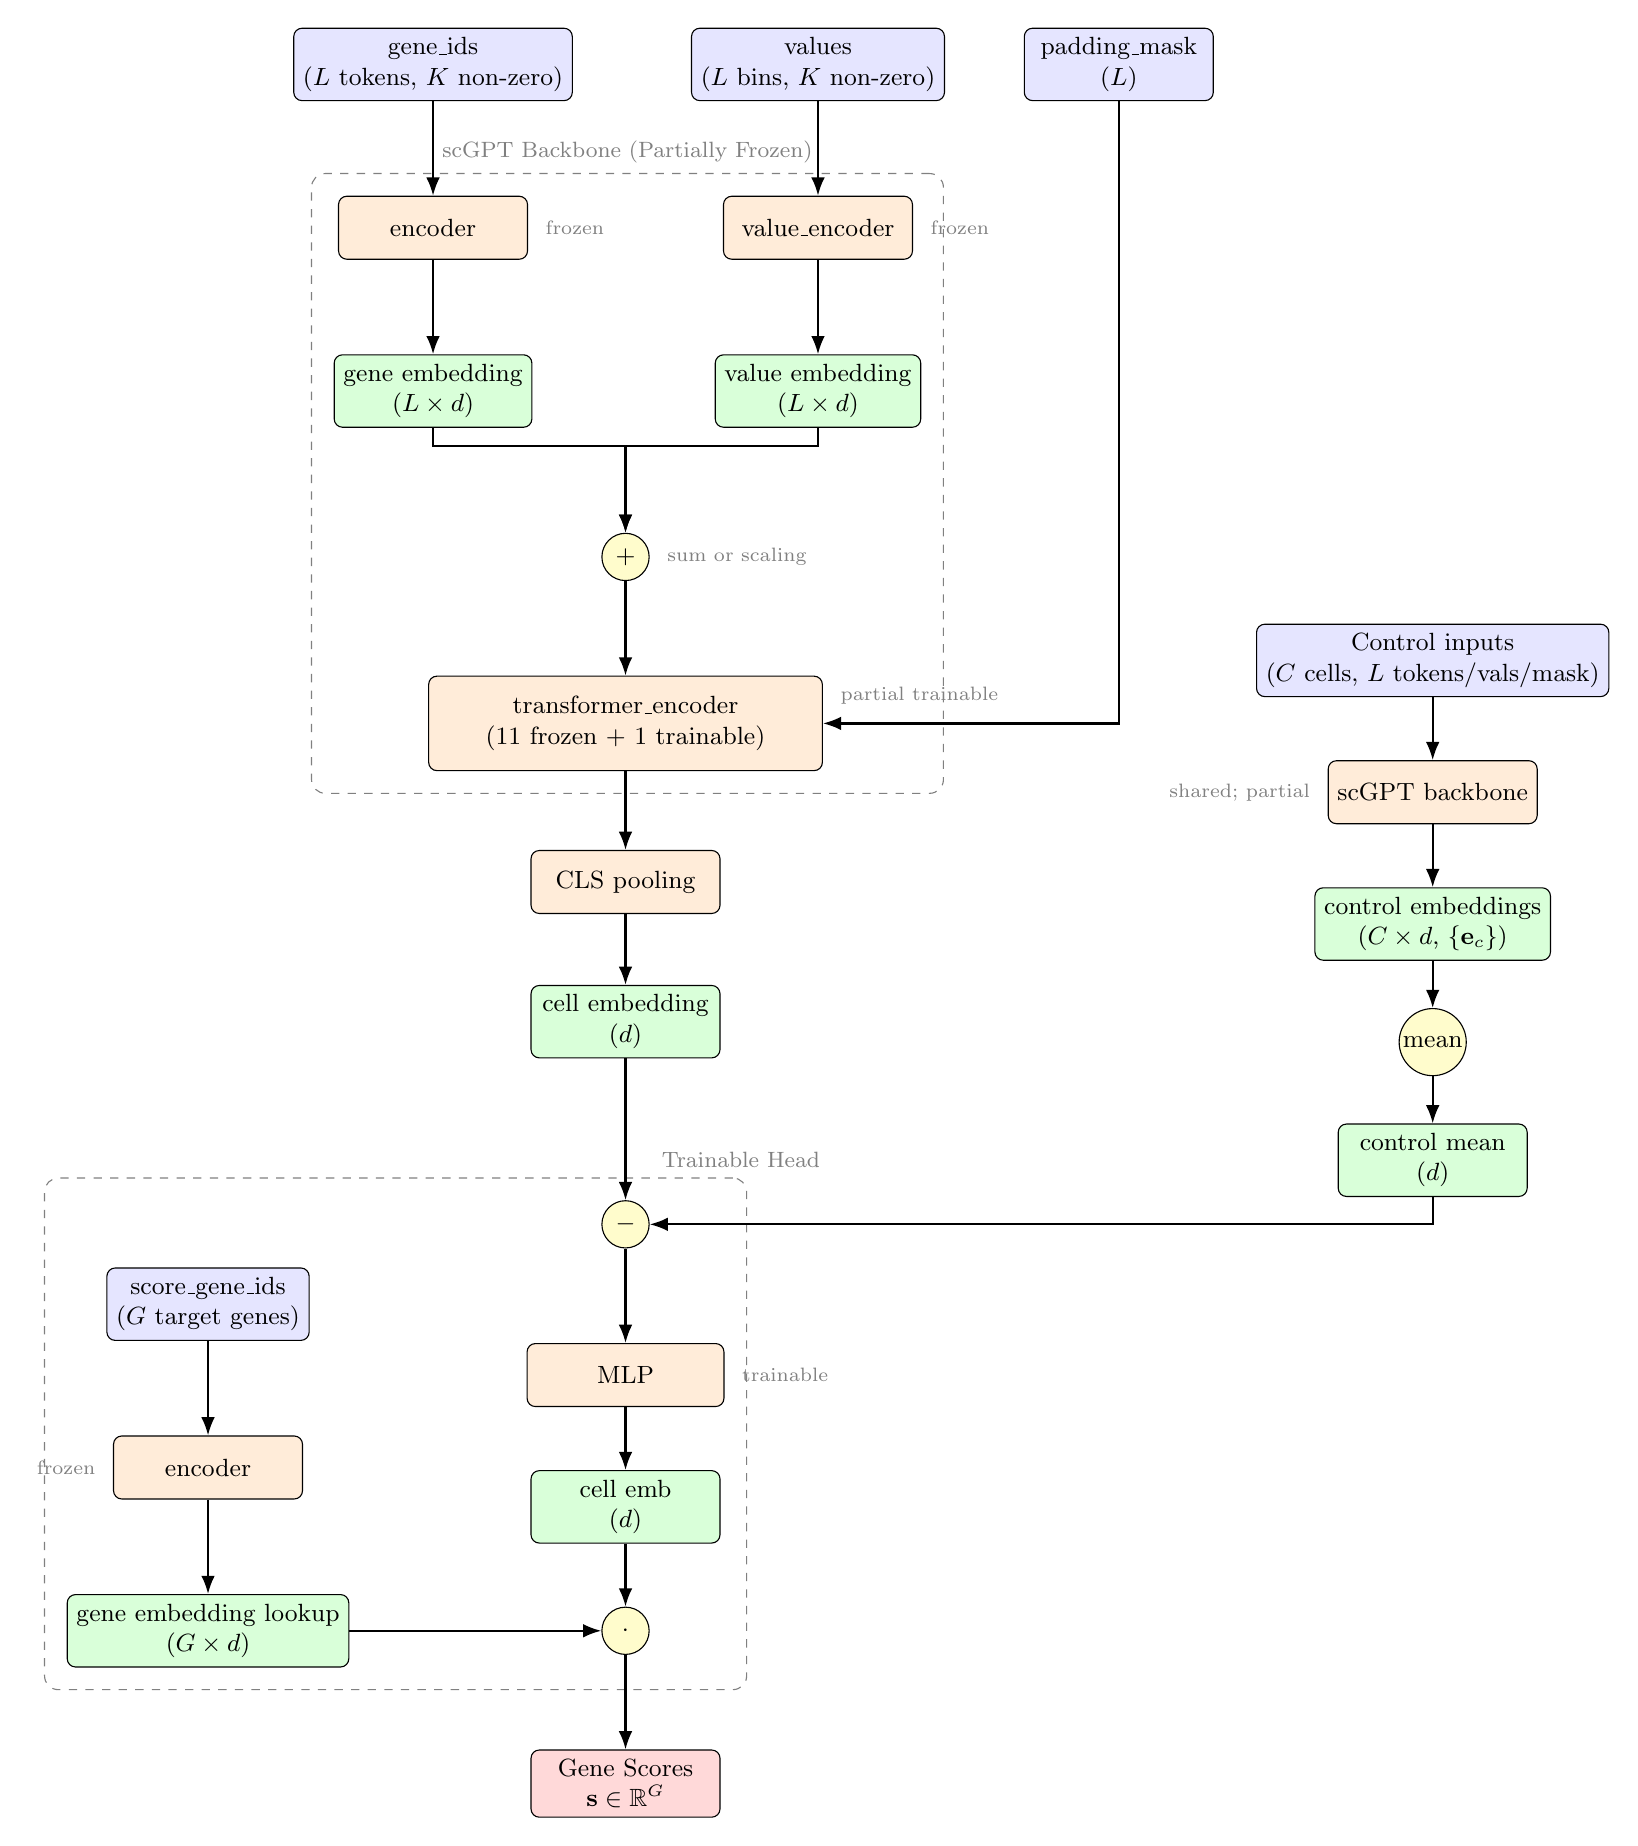
\begin{tikzpicture}[
    >=Latex,
    node distance=1.2cm and 2.4cm,
    font=\small,
    % Style definitions
    input/.style={draw, rounded corners=3pt, minimum width=2.4cm, minimum height=0.8cm, fill=blue!10, align=center},
    embed/.style={draw, rounded corners=3pt, minimum width=2.4cm, minimum height=0.8cm, fill=green!15, align=center},
    encoder/.style={draw, rounded corners=3pt, minimum width=2.4cm, minimum height=0.8cm, fill=orange!15, align=center},
    head/.style={draw, rounded corners=3pt, minimum width=2.4cm, minimum height=0.8cm, fill=yellow!15, align=center},
    unused/.style={draw, rounded corners=3pt, minimum width=2.4cm, minimum height=0.8cm, fill=gray!10, align=center, dashed},
    output/.style={draw, rounded corners=3pt, minimum width=2.4cm, minimum height=0.8cm, fill=red!15, align=center},
    operation/.style={circle, draw, minimum size=0.6cm, fill=yellow!20, inner sep=1pt},
    dashedbox/.style={draw, dashed, rounded corners=5pt, inner sep=8pt, gray},
    arrow/.style={->, thick, >=Latex, black},
]

%% ---------- INPUT LAYER ----------
\node[input] (gene_ids) {gene\_ids\\($L$ tokens, $K$ non-zero)};
\node[input, right=1.5cm of gene_ids] (values) {values\\($L$ bins, $K$ non-zero)};
\node[input, right=1cm of values] (padding) {padding\_mask\\($L$)};

%% ---------- ENCODERS + EMBEDDINGS (PARALLEL) ----------
\node[encoder, below=of gene_ids] (gene_encoder) {encoder};
\node[embed, below=of gene_encoder] (gene_emb) {gene embedding\\($L \times d$)};
\node[encoder, below=of values] (value_encoder) {value\_encoder};
\node[embed, below=of value_encoder] (value_emb) {value embedding\\($L \times d$)};

%% ---------- EMBEDDING FUSION ----------
\node[operation, below=1.8cm of $(gene_emb)!0.5!(value_emb)$] (add) {$+$};
\node[font=\scriptsize, gray, right=0.1cm of add.east] {sum or scaling};

%% ---------- TRANSFORMER ----------
\node[encoder, below=of add, minimum width=5cm, minimum height=1.2cm] (transformer) {transformer\_encoder\\(11 frozen + 1 trainable)};

%% ---------- OUTPUTS FROM TRANSFORMER ----------
\node[encoder, below=1.0cm of transformer] (cls_pool) {CLS pooling};
\node[embed, below=0.9cm of cls_pool] (cell_emb) {cell embedding\\($d$)};

%% ---------- CONTROL BRANCH ----------
\node[input, right=5.5cm of transformer, yshift=0.8cm] (control_branch) {Control inputs\\($C$ cells, $L$ tokens/vals/mask)};
\node[encoder, below=0.8cm of control_branch] (control_encoder) {scGPT backbone};
\node[embed, below=0.8cm of control_encoder] (control_emb) {control embeddings\\($C \times d$, $\{\mathbf{e}_c\}$)};
\node[operation, below=0.6cm of control_emb] (control_mean_op) {mean};
\node[embed, below=0.6cm of control_mean_op] (control_mean) {control mean\\($d$)};

%% ---------- DELTA EMBEDDING ----------
\node[operation, below=1.8cm of cell_emb] (subtract) {$-$};

%% ---------- GENE SCORING HEAD ----------
\node[encoder, below=of subtract, minimum width=2.5cm] (proj_mlp) {MLP};
\node[embed, below=0.8cm of proj_mlp] (cell_proj) {cell emb\\($d$)};
\node[operation, below=0.8cm of cell_proj] (dot_op) {$\cdot$};

%% ---------- OUTPUT ----------
\node[output, below=of dot_op] (scores) {Gene Scores\\$\mathbf{s} \in \mathbb{R}^{G}$};

%% ========== ARROWS ==========

% Inputs to encoders/embeddings
\draw[arrow] (gene_ids) -- (gene_encoder);
\draw[arrow] (gene_encoder) -- (gene_emb);
\draw[arrow] (values) -- (value_encoder);
\draw[arrow] (value_encoder) -- (value_emb);

% Embeddings to fusion (parallel)
\draw[arrow] (gene_emb) -- ++(0,-0.7) -| (add);
\draw[arrow] (value_emb) -- ++(0,-0.7) -| (add);

% Fusion to transformer
\draw[arrow] (add) -- (transformer);
\draw[arrow] (padding) |- (transformer);

% Transformer to cell embedding
\draw[arrow] (transformer.south) -- (cls_pool.north);
\draw[arrow] (cls_pool.south) -- (cell_emb.north);

% Control branch
\draw[arrow] (control_branch) -- (control_encoder);
\draw[arrow] (control_encoder) -- (control_emb);
\draw[arrow] (control_emb) -- (control_mean_op);
\draw[arrow] (control_mean_op) -- (control_mean);
\draw[arrow] (control_mean.south) |- (subtract.east);

% Cell embedding to delta
\draw[arrow] (cell_emb) -- (subtract);

% Delta to projection MLP
\draw[arrow] (subtract) -- (proj_mlp);
\draw[arrow] (proj_mlp) -- (cell_proj);
\draw[arrow] (cell_proj) -- (dot_op);

% Dot product to output
\draw[arrow] (dot_op) -- (scores);

% Gene embeddings to dot product (parallel flow)
\node[embed, left=3.2cm of dot_op] (gene_emb_lookup) {gene embedding lookup\\($G \times d$)};
\node[encoder, above=of gene_emb_lookup] (gene_emb_lookup_enc) {encoder};
\node[input, above=of gene_emb_lookup_enc] (score_gene_ids) {score\_gene\_ids\\($G$ target genes)};
\draw[arrow] (score_gene_ids) -- (gene_emb_lookup_enc);
\draw[arrow] (gene_emb_lookup_enc) -- (gene_emb_lookup);
\draw[arrow] (gene_emb_lookup.east) -- (dot_op.west);

%% ========== DASHED BOXES FOR GROUPING ==========

% scGPT Backbone box
\begin{scope}[on background layer]
    \node[dashedbox, fit=(gene_encoder)(value_encoder)(gene_emb)(value_emb)(add)(transformer), label={[font=\footnotesize, gray]above:scGPT Backbone (Partially Frozen)}] {};
\end{scope}

% Discriminative Head box
\begin{scope}[on background layer]
    \node[dashedbox, fit=(subtract)(proj_mlp)(cell_proj)(dot_op)(score_gene_ids)(gene_emb_lookup_enc)(gene_emb_lookup), label={[font=\footnotesize, gray]above right:Trainable Head}] {};
\end{scope}

%% ========== ANNOTATIONS ==========

% Trainability annotations
\node[font=\scriptsize, gray, right=0.1cm of gene_encoder.east] {frozen};
\node[font=\scriptsize, gray, right=0.1cm of value_encoder.east] {frozen};
\node[font=\scriptsize, gray, right=0.1cm of transformer.east, yshift=0.35cm] {partial trainable};
\node[font=\scriptsize, gray, left=0.1cm of control_encoder.west] {shared; partial};
\node[font=\scriptsize, gray, right=0.1cm of proj_mlp.east] {trainable};
\node[font=\scriptsize, gray, left=0.1cm of gene_emb_lookup_enc.west] {frozen};

\end{tikzpicture}
\ifexportfig
\else
\caption{Per-cell scGPT Discriminative Pipeline for Perturbation Gene Prediction.
For a single cell with $K$ non-zero genes, inputs are padded to length $L$.
Token IDs (\texttt{gene\_ids}), binned expression values, and a padding mask are fed to the scGPT backbone.
The \texttt{encoder} and \texttt{value\_encoder} produce gene/value embeddings, which are fused by element-wise addition (default)
or scaling (\texttt{input\_emb\_style}=\texttt{scaling}), then passed through \texttt{transformer\_encoder} to produce a CLS-based cell embedding.
A control branch runs the same backbone and the control mean is subtracted from the perturbed embedding.
The GeneScore head applies a projection MLP to the cell embedding before the dot product with the gene embedding lookup.
The \texttt{score\_gene\_ids} input is length $G$, the full set of candidate target genes, and its order defines the score output columns.
The backbone is partially frozen in this setup, with only the last transformer layer(s) and encoder norm optionally trainable.
Here, $G$ is the total number of genes in the dataset, $C$ is the number of control cells per perturbed cell, and $d$ is the embedding size.}
\label{fig:scgpt_pipeline}
\fi
\end{figure}

\end{document}
"
%   latex -interaction=nonstopmode -halt-on-error -jobname scGPT_pipeline_standalone_export -output-directory docs/report/final_report "\\def\\EXPORTFIG{1}\% scGPT Discriminative Pipeline Architecture (Standalone)
% Export (caption-free) SVG/PNG:
%   pdflatex -interaction=nonstopmode -halt-on-error -jobname scGPT_pipeline_standalone_export -output-directory docs/report/final_report "\\def\\EXPORTFIG{1}\\input{docs/report/final_report/scGPT_pipeline_standalone.tex}"
%   latex -interaction=nonstopmode -halt-on-error -jobname scGPT_pipeline_standalone_export -output-directory docs/report/final_report "\\def\\EXPORTFIG{1}\\input{docs/report/final_report/scGPT_pipeline_standalone.tex}"
%   dvisvgm --libgs=/opt/homebrew/lib/libgs.dylib -o docs/report/final_report/scGPT_pipeline_standalone.svg docs/report/final_report/scGPT_pipeline_standalone_export.dvi
%   gs -sDEVICE=pngalpha -r300 -o docs/report/final_report/scGPT_pipeline_standalone.png docs/report/final_report/scGPT_pipeline_standalone_export.pdf

\documentclass{article}
\usepackage[margin=1cm]{geometry}
\usepackage{tikz}
\usepackage{amsmath,amssymb}
\usetikzlibrary{arrows.meta, positioning, shapes.geometric, calc, fit, backgrounds}
\newif\ifexportfig
\ifdefined\EXPORTFIG
\exportfigtrue
\else
\exportfigfalse
\fi

\begin{document}
\pagecolor{white}

\begin{figure}[htbp]
\centering
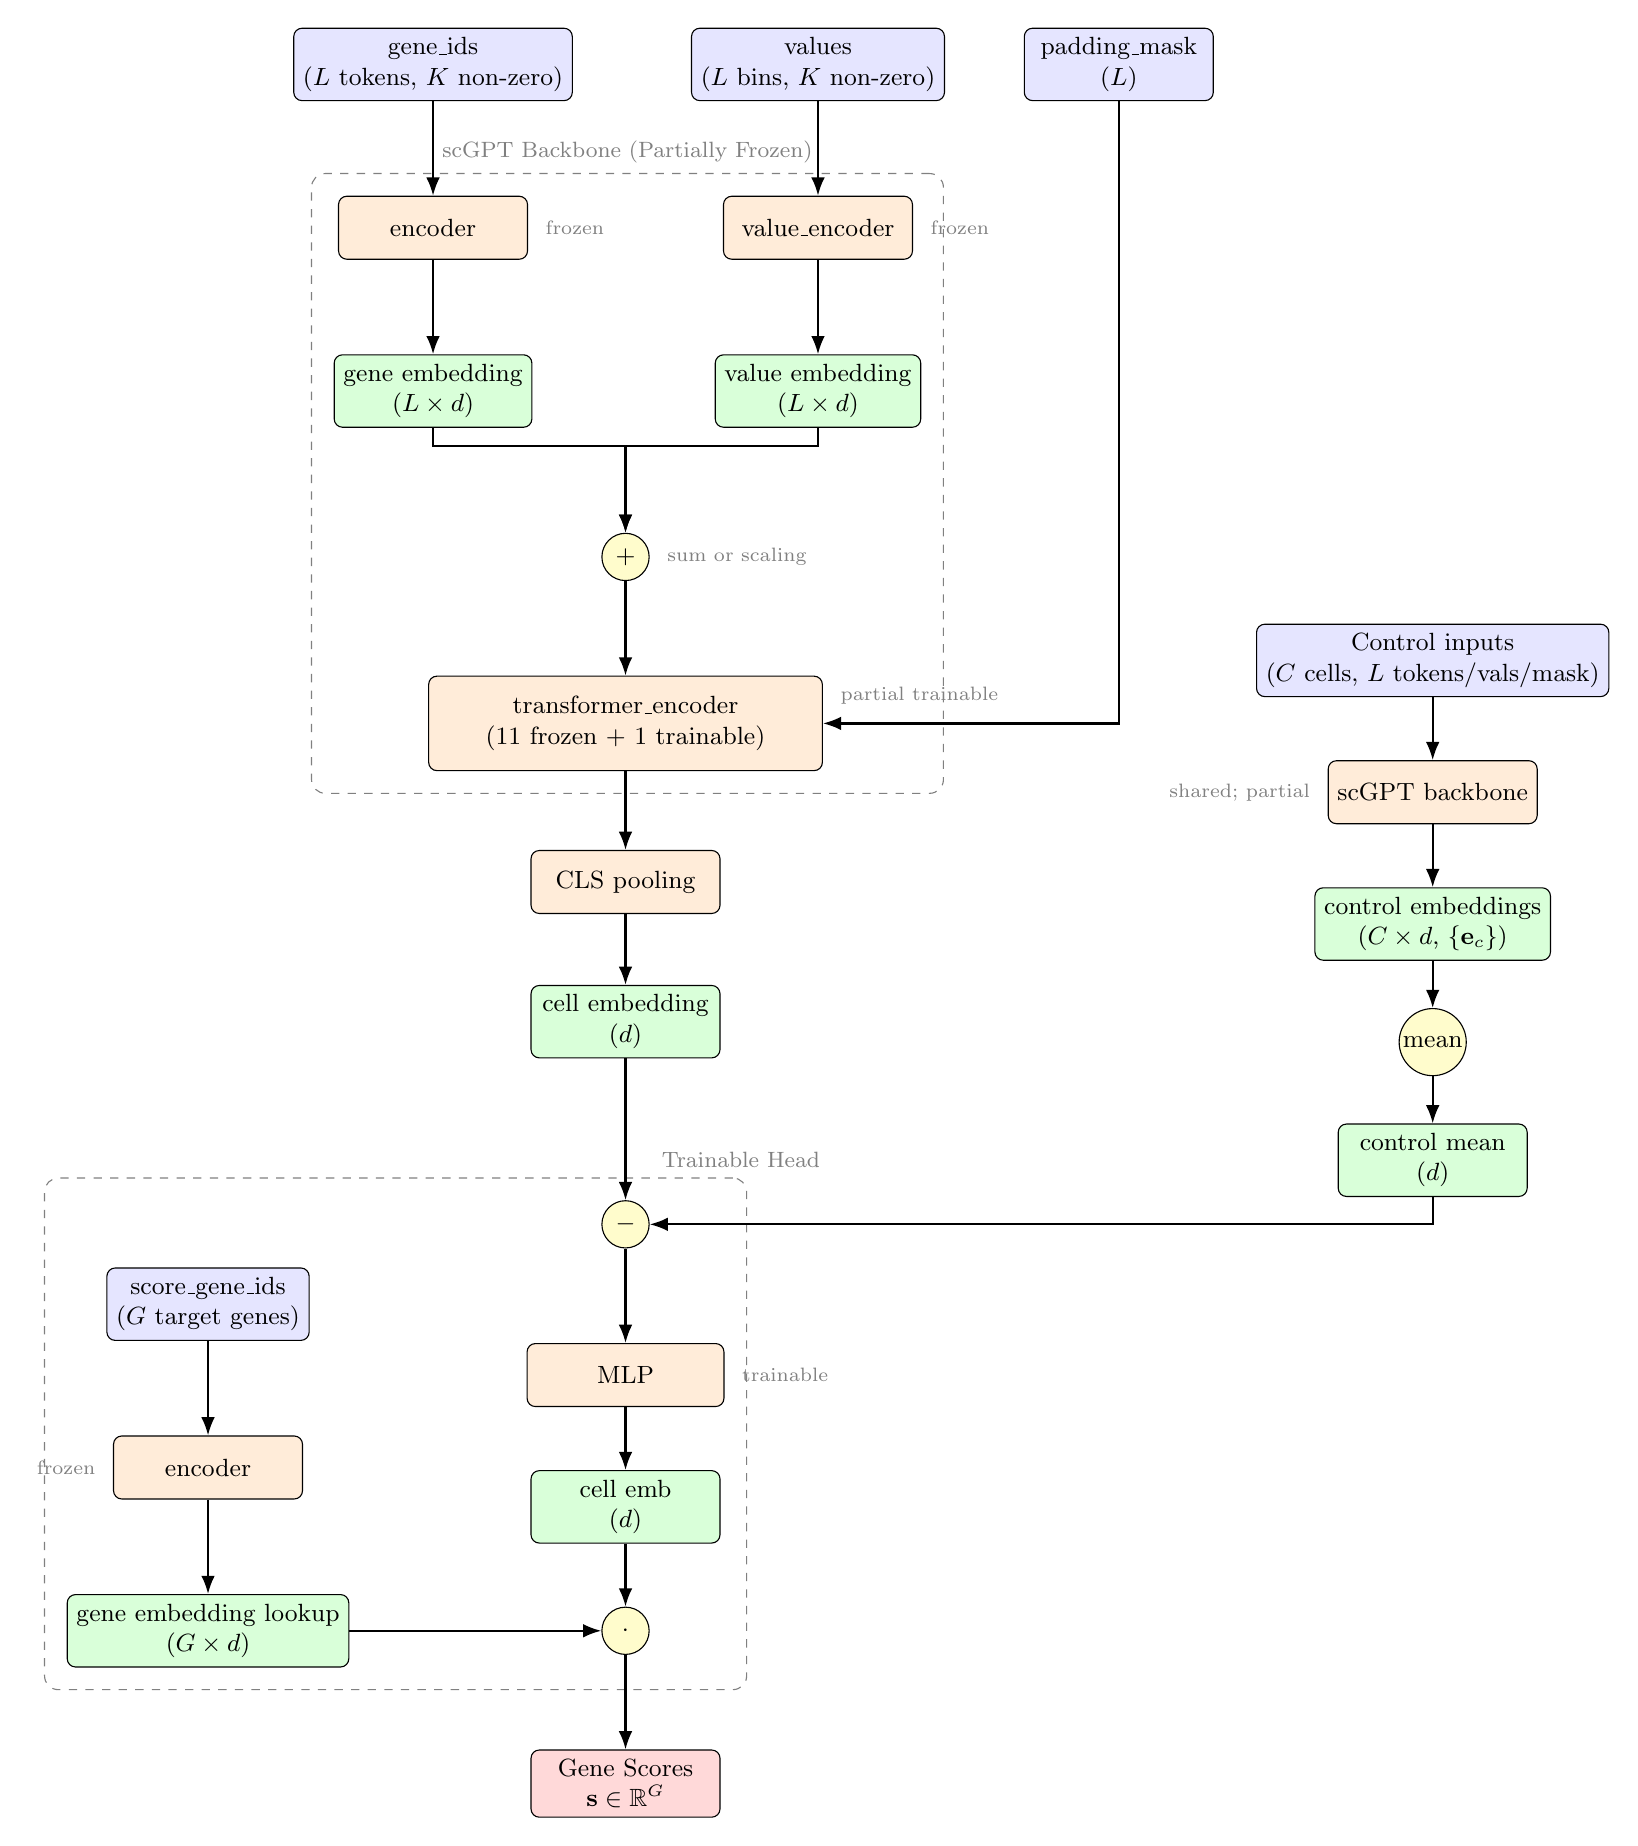
\begin{tikzpicture}[
    >=Latex,
    node distance=1.2cm and 2.4cm,
    font=\small,
    % Style definitions
    input/.style={draw, rounded corners=3pt, minimum width=2.4cm, minimum height=0.8cm, fill=blue!10, align=center},
    embed/.style={draw, rounded corners=3pt, minimum width=2.4cm, minimum height=0.8cm, fill=green!15, align=center},
    encoder/.style={draw, rounded corners=3pt, minimum width=2.4cm, minimum height=0.8cm, fill=orange!15, align=center},
    head/.style={draw, rounded corners=3pt, minimum width=2.4cm, minimum height=0.8cm, fill=yellow!15, align=center},
    unused/.style={draw, rounded corners=3pt, minimum width=2.4cm, minimum height=0.8cm, fill=gray!10, align=center, dashed},
    output/.style={draw, rounded corners=3pt, minimum width=2.4cm, minimum height=0.8cm, fill=red!15, align=center},
    operation/.style={circle, draw, minimum size=0.6cm, fill=yellow!20, inner sep=1pt},
    dashedbox/.style={draw, dashed, rounded corners=5pt, inner sep=8pt, gray},
    arrow/.style={->, thick, >=Latex, black},
]

%% ---------- INPUT LAYER ----------
\node[input] (gene_ids) {gene\_ids\\($L$ tokens, $K$ non-zero)};
\node[input, right=1.5cm of gene_ids] (values) {values\\($L$ bins, $K$ non-zero)};
\node[input, right=1cm of values] (padding) {padding\_mask\\($L$)};

%% ---------- ENCODERS + EMBEDDINGS (PARALLEL) ----------
\node[encoder, below=of gene_ids] (gene_encoder) {encoder};
\node[embed, below=of gene_encoder] (gene_emb) {gene embedding\\($L \times d$)};
\node[encoder, below=of values] (value_encoder) {value\_encoder};
\node[embed, below=of value_encoder] (value_emb) {value embedding\\($L \times d$)};

%% ---------- EMBEDDING FUSION ----------
\node[operation, below=1.8cm of $(gene_emb)!0.5!(value_emb)$] (add) {$+$};
\node[font=\scriptsize, gray, right=0.1cm of add.east] {sum or scaling};

%% ---------- TRANSFORMER ----------
\node[encoder, below=of add, minimum width=5cm, minimum height=1.2cm] (transformer) {transformer\_encoder\\(11 frozen + 1 trainable)};

%% ---------- OUTPUTS FROM TRANSFORMER ----------
\node[encoder, below=1.0cm of transformer] (cls_pool) {CLS pooling};
\node[embed, below=0.9cm of cls_pool] (cell_emb) {cell embedding\\($d$)};

%% ---------- CONTROL BRANCH ----------
\node[input, right=5.5cm of transformer, yshift=0.8cm] (control_branch) {Control inputs\\($C$ cells, $L$ tokens/vals/mask)};
\node[encoder, below=0.8cm of control_branch] (control_encoder) {scGPT backbone};
\node[embed, below=0.8cm of control_encoder] (control_emb) {control embeddings\\($C \times d$, $\{\mathbf{e}_c\}$)};
\node[operation, below=0.6cm of control_emb] (control_mean_op) {mean};
\node[embed, below=0.6cm of control_mean_op] (control_mean) {control mean\\($d$)};

%% ---------- DELTA EMBEDDING ----------
\node[operation, below=1.8cm of cell_emb] (subtract) {$-$};

%% ---------- GENE SCORING HEAD ----------
\node[encoder, below=of subtract, minimum width=2.5cm] (proj_mlp) {MLP};
\node[embed, below=0.8cm of proj_mlp] (cell_proj) {cell emb\\($d$)};
\node[operation, below=0.8cm of cell_proj] (dot_op) {$\cdot$};

%% ---------- OUTPUT ----------
\node[output, below=of dot_op] (scores) {Gene Scores\\$\mathbf{s} \in \mathbb{R}^{G}$};

%% ========== ARROWS ==========

% Inputs to encoders/embeddings
\draw[arrow] (gene_ids) -- (gene_encoder);
\draw[arrow] (gene_encoder) -- (gene_emb);
\draw[arrow] (values) -- (value_encoder);
\draw[arrow] (value_encoder) -- (value_emb);

% Embeddings to fusion (parallel)
\draw[arrow] (gene_emb) -- ++(0,-0.7) -| (add);
\draw[arrow] (value_emb) -- ++(0,-0.7) -| (add);

% Fusion to transformer
\draw[arrow] (add) -- (transformer);
\draw[arrow] (padding) |- (transformer);

% Transformer to cell embedding
\draw[arrow] (transformer.south) -- (cls_pool.north);
\draw[arrow] (cls_pool.south) -- (cell_emb.north);

% Control branch
\draw[arrow] (control_branch) -- (control_encoder);
\draw[arrow] (control_encoder) -- (control_emb);
\draw[arrow] (control_emb) -- (control_mean_op);
\draw[arrow] (control_mean_op) -- (control_mean);
\draw[arrow] (control_mean.south) |- (subtract.east);

% Cell embedding to delta
\draw[arrow] (cell_emb) -- (subtract);

% Delta to projection MLP
\draw[arrow] (subtract) -- (proj_mlp);
\draw[arrow] (proj_mlp) -- (cell_proj);
\draw[arrow] (cell_proj) -- (dot_op);

% Dot product to output
\draw[arrow] (dot_op) -- (scores);

% Gene embeddings to dot product (parallel flow)
\node[embed, left=3.2cm of dot_op] (gene_emb_lookup) {gene embedding lookup\\($G \times d$)};
\node[encoder, above=of gene_emb_lookup] (gene_emb_lookup_enc) {encoder};
\node[input, above=of gene_emb_lookup_enc] (score_gene_ids) {score\_gene\_ids\\($G$ target genes)};
\draw[arrow] (score_gene_ids) -- (gene_emb_lookup_enc);
\draw[arrow] (gene_emb_lookup_enc) -- (gene_emb_lookup);
\draw[arrow] (gene_emb_lookup.east) -- (dot_op.west);

%% ========== DASHED BOXES FOR GROUPING ==========

% scGPT Backbone box
\begin{scope}[on background layer]
    \node[dashedbox, fit=(gene_encoder)(value_encoder)(gene_emb)(value_emb)(add)(transformer), label={[font=\footnotesize, gray]above:scGPT Backbone (Partially Frozen)}] {};
\end{scope}

% Discriminative Head box
\begin{scope}[on background layer]
    \node[dashedbox, fit=(subtract)(proj_mlp)(cell_proj)(dot_op)(score_gene_ids)(gene_emb_lookup_enc)(gene_emb_lookup), label={[font=\footnotesize, gray]above right:Trainable Head}] {};
\end{scope}

%% ========== ANNOTATIONS ==========

% Trainability annotations
\node[font=\scriptsize, gray, right=0.1cm of gene_encoder.east] {frozen};
\node[font=\scriptsize, gray, right=0.1cm of value_encoder.east] {frozen};
\node[font=\scriptsize, gray, right=0.1cm of transformer.east, yshift=0.35cm] {partial trainable};
\node[font=\scriptsize, gray, left=0.1cm of control_encoder.west] {shared; partial};
\node[font=\scriptsize, gray, right=0.1cm of proj_mlp.east] {trainable};
\node[font=\scriptsize, gray, left=0.1cm of gene_emb_lookup_enc.west] {frozen};

\end{tikzpicture}
\ifexportfig
\else
\caption{Per-cell scGPT Discriminative Pipeline for Perturbation Gene Prediction.
For a single cell with $K$ non-zero genes, inputs are padded to length $L$.
Token IDs (\texttt{gene\_ids}), binned expression values, and a padding mask are fed to the scGPT backbone.
The \texttt{encoder} and \texttt{value\_encoder} produce gene/value embeddings, which are fused by element-wise addition (default)
or scaling (\texttt{input\_emb\_style}=\texttt{scaling}), then passed through \texttt{transformer\_encoder} to produce a CLS-based cell embedding.
A control branch runs the same backbone and the control mean is subtracted from the perturbed embedding.
The GeneScore head applies a projection MLP to the cell embedding before the dot product with the gene embedding lookup.
The \texttt{score\_gene\_ids} input is length $G$, the full set of candidate target genes, and its order defines the score output columns.
The backbone is partially frozen in this setup, with only the last transformer layer(s) and encoder norm optionally trainable.
Here, $G$ is the total number of genes in the dataset, $C$ is the number of control cells per perturbed cell, and $d$ is the embedding size.}
\label{fig:scgpt_pipeline}
\fi
\end{figure}

\end{document}
"
%   dvisvgm --libgs=/opt/homebrew/lib/libgs.dylib -o docs/report/final_report/scGPT_pipeline_standalone.svg docs/report/final_report/scGPT_pipeline_standalone_export.dvi
%   gs -sDEVICE=pngalpha -r300 -o docs/report/final_report/scGPT_pipeline_standalone.png docs/report/final_report/scGPT_pipeline_standalone_export.pdf

\documentclass{article}
\usepackage[margin=1cm]{geometry}
\usepackage{tikz}
\usepackage{amsmath,amssymb}
\usetikzlibrary{arrows.meta, positioning, shapes.geometric, calc, fit, backgrounds}
\newif\ifexportfig
\ifdefined\EXPORTFIG
\exportfigtrue
\else
\exportfigfalse
\fi

\begin{document}
\pagecolor{white}

\begin{figure}[htbp]
\centering
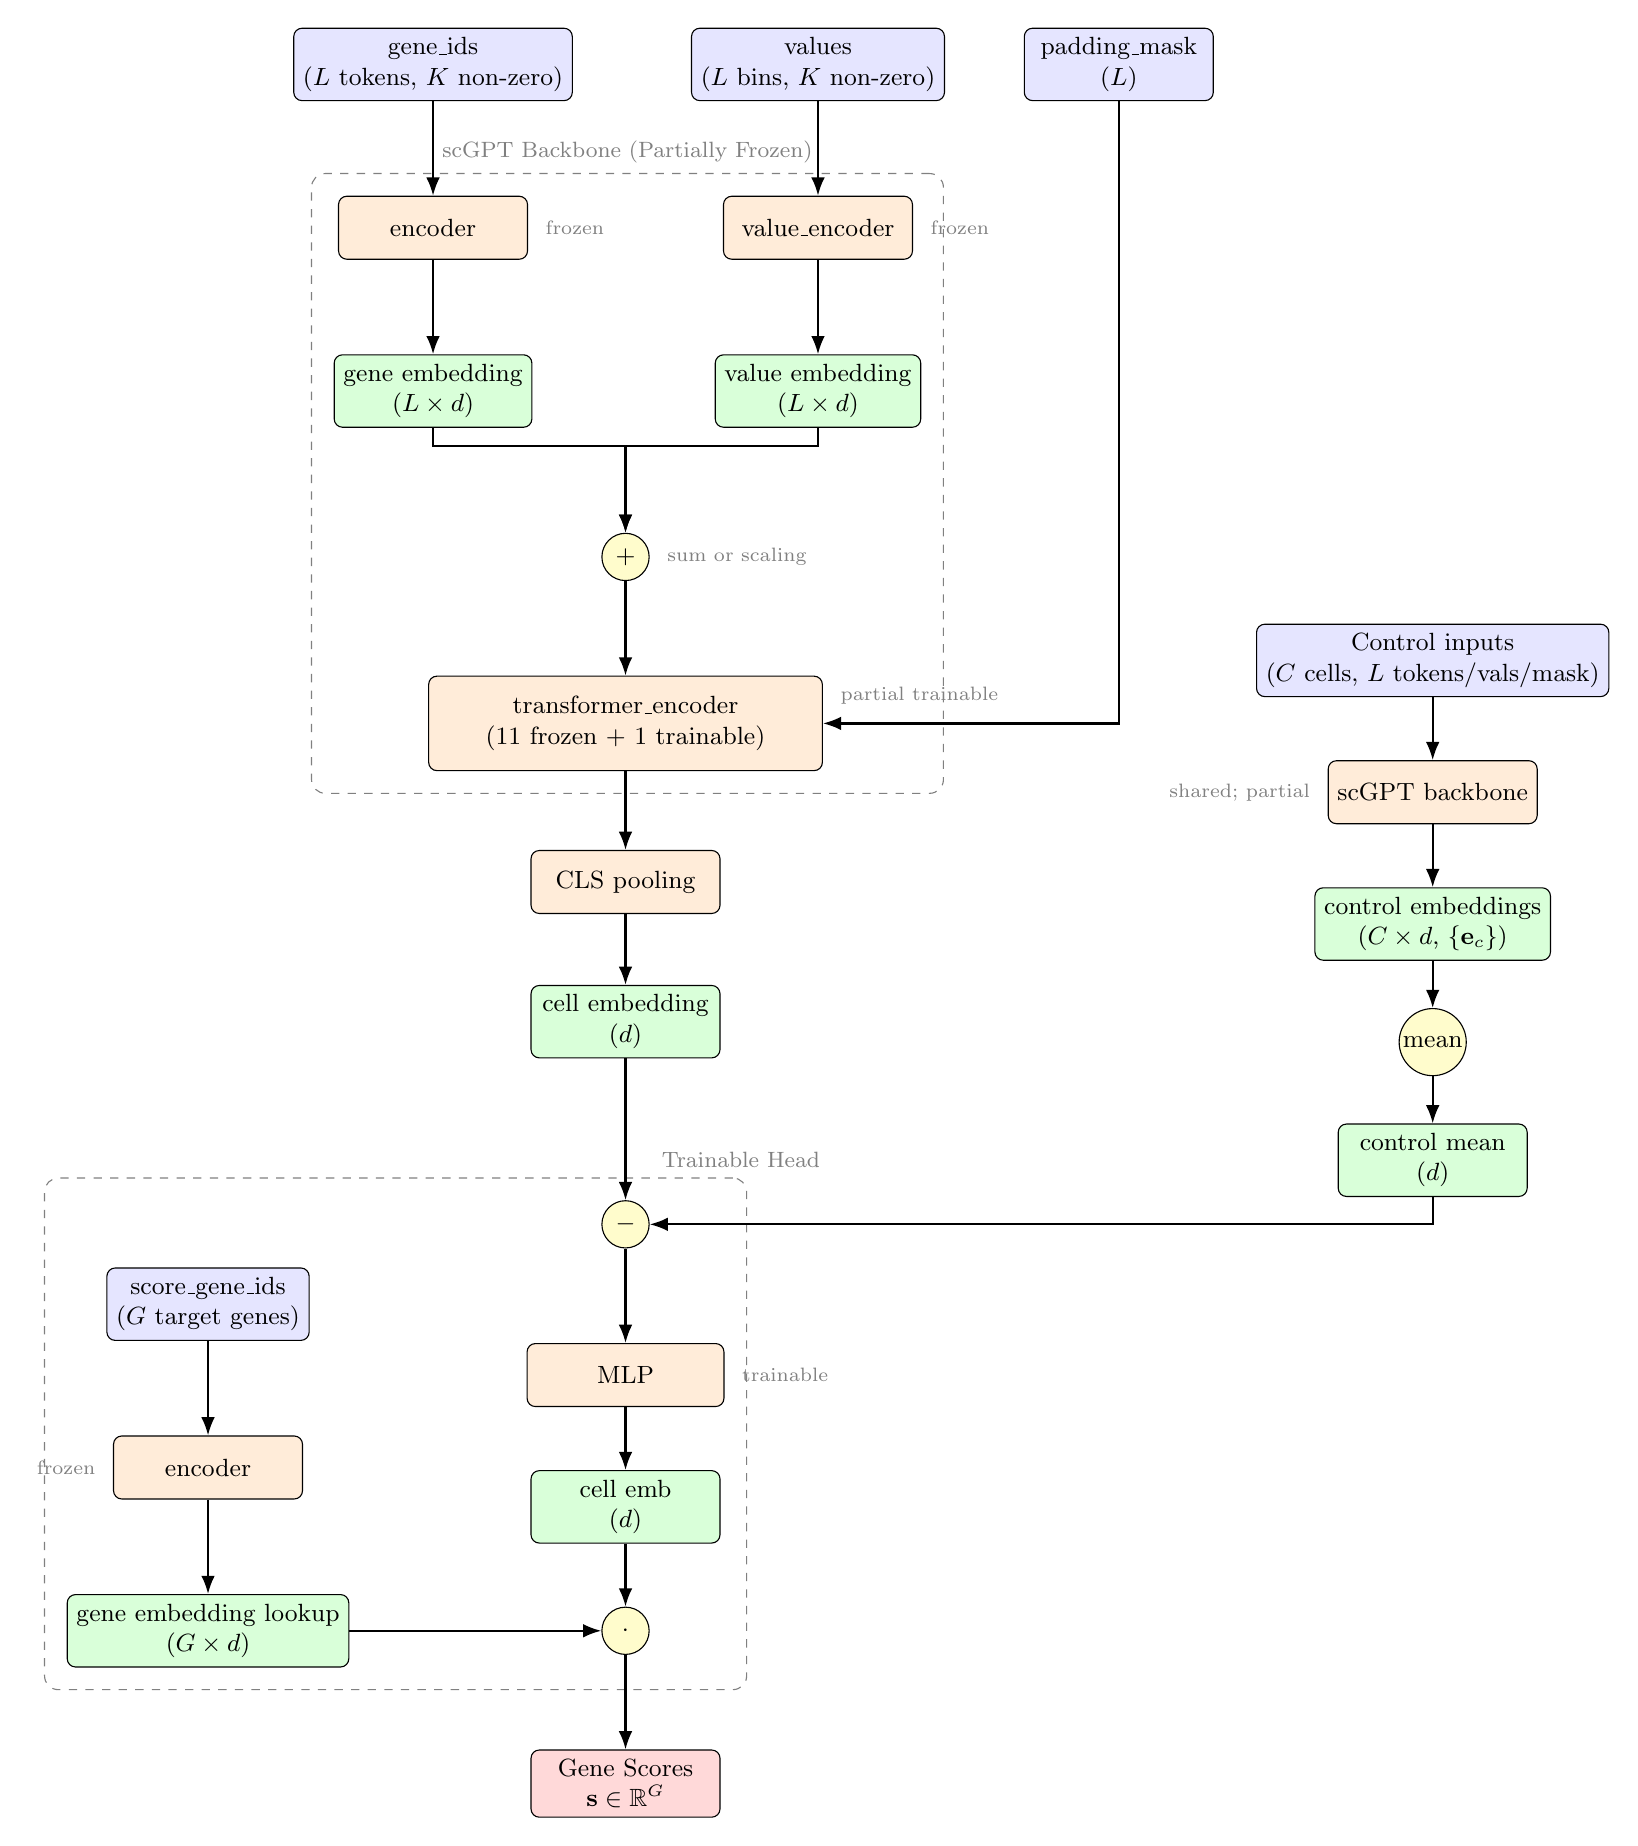
\begin{tikzpicture}[
    >=Latex,
    node distance=1.2cm and 2.4cm,
    font=\small,
    % Style definitions
    input/.style={draw, rounded corners=3pt, minimum width=2.4cm, minimum height=0.8cm, fill=blue!10, align=center},
    embed/.style={draw, rounded corners=3pt, minimum width=2.4cm, minimum height=0.8cm, fill=green!15, align=center},
    encoder/.style={draw, rounded corners=3pt, minimum width=2.4cm, minimum height=0.8cm, fill=orange!15, align=center},
    head/.style={draw, rounded corners=3pt, minimum width=2.4cm, minimum height=0.8cm, fill=yellow!15, align=center},
    unused/.style={draw, rounded corners=3pt, minimum width=2.4cm, minimum height=0.8cm, fill=gray!10, align=center, dashed},
    output/.style={draw, rounded corners=3pt, minimum width=2.4cm, minimum height=0.8cm, fill=red!15, align=center},
    operation/.style={circle, draw, minimum size=0.6cm, fill=yellow!20, inner sep=1pt},
    dashedbox/.style={draw, dashed, rounded corners=5pt, inner sep=8pt, gray},
    arrow/.style={->, thick, >=Latex, black},
]

%% ---------- INPUT LAYER ----------
\node[input] (gene_ids) {gene\_ids\\($L$ tokens, $K$ non-zero)};
\node[input, right=1.5cm of gene_ids] (values) {values\\($L$ bins, $K$ non-zero)};
\node[input, right=1cm of values] (padding) {padding\_mask\\($L$)};

%% ---------- ENCODERS + EMBEDDINGS (PARALLEL) ----------
\node[encoder, below=of gene_ids] (gene_encoder) {encoder};
\node[embed, below=of gene_encoder] (gene_emb) {gene embedding\\($L \times d$)};
\node[encoder, below=of values] (value_encoder) {value\_encoder};
\node[embed, below=of value_encoder] (value_emb) {value embedding\\($L \times d$)};

%% ---------- EMBEDDING FUSION ----------
\node[operation, below=1.8cm of $(gene_emb)!0.5!(value_emb)$] (add) {$+$};
\node[font=\scriptsize, gray, right=0.1cm of add.east] {sum or scaling};

%% ---------- TRANSFORMER ----------
\node[encoder, below=of add, minimum width=5cm, minimum height=1.2cm] (transformer) {transformer\_encoder\\(11 frozen + 1 trainable)};

%% ---------- OUTPUTS FROM TRANSFORMER ----------
\node[encoder, below=1.0cm of transformer] (cls_pool) {CLS pooling};
\node[embed, below=0.9cm of cls_pool] (cell_emb) {cell embedding\\($d$)};

%% ---------- CONTROL BRANCH ----------
\node[input, right=5.5cm of transformer, yshift=0.8cm] (control_branch) {Control inputs\\($C$ cells, $L$ tokens/vals/mask)};
\node[encoder, below=0.8cm of control_branch] (control_encoder) {scGPT backbone};
\node[embed, below=0.8cm of control_encoder] (control_emb) {control embeddings\\($C \times d$, $\{\mathbf{e}_c\}$)};
\node[operation, below=0.6cm of control_emb] (control_mean_op) {mean};
\node[embed, below=0.6cm of control_mean_op] (control_mean) {control mean\\($d$)};

%% ---------- DELTA EMBEDDING ----------
\node[operation, below=1.8cm of cell_emb] (subtract) {$-$};

%% ---------- GENE SCORING HEAD ----------
\node[encoder, below=of subtract, minimum width=2.5cm] (proj_mlp) {MLP};
\node[embed, below=0.8cm of proj_mlp] (cell_proj) {cell emb\\($d$)};
\node[operation, below=0.8cm of cell_proj] (dot_op) {$\cdot$};

%% ---------- OUTPUT ----------
\node[output, below=of dot_op] (scores) {Gene Scores\\$\mathbf{s} \in \mathbb{R}^{G}$};

%% ========== ARROWS ==========

% Inputs to encoders/embeddings
\draw[arrow] (gene_ids) -- (gene_encoder);
\draw[arrow] (gene_encoder) -- (gene_emb);
\draw[arrow] (values) -- (value_encoder);
\draw[arrow] (value_encoder) -- (value_emb);

% Embeddings to fusion (parallel)
\draw[arrow] (gene_emb) -- ++(0,-0.7) -| (add);
\draw[arrow] (value_emb) -- ++(0,-0.7) -| (add);

% Fusion to transformer
\draw[arrow] (add) -- (transformer);
\draw[arrow] (padding) |- (transformer);

% Transformer to cell embedding
\draw[arrow] (transformer.south) -- (cls_pool.north);
\draw[arrow] (cls_pool.south) -- (cell_emb.north);

% Control branch
\draw[arrow] (control_branch) -- (control_encoder);
\draw[arrow] (control_encoder) -- (control_emb);
\draw[arrow] (control_emb) -- (control_mean_op);
\draw[arrow] (control_mean_op) -- (control_mean);
\draw[arrow] (control_mean.south) |- (subtract.east);

% Cell embedding to delta
\draw[arrow] (cell_emb) -- (subtract);

% Delta to projection MLP
\draw[arrow] (subtract) -- (proj_mlp);
\draw[arrow] (proj_mlp) -- (cell_proj);
\draw[arrow] (cell_proj) -- (dot_op);

% Dot product to output
\draw[arrow] (dot_op) -- (scores);

% Gene embeddings to dot product (parallel flow)
\node[embed, left=3.2cm of dot_op] (gene_emb_lookup) {gene embedding lookup\\($G \times d$)};
\node[encoder, above=of gene_emb_lookup] (gene_emb_lookup_enc) {encoder};
\node[input, above=of gene_emb_lookup_enc] (score_gene_ids) {score\_gene\_ids\\($G$ target genes)};
\draw[arrow] (score_gene_ids) -- (gene_emb_lookup_enc);
\draw[arrow] (gene_emb_lookup_enc) -- (gene_emb_lookup);
\draw[arrow] (gene_emb_lookup.east) -- (dot_op.west);

%% ========== DASHED BOXES FOR GROUPING ==========

% scGPT Backbone box
\begin{scope}[on background layer]
    \node[dashedbox, fit=(gene_encoder)(value_encoder)(gene_emb)(value_emb)(add)(transformer), label={[font=\footnotesize, gray]above:scGPT Backbone (Partially Frozen)}] {};
\end{scope}

% Discriminative Head box
\begin{scope}[on background layer]
    \node[dashedbox, fit=(subtract)(proj_mlp)(cell_proj)(dot_op)(score_gene_ids)(gene_emb_lookup_enc)(gene_emb_lookup), label={[font=\footnotesize, gray]above right:Trainable Head}] {};
\end{scope}

%% ========== ANNOTATIONS ==========

% Trainability annotations
\node[font=\scriptsize, gray, right=0.1cm of gene_encoder.east] {frozen};
\node[font=\scriptsize, gray, right=0.1cm of value_encoder.east] {frozen};
\node[font=\scriptsize, gray, right=0.1cm of transformer.east, yshift=0.35cm] {partial trainable};
\node[font=\scriptsize, gray, left=0.1cm of control_encoder.west] {shared; partial};
\node[font=\scriptsize, gray, right=0.1cm of proj_mlp.east] {trainable};
\node[font=\scriptsize, gray, left=0.1cm of gene_emb_lookup_enc.west] {frozen};

\end{tikzpicture}
\ifexportfig
\else
\caption{Per-cell scGPT Discriminative Pipeline for Perturbation Gene Prediction.
For a single cell with $K$ non-zero genes, inputs are padded to length $L$.
Token IDs (\texttt{gene\_ids}), binned expression values, and a padding mask are fed to the scGPT backbone.
The \texttt{encoder} and \texttt{value\_encoder} produce gene/value embeddings, which are fused by element-wise addition (default)
or scaling (\texttt{input\_emb\_style}=\texttt{scaling}), then passed through \texttt{transformer\_encoder} to produce a CLS-based cell embedding.
A control branch runs the same backbone and the control mean is subtracted from the perturbed embedding.
The GeneScore head applies a projection MLP to the cell embedding before the dot product with the gene embedding lookup.
The \texttt{score\_gene\_ids} input is length $G$, the full set of candidate target genes, and its order defines the score output columns.
The backbone is partially frozen in this setup, with only the last transformer layer(s) and encoder norm optionally trainable.
Here, $G$ is the total number of genes in the dataset, $C$ is the number of control cells per perturbed cell, and $d$ is the embedding size.}
\label{fig:scgpt_pipeline}
\fi
\end{figure}

\end{document}
"
%   latex -interaction=nonstopmode -halt-on-error -jobname scGPT_pipeline_standalone_export -output-directory docs/report/final_report "\\def\\EXPORTFIG{1}\% scGPT Discriminative Pipeline Architecture (Standalone)
% Export (caption-free) SVG/PNG:
%   pdflatex -interaction=nonstopmode -halt-on-error -jobname scGPT_pipeline_standalone_export -output-directory docs/report/final_report "\\def\\EXPORTFIG{1}\% scGPT Discriminative Pipeline Architecture (Standalone)
% Export (caption-free) SVG/PNG:
%   pdflatex -interaction=nonstopmode -halt-on-error -jobname scGPT_pipeline_standalone_export -output-directory docs/report/final_report "\\def\\EXPORTFIG{1}\\input{docs/report/final_report/scGPT_pipeline_standalone.tex}"
%   latex -interaction=nonstopmode -halt-on-error -jobname scGPT_pipeline_standalone_export -output-directory docs/report/final_report "\\def\\EXPORTFIG{1}\\input{docs/report/final_report/scGPT_pipeline_standalone.tex}"
%   dvisvgm --libgs=/opt/homebrew/lib/libgs.dylib -o docs/report/final_report/scGPT_pipeline_standalone.svg docs/report/final_report/scGPT_pipeline_standalone_export.dvi
%   gs -sDEVICE=pngalpha -r300 -o docs/report/final_report/scGPT_pipeline_standalone.png docs/report/final_report/scGPT_pipeline_standalone_export.pdf

\documentclass{article}
\usepackage[margin=1cm]{geometry}
\usepackage{tikz}
\usepackage{amsmath,amssymb}
\usetikzlibrary{arrows.meta, positioning, shapes.geometric, calc, fit, backgrounds}
\newif\ifexportfig
\ifdefined\EXPORTFIG
\exportfigtrue
\else
\exportfigfalse
\fi

\begin{document}
\pagecolor{white}

\begin{figure}[htbp]
\centering
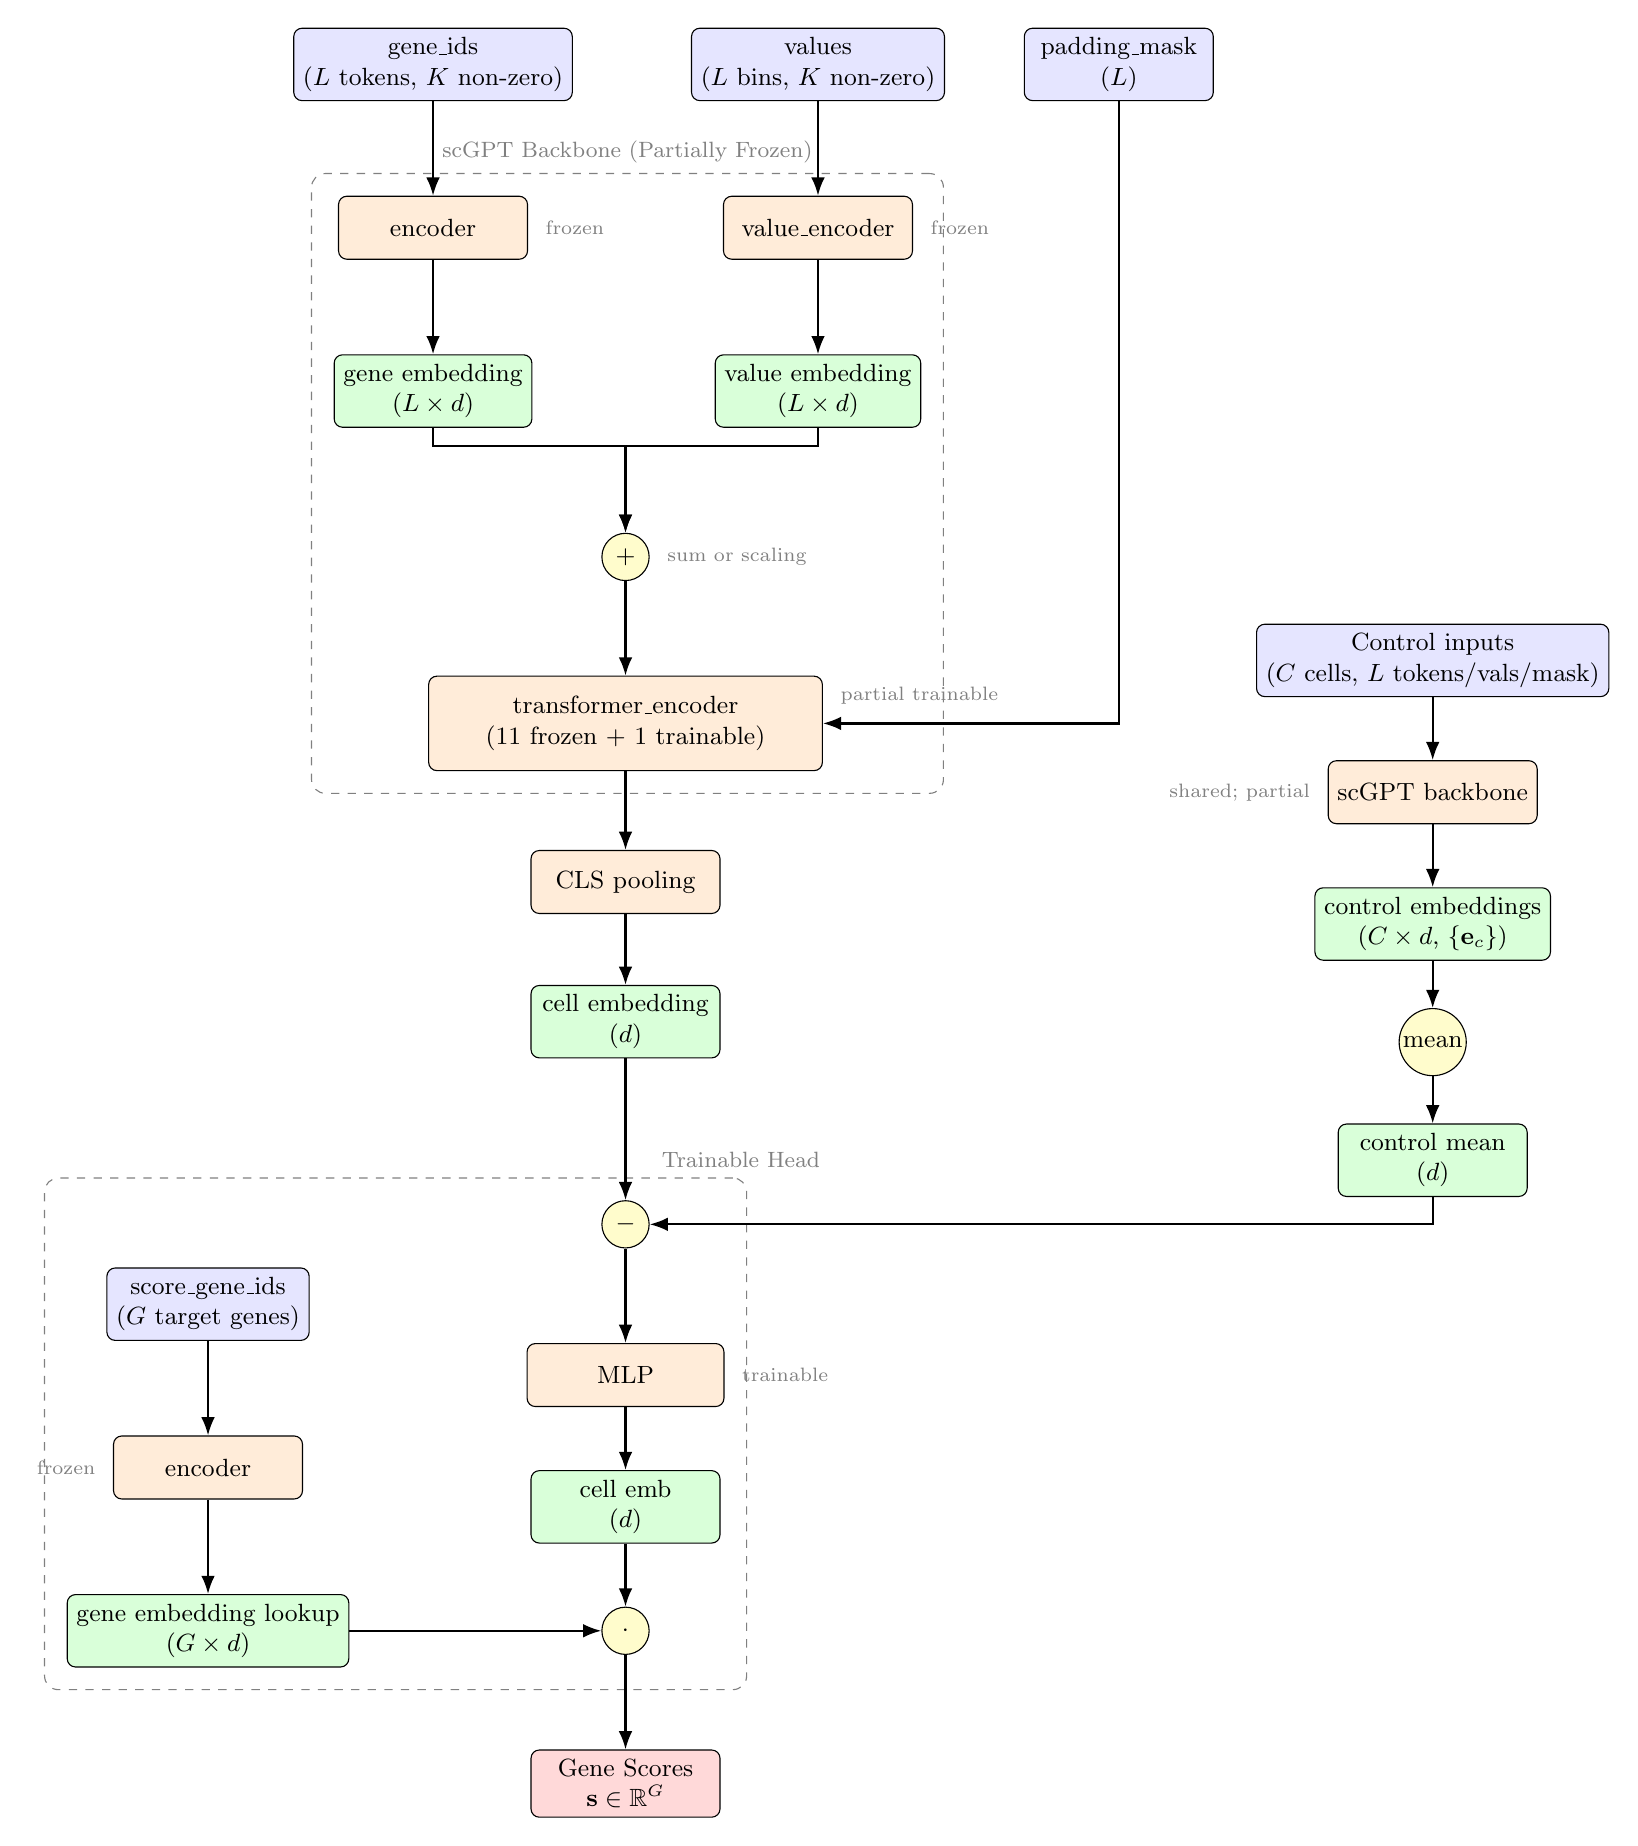
\begin{tikzpicture}[
    >=Latex,
    node distance=1.2cm and 2.4cm,
    font=\small,
    % Style definitions
    input/.style={draw, rounded corners=3pt, minimum width=2.4cm, minimum height=0.8cm, fill=blue!10, align=center},
    embed/.style={draw, rounded corners=3pt, minimum width=2.4cm, minimum height=0.8cm, fill=green!15, align=center},
    encoder/.style={draw, rounded corners=3pt, minimum width=2.4cm, minimum height=0.8cm, fill=orange!15, align=center},
    head/.style={draw, rounded corners=3pt, minimum width=2.4cm, minimum height=0.8cm, fill=yellow!15, align=center},
    unused/.style={draw, rounded corners=3pt, minimum width=2.4cm, minimum height=0.8cm, fill=gray!10, align=center, dashed},
    output/.style={draw, rounded corners=3pt, minimum width=2.4cm, minimum height=0.8cm, fill=red!15, align=center},
    operation/.style={circle, draw, minimum size=0.6cm, fill=yellow!20, inner sep=1pt},
    dashedbox/.style={draw, dashed, rounded corners=5pt, inner sep=8pt, gray},
    arrow/.style={->, thick, >=Latex, black},
]

%% ---------- INPUT LAYER ----------
\node[input] (gene_ids) {gene\_ids\\($L$ tokens, $K$ non-zero)};
\node[input, right=1.5cm of gene_ids] (values) {values\\($L$ bins, $K$ non-zero)};
\node[input, right=1cm of values] (padding) {padding\_mask\\($L$)};

%% ---------- ENCODERS + EMBEDDINGS (PARALLEL) ----------
\node[encoder, below=of gene_ids] (gene_encoder) {encoder};
\node[embed, below=of gene_encoder] (gene_emb) {gene embedding\\($L \times d$)};
\node[encoder, below=of values] (value_encoder) {value\_encoder};
\node[embed, below=of value_encoder] (value_emb) {value embedding\\($L \times d$)};

%% ---------- EMBEDDING FUSION ----------
\node[operation, below=1.8cm of $(gene_emb)!0.5!(value_emb)$] (add) {$+$};
\node[font=\scriptsize, gray, right=0.1cm of add.east] {sum or scaling};

%% ---------- TRANSFORMER ----------
\node[encoder, below=of add, minimum width=5cm, minimum height=1.2cm] (transformer) {transformer\_encoder\\(11 frozen + 1 trainable)};

%% ---------- OUTPUTS FROM TRANSFORMER ----------
\node[encoder, below=1.0cm of transformer] (cls_pool) {CLS pooling};
\node[embed, below=0.9cm of cls_pool] (cell_emb) {cell embedding\\($d$)};

%% ---------- CONTROL BRANCH ----------
\node[input, right=5.5cm of transformer, yshift=0.8cm] (control_branch) {Control inputs\\($C$ cells, $L$ tokens/vals/mask)};
\node[encoder, below=0.8cm of control_branch] (control_encoder) {scGPT backbone};
\node[embed, below=0.8cm of control_encoder] (control_emb) {control embeddings\\($C \times d$, $\{\mathbf{e}_c\}$)};
\node[operation, below=0.6cm of control_emb] (control_mean_op) {mean};
\node[embed, below=0.6cm of control_mean_op] (control_mean) {control mean\\($d$)};

%% ---------- DELTA EMBEDDING ----------
\node[operation, below=1.8cm of cell_emb] (subtract) {$-$};

%% ---------- GENE SCORING HEAD ----------
\node[encoder, below=of subtract, minimum width=2.5cm] (proj_mlp) {MLP};
\node[embed, below=0.8cm of proj_mlp] (cell_proj) {cell emb\\($d$)};
\node[operation, below=0.8cm of cell_proj] (dot_op) {$\cdot$};

%% ---------- OUTPUT ----------
\node[output, below=of dot_op] (scores) {Gene Scores\\$\mathbf{s} \in \mathbb{R}^{G}$};

%% ========== ARROWS ==========

% Inputs to encoders/embeddings
\draw[arrow] (gene_ids) -- (gene_encoder);
\draw[arrow] (gene_encoder) -- (gene_emb);
\draw[arrow] (values) -- (value_encoder);
\draw[arrow] (value_encoder) -- (value_emb);

% Embeddings to fusion (parallel)
\draw[arrow] (gene_emb) -- ++(0,-0.7) -| (add);
\draw[arrow] (value_emb) -- ++(0,-0.7) -| (add);

% Fusion to transformer
\draw[arrow] (add) -- (transformer);
\draw[arrow] (padding) |- (transformer);

% Transformer to cell embedding
\draw[arrow] (transformer.south) -- (cls_pool.north);
\draw[arrow] (cls_pool.south) -- (cell_emb.north);

% Control branch
\draw[arrow] (control_branch) -- (control_encoder);
\draw[arrow] (control_encoder) -- (control_emb);
\draw[arrow] (control_emb) -- (control_mean_op);
\draw[arrow] (control_mean_op) -- (control_mean);
\draw[arrow] (control_mean.south) |- (subtract.east);

% Cell embedding to delta
\draw[arrow] (cell_emb) -- (subtract);

% Delta to projection MLP
\draw[arrow] (subtract) -- (proj_mlp);
\draw[arrow] (proj_mlp) -- (cell_proj);
\draw[arrow] (cell_proj) -- (dot_op);

% Dot product to output
\draw[arrow] (dot_op) -- (scores);

% Gene embeddings to dot product (parallel flow)
\node[embed, left=3.2cm of dot_op] (gene_emb_lookup) {gene embedding lookup\\($G \times d$)};
\node[encoder, above=of gene_emb_lookup] (gene_emb_lookup_enc) {encoder};
\node[input, above=of gene_emb_lookup_enc] (score_gene_ids) {score\_gene\_ids\\($G$ target genes)};
\draw[arrow] (score_gene_ids) -- (gene_emb_lookup_enc);
\draw[arrow] (gene_emb_lookup_enc) -- (gene_emb_lookup);
\draw[arrow] (gene_emb_lookup.east) -- (dot_op.west);

%% ========== DASHED BOXES FOR GROUPING ==========

% scGPT Backbone box
\begin{scope}[on background layer]
    \node[dashedbox, fit=(gene_encoder)(value_encoder)(gene_emb)(value_emb)(add)(transformer), label={[font=\footnotesize, gray]above:scGPT Backbone (Partially Frozen)}] {};
\end{scope}

% Discriminative Head box
\begin{scope}[on background layer]
    \node[dashedbox, fit=(subtract)(proj_mlp)(cell_proj)(dot_op)(score_gene_ids)(gene_emb_lookup_enc)(gene_emb_lookup), label={[font=\footnotesize, gray]above right:Trainable Head}] {};
\end{scope}

%% ========== ANNOTATIONS ==========

% Trainability annotations
\node[font=\scriptsize, gray, right=0.1cm of gene_encoder.east] {frozen};
\node[font=\scriptsize, gray, right=0.1cm of value_encoder.east] {frozen};
\node[font=\scriptsize, gray, right=0.1cm of transformer.east, yshift=0.35cm] {partial trainable};
\node[font=\scriptsize, gray, left=0.1cm of control_encoder.west] {shared; partial};
\node[font=\scriptsize, gray, right=0.1cm of proj_mlp.east] {trainable};
\node[font=\scriptsize, gray, left=0.1cm of gene_emb_lookup_enc.west] {frozen};

\end{tikzpicture}
\ifexportfig
\else
\caption{Per-cell scGPT Discriminative Pipeline for Perturbation Gene Prediction.
For a single cell with $K$ non-zero genes, inputs are padded to length $L$.
Token IDs (\texttt{gene\_ids}), binned expression values, and a padding mask are fed to the scGPT backbone.
The \texttt{encoder} and \texttt{value\_encoder} produce gene/value embeddings, which are fused by element-wise addition (default)
or scaling (\texttt{input\_emb\_style}=\texttt{scaling}), then passed through \texttt{transformer\_encoder} to produce a CLS-based cell embedding.
A control branch runs the same backbone and the control mean is subtracted from the perturbed embedding.
The GeneScore head applies a projection MLP to the cell embedding before the dot product with the gene embedding lookup.
The \texttt{score\_gene\_ids} input is length $G$, the full set of candidate target genes, and its order defines the score output columns.
The backbone is partially frozen in this setup, with only the last transformer layer(s) and encoder norm optionally trainable.
Here, $G$ is the total number of genes in the dataset, $C$ is the number of control cells per perturbed cell, and $d$ is the embedding size.}
\label{fig:scgpt_pipeline}
\fi
\end{figure}

\end{document}
"
%   latex -interaction=nonstopmode -halt-on-error -jobname scGPT_pipeline_standalone_export -output-directory docs/report/final_report "\\def\\EXPORTFIG{1}\% scGPT Discriminative Pipeline Architecture (Standalone)
% Export (caption-free) SVG/PNG:
%   pdflatex -interaction=nonstopmode -halt-on-error -jobname scGPT_pipeline_standalone_export -output-directory docs/report/final_report "\\def\\EXPORTFIG{1}\\input{docs/report/final_report/scGPT_pipeline_standalone.tex}"
%   latex -interaction=nonstopmode -halt-on-error -jobname scGPT_pipeline_standalone_export -output-directory docs/report/final_report "\\def\\EXPORTFIG{1}\\input{docs/report/final_report/scGPT_pipeline_standalone.tex}"
%   dvisvgm --libgs=/opt/homebrew/lib/libgs.dylib -o docs/report/final_report/scGPT_pipeline_standalone.svg docs/report/final_report/scGPT_pipeline_standalone_export.dvi
%   gs -sDEVICE=pngalpha -r300 -o docs/report/final_report/scGPT_pipeline_standalone.png docs/report/final_report/scGPT_pipeline_standalone_export.pdf

\documentclass{article}
\usepackage[margin=1cm]{geometry}
\usepackage{tikz}
\usepackage{amsmath,amssymb}
\usetikzlibrary{arrows.meta, positioning, shapes.geometric, calc, fit, backgrounds}
\newif\ifexportfig
\ifdefined\EXPORTFIG
\exportfigtrue
\else
\exportfigfalse
\fi

\begin{document}
\pagecolor{white}

\begin{figure}[htbp]
\centering
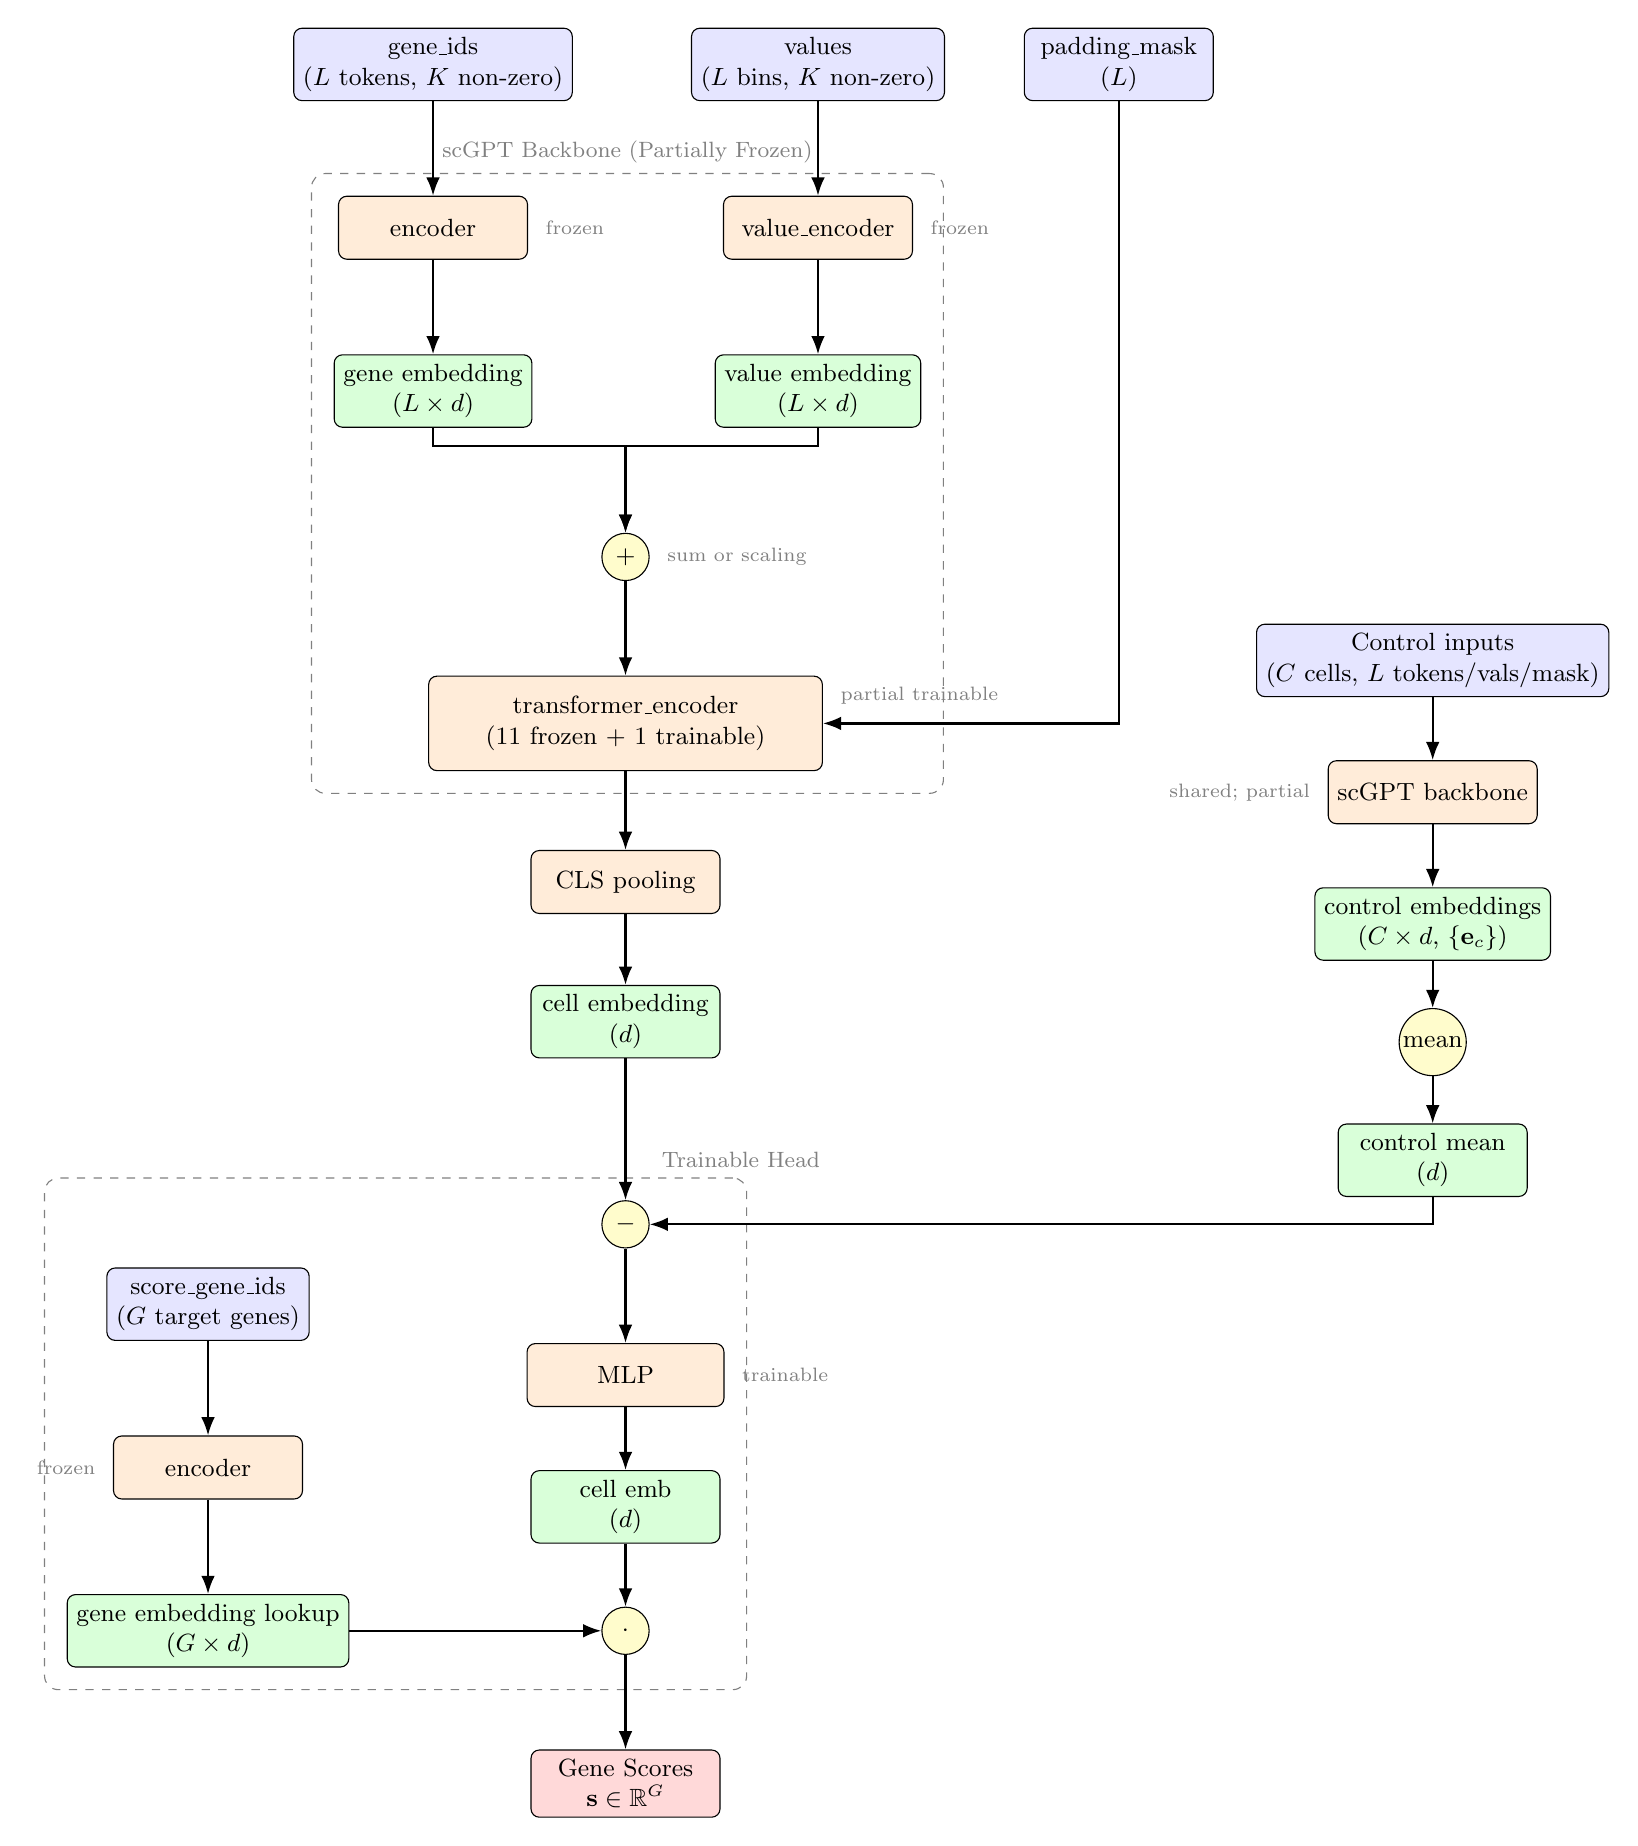
\begin{tikzpicture}[
    >=Latex,
    node distance=1.2cm and 2.4cm,
    font=\small,
    % Style definitions
    input/.style={draw, rounded corners=3pt, minimum width=2.4cm, minimum height=0.8cm, fill=blue!10, align=center},
    embed/.style={draw, rounded corners=3pt, minimum width=2.4cm, minimum height=0.8cm, fill=green!15, align=center},
    encoder/.style={draw, rounded corners=3pt, minimum width=2.4cm, minimum height=0.8cm, fill=orange!15, align=center},
    head/.style={draw, rounded corners=3pt, minimum width=2.4cm, minimum height=0.8cm, fill=yellow!15, align=center},
    unused/.style={draw, rounded corners=3pt, minimum width=2.4cm, minimum height=0.8cm, fill=gray!10, align=center, dashed},
    output/.style={draw, rounded corners=3pt, minimum width=2.4cm, minimum height=0.8cm, fill=red!15, align=center},
    operation/.style={circle, draw, minimum size=0.6cm, fill=yellow!20, inner sep=1pt},
    dashedbox/.style={draw, dashed, rounded corners=5pt, inner sep=8pt, gray},
    arrow/.style={->, thick, >=Latex, black},
]

%% ---------- INPUT LAYER ----------
\node[input] (gene_ids) {gene\_ids\\($L$ tokens, $K$ non-zero)};
\node[input, right=1.5cm of gene_ids] (values) {values\\($L$ bins, $K$ non-zero)};
\node[input, right=1cm of values] (padding) {padding\_mask\\($L$)};

%% ---------- ENCODERS + EMBEDDINGS (PARALLEL) ----------
\node[encoder, below=of gene_ids] (gene_encoder) {encoder};
\node[embed, below=of gene_encoder] (gene_emb) {gene embedding\\($L \times d$)};
\node[encoder, below=of values] (value_encoder) {value\_encoder};
\node[embed, below=of value_encoder] (value_emb) {value embedding\\($L \times d$)};

%% ---------- EMBEDDING FUSION ----------
\node[operation, below=1.8cm of $(gene_emb)!0.5!(value_emb)$] (add) {$+$};
\node[font=\scriptsize, gray, right=0.1cm of add.east] {sum or scaling};

%% ---------- TRANSFORMER ----------
\node[encoder, below=of add, minimum width=5cm, minimum height=1.2cm] (transformer) {transformer\_encoder\\(11 frozen + 1 trainable)};

%% ---------- OUTPUTS FROM TRANSFORMER ----------
\node[encoder, below=1.0cm of transformer] (cls_pool) {CLS pooling};
\node[embed, below=0.9cm of cls_pool] (cell_emb) {cell embedding\\($d$)};

%% ---------- CONTROL BRANCH ----------
\node[input, right=5.5cm of transformer, yshift=0.8cm] (control_branch) {Control inputs\\($C$ cells, $L$ tokens/vals/mask)};
\node[encoder, below=0.8cm of control_branch] (control_encoder) {scGPT backbone};
\node[embed, below=0.8cm of control_encoder] (control_emb) {control embeddings\\($C \times d$, $\{\mathbf{e}_c\}$)};
\node[operation, below=0.6cm of control_emb] (control_mean_op) {mean};
\node[embed, below=0.6cm of control_mean_op] (control_mean) {control mean\\($d$)};

%% ---------- DELTA EMBEDDING ----------
\node[operation, below=1.8cm of cell_emb] (subtract) {$-$};

%% ---------- GENE SCORING HEAD ----------
\node[encoder, below=of subtract, minimum width=2.5cm] (proj_mlp) {MLP};
\node[embed, below=0.8cm of proj_mlp] (cell_proj) {cell emb\\($d$)};
\node[operation, below=0.8cm of cell_proj] (dot_op) {$\cdot$};

%% ---------- OUTPUT ----------
\node[output, below=of dot_op] (scores) {Gene Scores\\$\mathbf{s} \in \mathbb{R}^{G}$};

%% ========== ARROWS ==========

% Inputs to encoders/embeddings
\draw[arrow] (gene_ids) -- (gene_encoder);
\draw[arrow] (gene_encoder) -- (gene_emb);
\draw[arrow] (values) -- (value_encoder);
\draw[arrow] (value_encoder) -- (value_emb);

% Embeddings to fusion (parallel)
\draw[arrow] (gene_emb) -- ++(0,-0.7) -| (add);
\draw[arrow] (value_emb) -- ++(0,-0.7) -| (add);

% Fusion to transformer
\draw[arrow] (add) -- (transformer);
\draw[arrow] (padding) |- (transformer);

% Transformer to cell embedding
\draw[arrow] (transformer.south) -- (cls_pool.north);
\draw[arrow] (cls_pool.south) -- (cell_emb.north);

% Control branch
\draw[arrow] (control_branch) -- (control_encoder);
\draw[arrow] (control_encoder) -- (control_emb);
\draw[arrow] (control_emb) -- (control_mean_op);
\draw[arrow] (control_mean_op) -- (control_mean);
\draw[arrow] (control_mean.south) |- (subtract.east);

% Cell embedding to delta
\draw[arrow] (cell_emb) -- (subtract);

% Delta to projection MLP
\draw[arrow] (subtract) -- (proj_mlp);
\draw[arrow] (proj_mlp) -- (cell_proj);
\draw[arrow] (cell_proj) -- (dot_op);

% Dot product to output
\draw[arrow] (dot_op) -- (scores);

% Gene embeddings to dot product (parallel flow)
\node[embed, left=3.2cm of dot_op] (gene_emb_lookup) {gene embedding lookup\\($G \times d$)};
\node[encoder, above=of gene_emb_lookup] (gene_emb_lookup_enc) {encoder};
\node[input, above=of gene_emb_lookup_enc] (score_gene_ids) {score\_gene\_ids\\($G$ target genes)};
\draw[arrow] (score_gene_ids) -- (gene_emb_lookup_enc);
\draw[arrow] (gene_emb_lookup_enc) -- (gene_emb_lookup);
\draw[arrow] (gene_emb_lookup.east) -- (dot_op.west);

%% ========== DASHED BOXES FOR GROUPING ==========

% scGPT Backbone box
\begin{scope}[on background layer]
    \node[dashedbox, fit=(gene_encoder)(value_encoder)(gene_emb)(value_emb)(add)(transformer), label={[font=\footnotesize, gray]above:scGPT Backbone (Partially Frozen)}] {};
\end{scope}

% Discriminative Head box
\begin{scope}[on background layer]
    \node[dashedbox, fit=(subtract)(proj_mlp)(cell_proj)(dot_op)(score_gene_ids)(gene_emb_lookup_enc)(gene_emb_lookup), label={[font=\footnotesize, gray]above right:Trainable Head}] {};
\end{scope}

%% ========== ANNOTATIONS ==========

% Trainability annotations
\node[font=\scriptsize, gray, right=0.1cm of gene_encoder.east] {frozen};
\node[font=\scriptsize, gray, right=0.1cm of value_encoder.east] {frozen};
\node[font=\scriptsize, gray, right=0.1cm of transformer.east, yshift=0.35cm] {partial trainable};
\node[font=\scriptsize, gray, left=0.1cm of control_encoder.west] {shared; partial};
\node[font=\scriptsize, gray, right=0.1cm of proj_mlp.east] {trainable};
\node[font=\scriptsize, gray, left=0.1cm of gene_emb_lookup_enc.west] {frozen};

\end{tikzpicture}
\ifexportfig
\else
\caption{Per-cell scGPT Discriminative Pipeline for Perturbation Gene Prediction.
For a single cell with $K$ non-zero genes, inputs are padded to length $L$.
Token IDs (\texttt{gene\_ids}), binned expression values, and a padding mask are fed to the scGPT backbone.
The \texttt{encoder} and \texttt{value\_encoder} produce gene/value embeddings, which are fused by element-wise addition (default)
or scaling (\texttt{input\_emb\_style}=\texttt{scaling}), then passed through \texttt{transformer\_encoder} to produce a CLS-based cell embedding.
A control branch runs the same backbone and the control mean is subtracted from the perturbed embedding.
The GeneScore head applies a projection MLP to the cell embedding before the dot product with the gene embedding lookup.
The \texttt{score\_gene\_ids} input is length $G$, the full set of candidate target genes, and its order defines the score output columns.
The backbone is partially frozen in this setup, with only the last transformer layer(s) and encoder norm optionally trainable.
Here, $G$ is the total number of genes in the dataset, $C$ is the number of control cells per perturbed cell, and $d$ is the embedding size.}
\label{fig:scgpt_pipeline}
\fi
\end{figure}

\end{document}
"
%   dvisvgm --libgs=/opt/homebrew/lib/libgs.dylib -o docs/report/final_report/scGPT_pipeline_standalone.svg docs/report/final_report/scGPT_pipeline_standalone_export.dvi
%   gs -sDEVICE=pngalpha -r300 -o docs/report/final_report/scGPT_pipeline_standalone.png docs/report/final_report/scGPT_pipeline_standalone_export.pdf

\documentclass{article}
\usepackage[margin=1cm]{geometry}
\usepackage{tikz}
\usepackage{amsmath,amssymb}
\usetikzlibrary{arrows.meta, positioning, shapes.geometric, calc, fit, backgrounds}
\newif\ifexportfig
\ifdefined\EXPORTFIG
\exportfigtrue
\else
\exportfigfalse
\fi

\begin{document}
\pagecolor{white}

\begin{figure}[htbp]
\centering
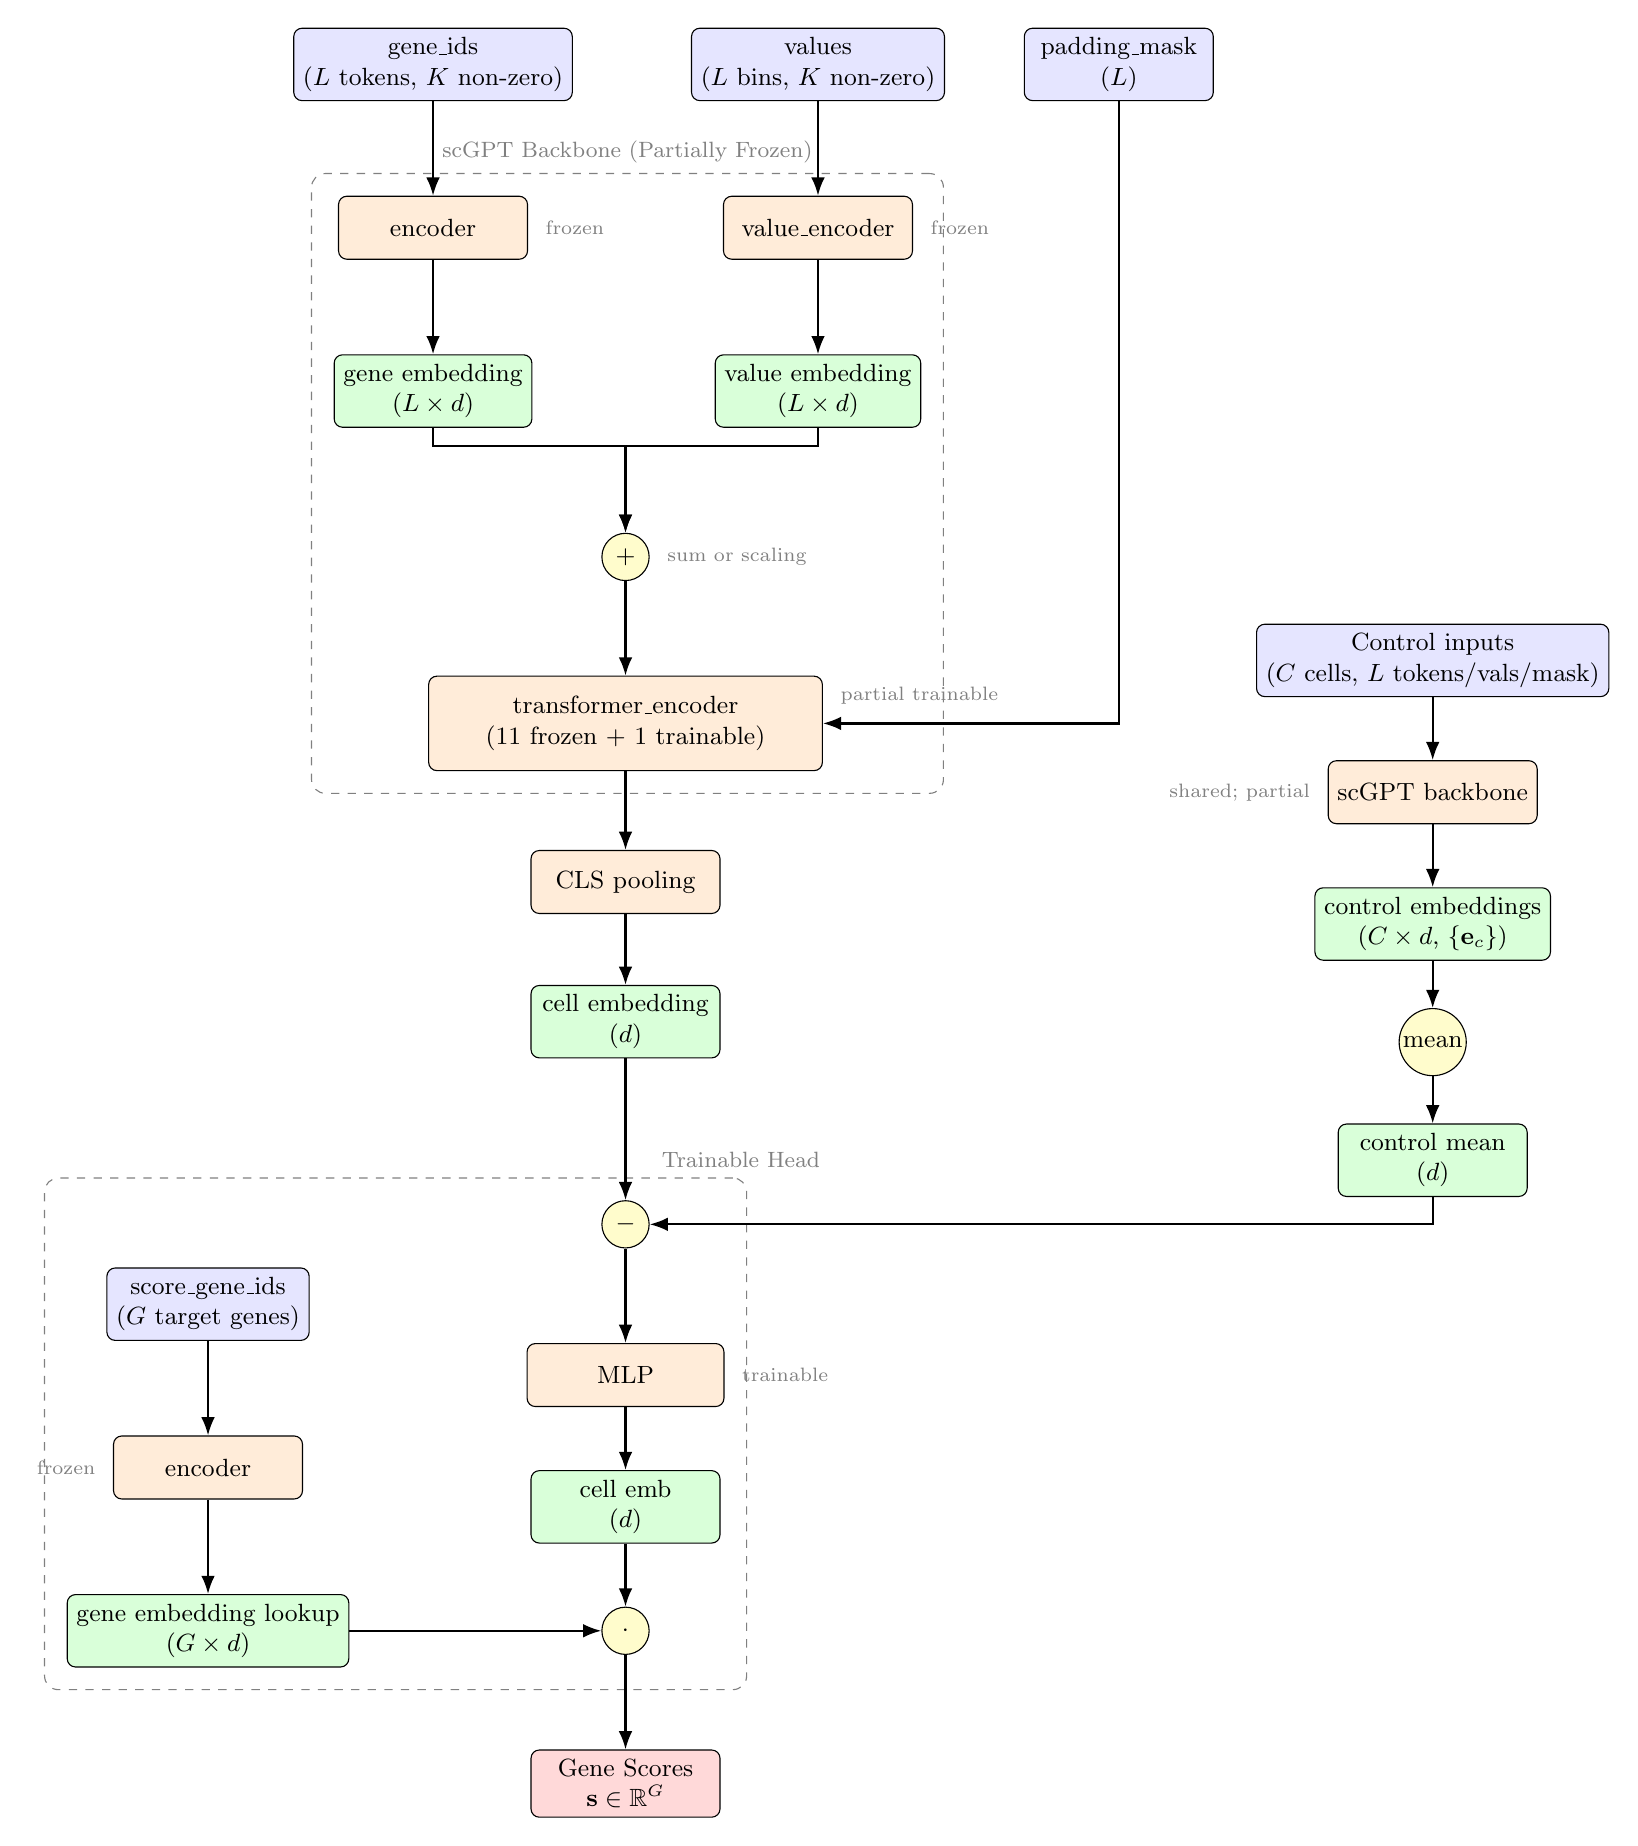
\begin{tikzpicture}[
    >=Latex,
    node distance=1.2cm and 2.4cm,
    font=\small,
    % Style definitions
    input/.style={draw, rounded corners=3pt, minimum width=2.4cm, minimum height=0.8cm, fill=blue!10, align=center},
    embed/.style={draw, rounded corners=3pt, minimum width=2.4cm, minimum height=0.8cm, fill=green!15, align=center},
    encoder/.style={draw, rounded corners=3pt, minimum width=2.4cm, minimum height=0.8cm, fill=orange!15, align=center},
    head/.style={draw, rounded corners=3pt, minimum width=2.4cm, minimum height=0.8cm, fill=yellow!15, align=center},
    unused/.style={draw, rounded corners=3pt, minimum width=2.4cm, minimum height=0.8cm, fill=gray!10, align=center, dashed},
    output/.style={draw, rounded corners=3pt, minimum width=2.4cm, minimum height=0.8cm, fill=red!15, align=center},
    operation/.style={circle, draw, minimum size=0.6cm, fill=yellow!20, inner sep=1pt},
    dashedbox/.style={draw, dashed, rounded corners=5pt, inner sep=8pt, gray},
    arrow/.style={->, thick, >=Latex, black},
]

%% ---------- INPUT LAYER ----------
\node[input] (gene_ids) {gene\_ids\\($L$ tokens, $K$ non-zero)};
\node[input, right=1.5cm of gene_ids] (values) {values\\($L$ bins, $K$ non-zero)};
\node[input, right=1cm of values] (padding) {padding\_mask\\($L$)};

%% ---------- ENCODERS + EMBEDDINGS (PARALLEL) ----------
\node[encoder, below=of gene_ids] (gene_encoder) {encoder};
\node[embed, below=of gene_encoder] (gene_emb) {gene embedding\\($L \times d$)};
\node[encoder, below=of values] (value_encoder) {value\_encoder};
\node[embed, below=of value_encoder] (value_emb) {value embedding\\($L \times d$)};

%% ---------- EMBEDDING FUSION ----------
\node[operation, below=1.8cm of $(gene_emb)!0.5!(value_emb)$] (add) {$+$};
\node[font=\scriptsize, gray, right=0.1cm of add.east] {sum or scaling};

%% ---------- TRANSFORMER ----------
\node[encoder, below=of add, minimum width=5cm, minimum height=1.2cm] (transformer) {transformer\_encoder\\(11 frozen + 1 trainable)};

%% ---------- OUTPUTS FROM TRANSFORMER ----------
\node[encoder, below=1.0cm of transformer] (cls_pool) {CLS pooling};
\node[embed, below=0.9cm of cls_pool] (cell_emb) {cell embedding\\($d$)};

%% ---------- CONTROL BRANCH ----------
\node[input, right=5.5cm of transformer, yshift=0.8cm] (control_branch) {Control inputs\\($C$ cells, $L$ tokens/vals/mask)};
\node[encoder, below=0.8cm of control_branch] (control_encoder) {scGPT backbone};
\node[embed, below=0.8cm of control_encoder] (control_emb) {control embeddings\\($C \times d$, $\{\mathbf{e}_c\}$)};
\node[operation, below=0.6cm of control_emb] (control_mean_op) {mean};
\node[embed, below=0.6cm of control_mean_op] (control_mean) {control mean\\($d$)};

%% ---------- DELTA EMBEDDING ----------
\node[operation, below=1.8cm of cell_emb] (subtract) {$-$};

%% ---------- GENE SCORING HEAD ----------
\node[encoder, below=of subtract, minimum width=2.5cm] (proj_mlp) {MLP};
\node[embed, below=0.8cm of proj_mlp] (cell_proj) {cell emb\\($d$)};
\node[operation, below=0.8cm of cell_proj] (dot_op) {$\cdot$};

%% ---------- OUTPUT ----------
\node[output, below=of dot_op] (scores) {Gene Scores\\$\mathbf{s} \in \mathbb{R}^{G}$};

%% ========== ARROWS ==========

% Inputs to encoders/embeddings
\draw[arrow] (gene_ids) -- (gene_encoder);
\draw[arrow] (gene_encoder) -- (gene_emb);
\draw[arrow] (values) -- (value_encoder);
\draw[arrow] (value_encoder) -- (value_emb);

% Embeddings to fusion (parallel)
\draw[arrow] (gene_emb) -- ++(0,-0.7) -| (add);
\draw[arrow] (value_emb) -- ++(0,-0.7) -| (add);

% Fusion to transformer
\draw[arrow] (add) -- (transformer);
\draw[arrow] (padding) |- (transformer);

% Transformer to cell embedding
\draw[arrow] (transformer.south) -- (cls_pool.north);
\draw[arrow] (cls_pool.south) -- (cell_emb.north);

% Control branch
\draw[arrow] (control_branch) -- (control_encoder);
\draw[arrow] (control_encoder) -- (control_emb);
\draw[arrow] (control_emb) -- (control_mean_op);
\draw[arrow] (control_mean_op) -- (control_mean);
\draw[arrow] (control_mean.south) |- (subtract.east);

% Cell embedding to delta
\draw[arrow] (cell_emb) -- (subtract);

% Delta to projection MLP
\draw[arrow] (subtract) -- (proj_mlp);
\draw[arrow] (proj_mlp) -- (cell_proj);
\draw[arrow] (cell_proj) -- (dot_op);

% Dot product to output
\draw[arrow] (dot_op) -- (scores);

% Gene embeddings to dot product (parallel flow)
\node[embed, left=3.2cm of dot_op] (gene_emb_lookup) {gene embedding lookup\\($G \times d$)};
\node[encoder, above=of gene_emb_lookup] (gene_emb_lookup_enc) {encoder};
\node[input, above=of gene_emb_lookup_enc] (score_gene_ids) {score\_gene\_ids\\($G$ target genes)};
\draw[arrow] (score_gene_ids) -- (gene_emb_lookup_enc);
\draw[arrow] (gene_emb_lookup_enc) -- (gene_emb_lookup);
\draw[arrow] (gene_emb_lookup.east) -- (dot_op.west);

%% ========== DASHED BOXES FOR GROUPING ==========

% scGPT Backbone box
\begin{scope}[on background layer]
    \node[dashedbox, fit=(gene_encoder)(value_encoder)(gene_emb)(value_emb)(add)(transformer), label={[font=\footnotesize, gray]above:scGPT Backbone (Partially Frozen)}] {};
\end{scope}

% Discriminative Head box
\begin{scope}[on background layer]
    \node[dashedbox, fit=(subtract)(proj_mlp)(cell_proj)(dot_op)(score_gene_ids)(gene_emb_lookup_enc)(gene_emb_lookup), label={[font=\footnotesize, gray]above right:Trainable Head}] {};
\end{scope}

%% ========== ANNOTATIONS ==========

% Trainability annotations
\node[font=\scriptsize, gray, right=0.1cm of gene_encoder.east] {frozen};
\node[font=\scriptsize, gray, right=0.1cm of value_encoder.east] {frozen};
\node[font=\scriptsize, gray, right=0.1cm of transformer.east, yshift=0.35cm] {partial trainable};
\node[font=\scriptsize, gray, left=0.1cm of control_encoder.west] {shared; partial};
\node[font=\scriptsize, gray, right=0.1cm of proj_mlp.east] {trainable};
\node[font=\scriptsize, gray, left=0.1cm of gene_emb_lookup_enc.west] {frozen};

\end{tikzpicture}
\ifexportfig
\else
\caption{Per-cell scGPT Discriminative Pipeline for Perturbation Gene Prediction.
For a single cell with $K$ non-zero genes, inputs are padded to length $L$.
Token IDs (\texttt{gene\_ids}), binned expression values, and a padding mask are fed to the scGPT backbone.
The \texttt{encoder} and \texttt{value\_encoder} produce gene/value embeddings, which are fused by element-wise addition (default)
or scaling (\texttt{input\_emb\_style}=\texttt{scaling}), then passed through \texttt{transformer\_encoder} to produce a CLS-based cell embedding.
A control branch runs the same backbone and the control mean is subtracted from the perturbed embedding.
The GeneScore head applies a projection MLP to the cell embedding before the dot product with the gene embedding lookup.
The \texttt{score\_gene\_ids} input is length $G$, the full set of candidate target genes, and its order defines the score output columns.
The backbone is partially frozen in this setup, with only the last transformer layer(s) and encoder norm optionally trainable.
Here, $G$ is the total number of genes in the dataset, $C$ is the number of control cells per perturbed cell, and $d$ is the embedding size.}
\label{fig:scgpt_pipeline}
\fi
\end{figure}

\end{document}
"
%   dvisvgm --libgs=/opt/homebrew/lib/libgs.dylib -o docs/report/final_report/scGPT_pipeline_standalone.svg docs/report/final_report/scGPT_pipeline_standalone_export.dvi
%   gs -sDEVICE=pngalpha -r300 -o docs/report/final_report/scGPT_pipeline_standalone.png docs/report/final_report/scGPT_pipeline_standalone_export.pdf

\documentclass{article}
\usepackage[margin=1cm]{geometry}
\usepackage{tikz}
\usepackage{amsmath,amssymb}
\usetikzlibrary{arrows.meta, positioning, shapes.geometric, calc, fit, backgrounds}
\newif\ifexportfig
\ifdefined\EXPORTFIG
\exportfigtrue
\else
\exportfigfalse
\fi

\begin{document}
\pagecolor{white}

\begin{figure}[htbp]
\centering
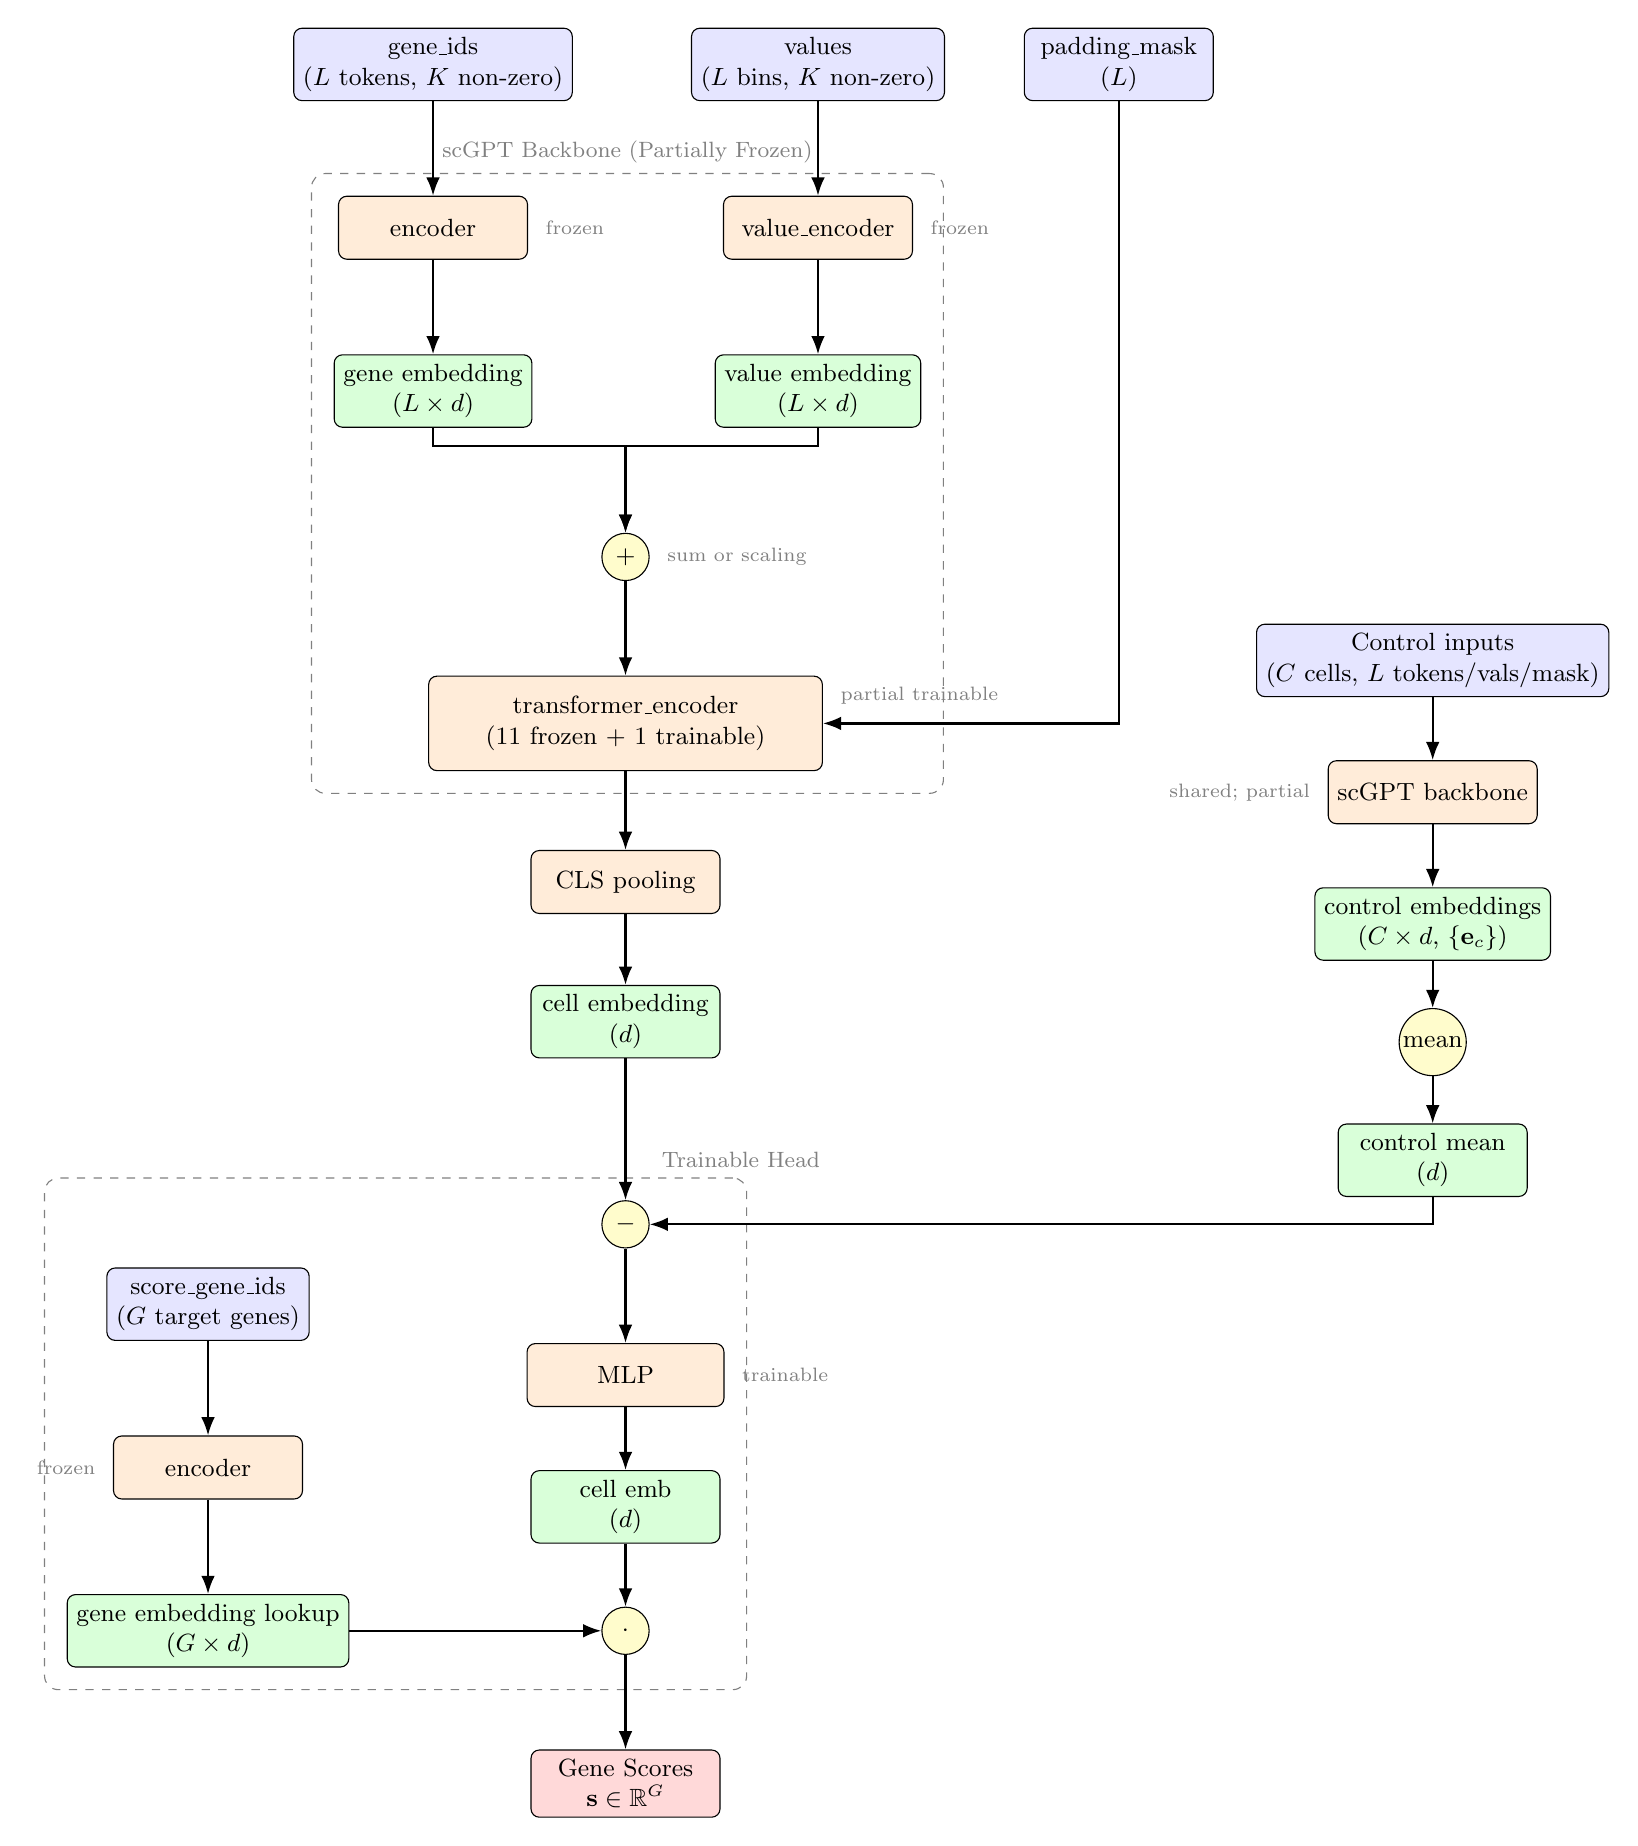
\begin{tikzpicture}[
    >=Latex,
    node distance=1.2cm and 2.4cm,
    font=\small,
    % Style definitions
    input/.style={draw, rounded corners=3pt, minimum width=2.4cm, minimum height=0.8cm, fill=blue!10, align=center},
    embed/.style={draw, rounded corners=3pt, minimum width=2.4cm, minimum height=0.8cm, fill=green!15, align=center},
    encoder/.style={draw, rounded corners=3pt, minimum width=2.4cm, minimum height=0.8cm, fill=orange!15, align=center},
    head/.style={draw, rounded corners=3pt, minimum width=2.4cm, minimum height=0.8cm, fill=yellow!15, align=center},
    unused/.style={draw, rounded corners=3pt, minimum width=2.4cm, minimum height=0.8cm, fill=gray!10, align=center, dashed},
    output/.style={draw, rounded corners=3pt, minimum width=2.4cm, minimum height=0.8cm, fill=red!15, align=center},
    operation/.style={circle, draw, minimum size=0.6cm, fill=yellow!20, inner sep=1pt},
    dashedbox/.style={draw, dashed, rounded corners=5pt, inner sep=8pt, gray},
    arrow/.style={->, thick, >=Latex, black},
]

%% ---------- INPUT LAYER ----------
\node[input] (gene_ids) {gene\_ids\\($L$ tokens, $K$ non-zero)};
\node[input, right=1.5cm of gene_ids] (values) {values\\($L$ bins, $K$ non-zero)};
\node[input, right=1cm of values] (padding) {padding\_mask\\($L$)};

%% ---------- ENCODERS + EMBEDDINGS (PARALLEL) ----------
\node[encoder, below=of gene_ids] (gene_encoder) {encoder};
\node[embed, below=of gene_encoder] (gene_emb) {gene embedding\\($L \times d$)};
\node[encoder, below=of values] (value_encoder) {value\_encoder};
\node[embed, below=of value_encoder] (value_emb) {value embedding\\($L \times d$)};

%% ---------- EMBEDDING FUSION ----------
\node[operation, below=1.8cm of $(gene_emb)!0.5!(value_emb)$] (add) {$+$};
\node[font=\scriptsize, gray, right=0.1cm of add.east] {sum or scaling};

%% ---------- TRANSFORMER ----------
\node[encoder, below=of add, minimum width=5cm, minimum height=1.2cm] (transformer) {transformer\_encoder\\(11 frozen + 1 trainable)};

%% ---------- OUTPUTS FROM TRANSFORMER ----------
\node[encoder, below=1.0cm of transformer] (cls_pool) {CLS pooling};
\node[embed, below=0.9cm of cls_pool] (cell_emb) {cell embedding\\($d$)};

%% ---------- CONTROL BRANCH ----------
\node[input, right=5.5cm of transformer, yshift=0.8cm] (control_branch) {Control inputs\\($C$ cells, $L$ tokens/vals/mask)};
\node[encoder, below=0.8cm of control_branch] (control_encoder) {scGPT backbone};
\node[embed, below=0.8cm of control_encoder] (control_emb) {control embeddings\\($C \times d$, $\{\mathbf{e}_c\}$)};
\node[operation, below=0.6cm of control_emb] (control_mean_op) {mean};
\node[embed, below=0.6cm of control_mean_op] (control_mean) {control mean\\($d$)};

%% ---------- DELTA EMBEDDING ----------
\node[operation, below=1.8cm of cell_emb] (subtract) {$-$};

%% ---------- GENE SCORING HEAD ----------
\node[encoder, below=of subtract, minimum width=2.5cm] (proj_mlp) {MLP};
\node[embed, below=0.8cm of proj_mlp] (cell_proj) {cell emb\\($d$)};
\node[operation, below=0.8cm of cell_proj] (dot_op) {$\cdot$};

%% ---------- OUTPUT ----------
\node[output, below=of dot_op] (scores) {Gene Scores\\$\mathbf{s} \in \mathbb{R}^{G}$};

%% ========== ARROWS ==========

% Inputs to encoders/embeddings
\draw[arrow] (gene_ids) -- (gene_encoder);
\draw[arrow] (gene_encoder) -- (gene_emb);
\draw[arrow] (values) -- (value_encoder);
\draw[arrow] (value_encoder) -- (value_emb);

% Embeddings to fusion (parallel)
\draw[arrow] (gene_emb) -- ++(0,-0.7) -| (add);
\draw[arrow] (value_emb) -- ++(0,-0.7) -| (add);

% Fusion to transformer
\draw[arrow] (add) -- (transformer);
\draw[arrow] (padding) |- (transformer);

% Transformer to cell embedding
\draw[arrow] (transformer.south) -- (cls_pool.north);
\draw[arrow] (cls_pool.south) -- (cell_emb.north);

% Control branch
\draw[arrow] (control_branch) -- (control_encoder);
\draw[arrow] (control_encoder) -- (control_emb);
\draw[arrow] (control_emb) -- (control_mean_op);
\draw[arrow] (control_mean_op) -- (control_mean);
\draw[arrow] (control_mean.south) |- (subtract.east);

% Cell embedding to delta
\draw[arrow] (cell_emb) -- (subtract);

% Delta to projection MLP
\draw[arrow] (subtract) -- (proj_mlp);
\draw[arrow] (proj_mlp) -- (cell_proj);
\draw[arrow] (cell_proj) -- (dot_op);

% Dot product to output
\draw[arrow] (dot_op) -- (scores);

% Gene embeddings to dot product (parallel flow)
\node[embed, left=3.2cm of dot_op] (gene_emb_lookup) {gene embedding lookup\\($G \times d$)};
\node[encoder, above=of gene_emb_lookup] (gene_emb_lookup_enc) {encoder};
\node[input, above=of gene_emb_lookup_enc] (score_gene_ids) {score\_gene\_ids\\($G$ target genes)};
\draw[arrow] (score_gene_ids) -- (gene_emb_lookup_enc);
\draw[arrow] (gene_emb_lookup_enc) -- (gene_emb_lookup);
\draw[arrow] (gene_emb_lookup.east) -- (dot_op.west);

%% ========== DASHED BOXES FOR GROUPING ==========

% scGPT Backbone box
\begin{scope}[on background layer]
    \node[dashedbox, fit=(gene_encoder)(value_encoder)(gene_emb)(value_emb)(add)(transformer), label={[font=\footnotesize, gray]above:scGPT Backbone (Partially Frozen)}] {};
\end{scope}

% Discriminative Head box
\begin{scope}[on background layer]
    \node[dashedbox, fit=(subtract)(proj_mlp)(cell_proj)(dot_op)(score_gene_ids)(gene_emb_lookup_enc)(gene_emb_lookup), label={[font=\footnotesize, gray]above right:Trainable Head}] {};
\end{scope}

%% ========== ANNOTATIONS ==========

% Trainability annotations
\node[font=\scriptsize, gray, right=0.1cm of gene_encoder.east] {frozen};
\node[font=\scriptsize, gray, right=0.1cm of value_encoder.east] {frozen};
\node[font=\scriptsize, gray, right=0.1cm of transformer.east, yshift=0.35cm] {partial trainable};
\node[font=\scriptsize, gray, left=0.1cm of control_encoder.west] {shared; partial};
\node[font=\scriptsize, gray, right=0.1cm of proj_mlp.east] {trainable};
\node[font=\scriptsize, gray, left=0.1cm of gene_emb_lookup_enc.west] {frozen};

\end{tikzpicture}
\ifexportfig
\else
\caption{Per-cell scGPT Discriminative Pipeline for Perturbation Gene Prediction.
For a single cell with $K$ non-zero genes, inputs are padded to length $L$.
Token IDs (\texttt{gene\_ids}), binned expression values, and a padding mask are fed to the scGPT backbone.
The \texttt{encoder} and \texttt{value\_encoder} produce gene/value embeddings, which are fused by element-wise addition (default)
or scaling (\texttt{input\_emb\_style}=\texttt{scaling}), then passed through \texttt{transformer\_encoder} to produce a CLS-based cell embedding.
A control branch runs the same backbone and the control mean is subtracted from the perturbed embedding.
The GeneScore head applies a projection MLP to the cell embedding before the dot product with the gene embedding lookup.
The \texttt{score\_gene\_ids} input is length $G$, the full set of candidate target genes, and its order defines the score output columns.
The backbone is partially frozen in this setup, with only the last transformer layer(s) and encoder norm optionally trainable.
Here, $G$ is the total number of genes in the dataset, $C$ is the number of control cells per perturbed cell, and $d$ is the embedding size.}
\label{fig:scgpt_pipeline}
\fi
\end{figure}

\end{document}
"
%   latex -interaction=nonstopmode -halt-on-error -jobname scGPT_pipeline_standalone_export -output-directory docs/report/final_report "\\def\\EXPORTFIG{1}\% scGPT Discriminative Pipeline Architecture (Standalone)
% Export (caption-free) SVG/PNG:
%   pdflatex -interaction=nonstopmode -halt-on-error -jobname scGPT_pipeline_standalone_export -output-directory docs/report/final_report "\\def\\EXPORTFIG{1}\% scGPT Discriminative Pipeline Architecture (Standalone)
% Export (caption-free) SVG/PNG:
%   pdflatex -interaction=nonstopmode -halt-on-error -jobname scGPT_pipeline_standalone_export -output-directory docs/report/final_report "\\def\\EXPORTFIG{1}\% scGPT Discriminative Pipeline Architecture (Standalone)
% Export (caption-free) SVG/PNG:
%   pdflatex -interaction=nonstopmode -halt-on-error -jobname scGPT_pipeline_standalone_export -output-directory docs/report/final_report "\\def\\EXPORTFIG{1}\\input{docs/report/final_report/scGPT_pipeline_standalone.tex}"
%   latex -interaction=nonstopmode -halt-on-error -jobname scGPT_pipeline_standalone_export -output-directory docs/report/final_report "\\def\\EXPORTFIG{1}\\input{docs/report/final_report/scGPT_pipeline_standalone.tex}"
%   dvisvgm --libgs=/opt/homebrew/lib/libgs.dylib -o docs/report/final_report/scGPT_pipeline_standalone.svg docs/report/final_report/scGPT_pipeline_standalone_export.dvi
%   gs -sDEVICE=pngalpha -r300 -o docs/report/final_report/scGPT_pipeline_standalone.png docs/report/final_report/scGPT_pipeline_standalone_export.pdf

\documentclass{article}
\usepackage[margin=1cm]{geometry}
\usepackage{tikz}
\usepackage{amsmath,amssymb}
\usetikzlibrary{arrows.meta, positioning, shapes.geometric, calc, fit, backgrounds}
\newif\ifexportfig
\ifdefined\EXPORTFIG
\exportfigtrue
\else
\exportfigfalse
\fi

\begin{document}
\pagecolor{white}

\begin{figure}[htbp]
\centering
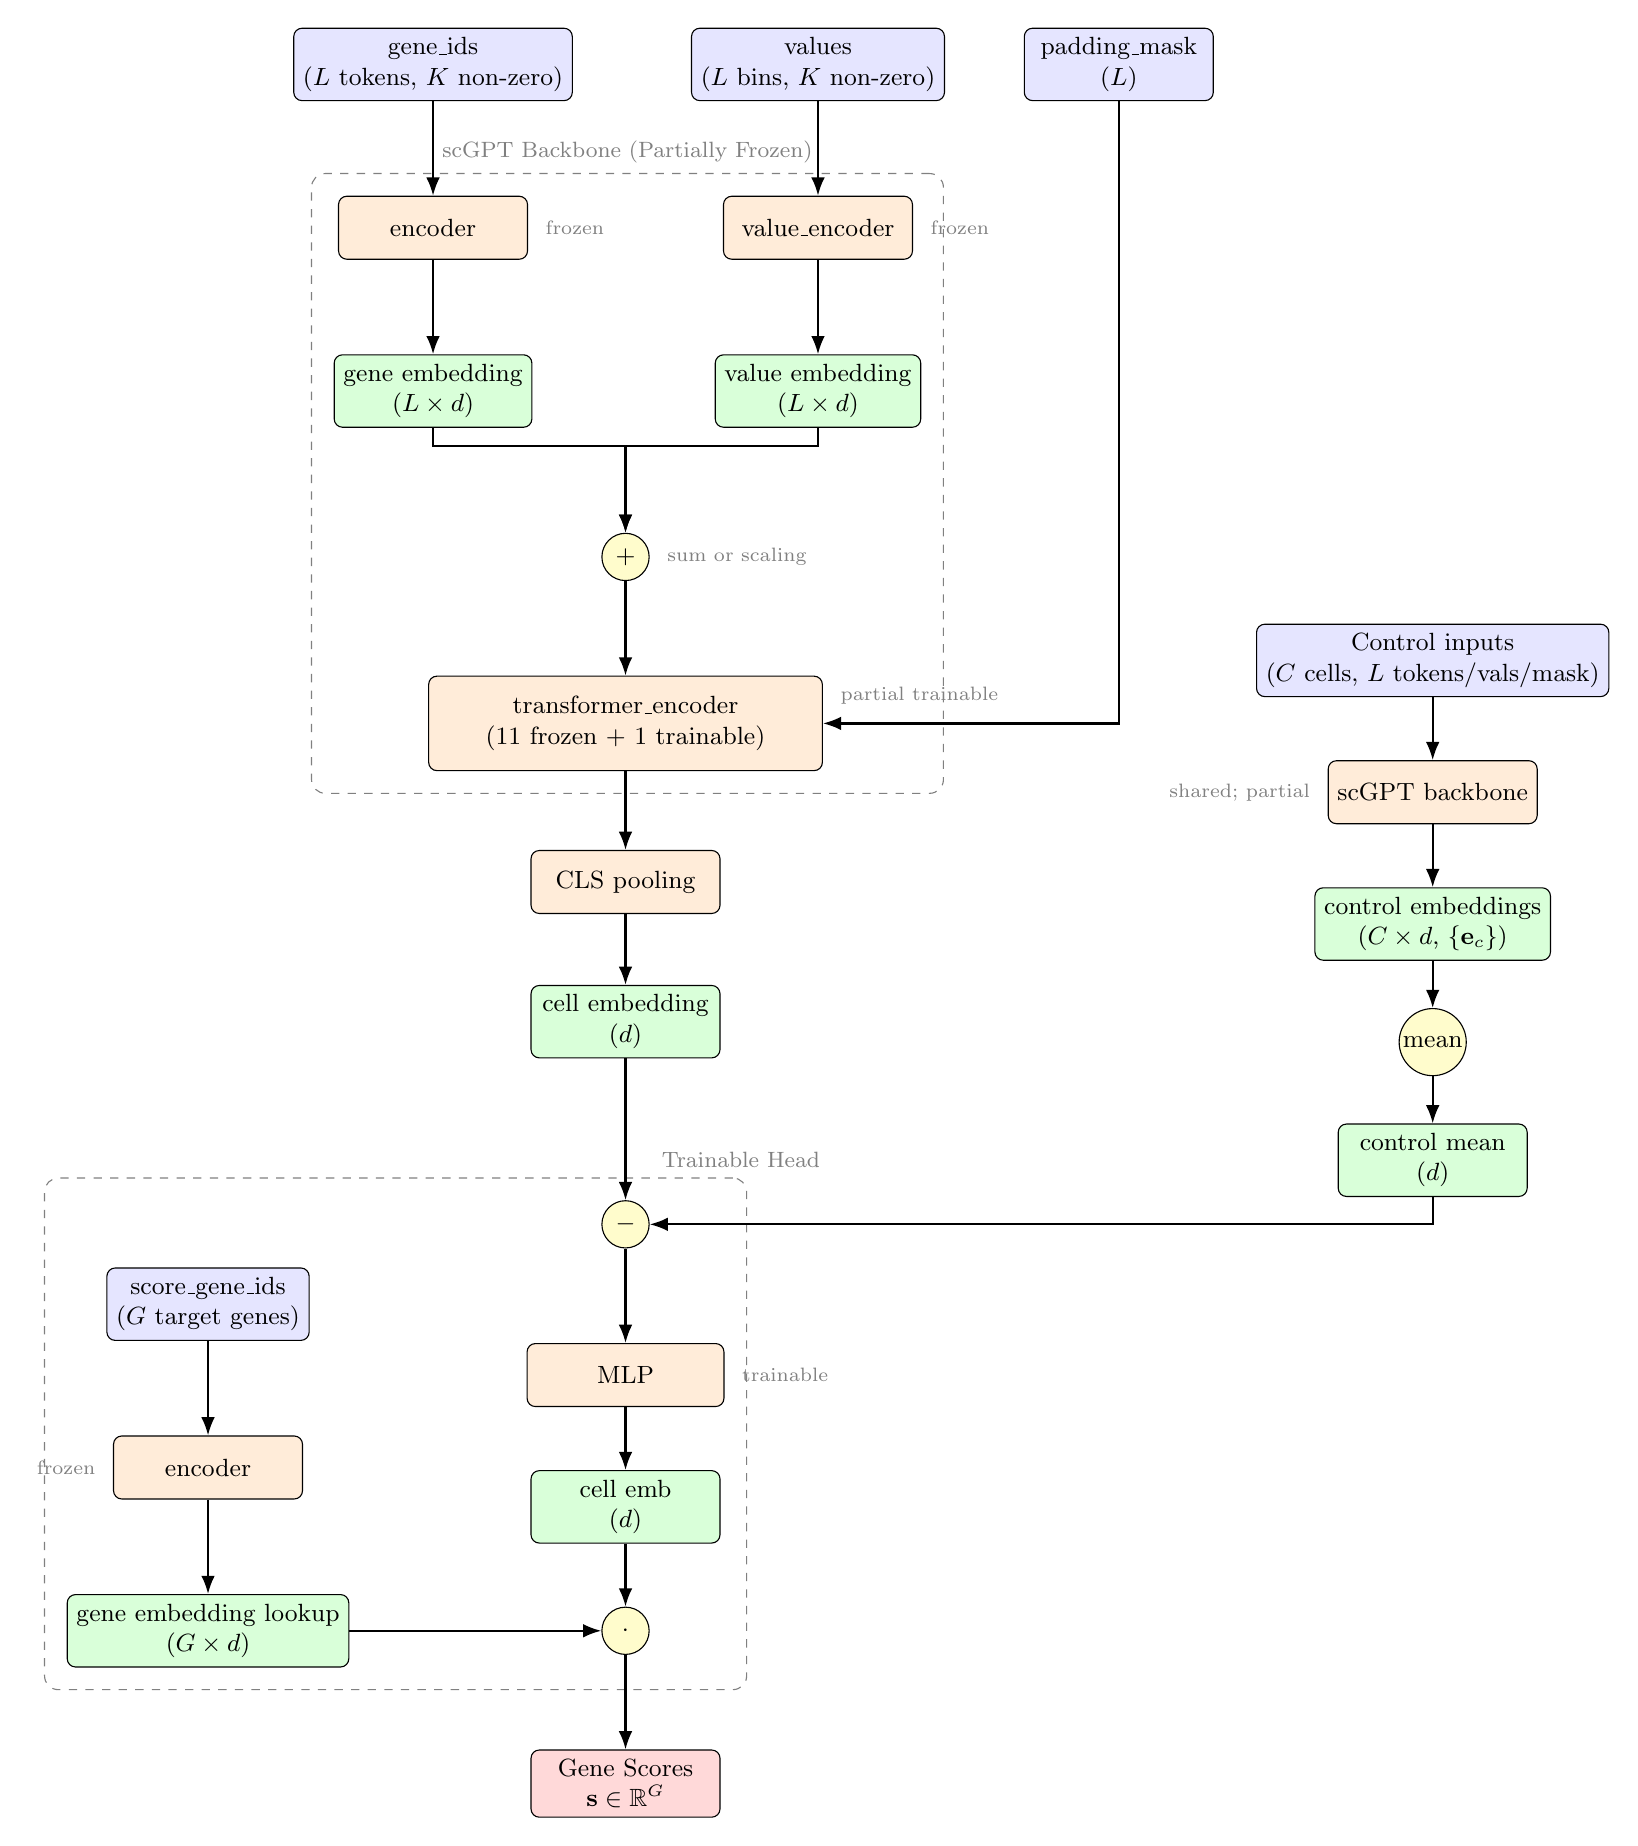
\begin{tikzpicture}[
    >=Latex,
    node distance=1.2cm and 2.4cm,
    font=\small,
    % Style definitions
    input/.style={draw, rounded corners=3pt, minimum width=2.4cm, minimum height=0.8cm, fill=blue!10, align=center},
    embed/.style={draw, rounded corners=3pt, minimum width=2.4cm, minimum height=0.8cm, fill=green!15, align=center},
    encoder/.style={draw, rounded corners=3pt, minimum width=2.4cm, minimum height=0.8cm, fill=orange!15, align=center},
    head/.style={draw, rounded corners=3pt, minimum width=2.4cm, minimum height=0.8cm, fill=yellow!15, align=center},
    unused/.style={draw, rounded corners=3pt, minimum width=2.4cm, minimum height=0.8cm, fill=gray!10, align=center, dashed},
    output/.style={draw, rounded corners=3pt, minimum width=2.4cm, minimum height=0.8cm, fill=red!15, align=center},
    operation/.style={circle, draw, minimum size=0.6cm, fill=yellow!20, inner sep=1pt},
    dashedbox/.style={draw, dashed, rounded corners=5pt, inner sep=8pt, gray},
    arrow/.style={->, thick, >=Latex, black},
]

%% ---------- INPUT LAYER ----------
\node[input] (gene_ids) {gene\_ids\\($L$ tokens, $K$ non-zero)};
\node[input, right=1.5cm of gene_ids] (values) {values\\($L$ bins, $K$ non-zero)};
\node[input, right=1cm of values] (padding) {padding\_mask\\($L$)};

%% ---------- ENCODERS + EMBEDDINGS (PARALLEL) ----------
\node[encoder, below=of gene_ids] (gene_encoder) {encoder};
\node[embed, below=of gene_encoder] (gene_emb) {gene embedding\\($L \times d$)};
\node[encoder, below=of values] (value_encoder) {value\_encoder};
\node[embed, below=of value_encoder] (value_emb) {value embedding\\($L \times d$)};

%% ---------- EMBEDDING FUSION ----------
\node[operation, below=1.8cm of $(gene_emb)!0.5!(value_emb)$] (add) {$+$};
\node[font=\scriptsize, gray, right=0.1cm of add.east] {sum or scaling};

%% ---------- TRANSFORMER ----------
\node[encoder, below=of add, minimum width=5cm, minimum height=1.2cm] (transformer) {transformer\_encoder\\(11 frozen + 1 trainable)};

%% ---------- OUTPUTS FROM TRANSFORMER ----------
\node[encoder, below=1.0cm of transformer] (cls_pool) {CLS pooling};
\node[embed, below=0.9cm of cls_pool] (cell_emb) {cell embedding\\($d$)};

%% ---------- CONTROL BRANCH ----------
\node[input, right=5.5cm of transformer, yshift=0.8cm] (control_branch) {Control inputs\\($C$ cells, $L$ tokens/vals/mask)};
\node[encoder, below=0.8cm of control_branch] (control_encoder) {scGPT backbone};
\node[embed, below=0.8cm of control_encoder] (control_emb) {control embeddings\\($C \times d$, $\{\mathbf{e}_c\}$)};
\node[operation, below=0.6cm of control_emb] (control_mean_op) {mean};
\node[embed, below=0.6cm of control_mean_op] (control_mean) {control mean\\($d$)};

%% ---------- DELTA EMBEDDING ----------
\node[operation, below=1.8cm of cell_emb] (subtract) {$-$};

%% ---------- GENE SCORING HEAD ----------
\node[encoder, below=of subtract, minimum width=2.5cm] (proj_mlp) {MLP};
\node[embed, below=0.8cm of proj_mlp] (cell_proj) {cell emb\\($d$)};
\node[operation, below=0.8cm of cell_proj] (dot_op) {$\cdot$};

%% ---------- OUTPUT ----------
\node[output, below=of dot_op] (scores) {Gene Scores\\$\mathbf{s} \in \mathbb{R}^{G}$};

%% ========== ARROWS ==========

% Inputs to encoders/embeddings
\draw[arrow] (gene_ids) -- (gene_encoder);
\draw[arrow] (gene_encoder) -- (gene_emb);
\draw[arrow] (values) -- (value_encoder);
\draw[arrow] (value_encoder) -- (value_emb);

% Embeddings to fusion (parallel)
\draw[arrow] (gene_emb) -- ++(0,-0.7) -| (add);
\draw[arrow] (value_emb) -- ++(0,-0.7) -| (add);

% Fusion to transformer
\draw[arrow] (add) -- (transformer);
\draw[arrow] (padding) |- (transformer);

% Transformer to cell embedding
\draw[arrow] (transformer.south) -- (cls_pool.north);
\draw[arrow] (cls_pool.south) -- (cell_emb.north);

% Control branch
\draw[arrow] (control_branch) -- (control_encoder);
\draw[arrow] (control_encoder) -- (control_emb);
\draw[arrow] (control_emb) -- (control_mean_op);
\draw[arrow] (control_mean_op) -- (control_mean);
\draw[arrow] (control_mean.south) |- (subtract.east);

% Cell embedding to delta
\draw[arrow] (cell_emb) -- (subtract);

% Delta to projection MLP
\draw[arrow] (subtract) -- (proj_mlp);
\draw[arrow] (proj_mlp) -- (cell_proj);
\draw[arrow] (cell_proj) -- (dot_op);

% Dot product to output
\draw[arrow] (dot_op) -- (scores);

% Gene embeddings to dot product (parallel flow)
\node[embed, left=3.2cm of dot_op] (gene_emb_lookup) {gene embedding lookup\\($G \times d$)};
\node[encoder, above=of gene_emb_lookup] (gene_emb_lookup_enc) {encoder};
\node[input, above=of gene_emb_lookup_enc] (score_gene_ids) {score\_gene\_ids\\($G$ target genes)};
\draw[arrow] (score_gene_ids) -- (gene_emb_lookup_enc);
\draw[arrow] (gene_emb_lookup_enc) -- (gene_emb_lookup);
\draw[arrow] (gene_emb_lookup.east) -- (dot_op.west);

%% ========== DASHED BOXES FOR GROUPING ==========

% scGPT Backbone box
\begin{scope}[on background layer]
    \node[dashedbox, fit=(gene_encoder)(value_encoder)(gene_emb)(value_emb)(add)(transformer), label={[font=\footnotesize, gray]above:scGPT Backbone (Partially Frozen)}] {};
\end{scope}

% Discriminative Head box
\begin{scope}[on background layer]
    \node[dashedbox, fit=(subtract)(proj_mlp)(cell_proj)(dot_op)(score_gene_ids)(gene_emb_lookup_enc)(gene_emb_lookup), label={[font=\footnotesize, gray]above right:Trainable Head}] {};
\end{scope}

%% ========== ANNOTATIONS ==========

% Trainability annotations
\node[font=\scriptsize, gray, right=0.1cm of gene_encoder.east] {frozen};
\node[font=\scriptsize, gray, right=0.1cm of value_encoder.east] {frozen};
\node[font=\scriptsize, gray, right=0.1cm of transformer.east, yshift=0.35cm] {partial trainable};
\node[font=\scriptsize, gray, left=0.1cm of control_encoder.west] {shared; partial};
\node[font=\scriptsize, gray, right=0.1cm of proj_mlp.east] {trainable};
\node[font=\scriptsize, gray, left=0.1cm of gene_emb_lookup_enc.west] {frozen};

\end{tikzpicture}
\ifexportfig
\else
\caption{Per-cell scGPT Discriminative Pipeline for Perturbation Gene Prediction.
For a single cell with $K$ non-zero genes, inputs are padded to length $L$.
Token IDs (\texttt{gene\_ids}), binned expression values, and a padding mask are fed to the scGPT backbone.
The \texttt{encoder} and \texttt{value\_encoder} produce gene/value embeddings, which are fused by element-wise addition (default)
or scaling (\texttt{input\_emb\_style}=\texttt{scaling}), then passed through \texttt{transformer\_encoder} to produce a CLS-based cell embedding.
A control branch runs the same backbone and the control mean is subtracted from the perturbed embedding.
The GeneScore head applies a projection MLP to the cell embedding before the dot product with the gene embedding lookup.
The \texttt{score\_gene\_ids} input is length $G$, the full set of candidate target genes, and its order defines the score output columns.
The backbone is partially frozen in this setup, with only the last transformer layer(s) and encoder norm optionally trainable.
Here, $G$ is the total number of genes in the dataset, $C$ is the number of control cells per perturbed cell, and $d$ is the embedding size.}
\label{fig:scgpt_pipeline}
\fi
\end{figure}

\end{document}
"
%   latex -interaction=nonstopmode -halt-on-error -jobname scGPT_pipeline_standalone_export -output-directory docs/report/final_report "\\def\\EXPORTFIG{1}\% scGPT Discriminative Pipeline Architecture (Standalone)
% Export (caption-free) SVG/PNG:
%   pdflatex -interaction=nonstopmode -halt-on-error -jobname scGPT_pipeline_standalone_export -output-directory docs/report/final_report "\\def\\EXPORTFIG{1}\\input{docs/report/final_report/scGPT_pipeline_standalone.tex}"
%   latex -interaction=nonstopmode -halt-on-error -jobname scGPT_pipeline_standalone_export -output-directory docs/report/final_report "\\def\\EXPORTFIG{1}\\input{docs/report/final_report/scGPT_pipeline_standalone.tex}"
%   dvisvgm --libgs=/opt/homebrew/lib/libgs.dylib -o docs/report/final_report/scGPT_pipeline_standalone.svg docs/report/final_report/scGPT_pipeline_standalone_export.dvi
%   gs -sDEVICE=pngalpha -r300 -o docs/report/final_report/scGPT_pipeline_standalone.png docs/report/final_report/scGPT_pipeline_standalone_export.pdf

\documentclass{article}
\usepackage[margin=1cm]{geometry}
\usepackage{tikz}
\usepackage{amsmath,amssymb}
\usetikzlibrary{arrows.meta, positioning, shapes.geometric, calc, fit, backgrounds}
\newif\ifexportfig
\ifdefined\EXPORTFIG
\exportfigtrue
\else
\exportfigfalse
\fi

\begin{document}
\pagecolor{white}

\begin{figure}[htbp]
\centering
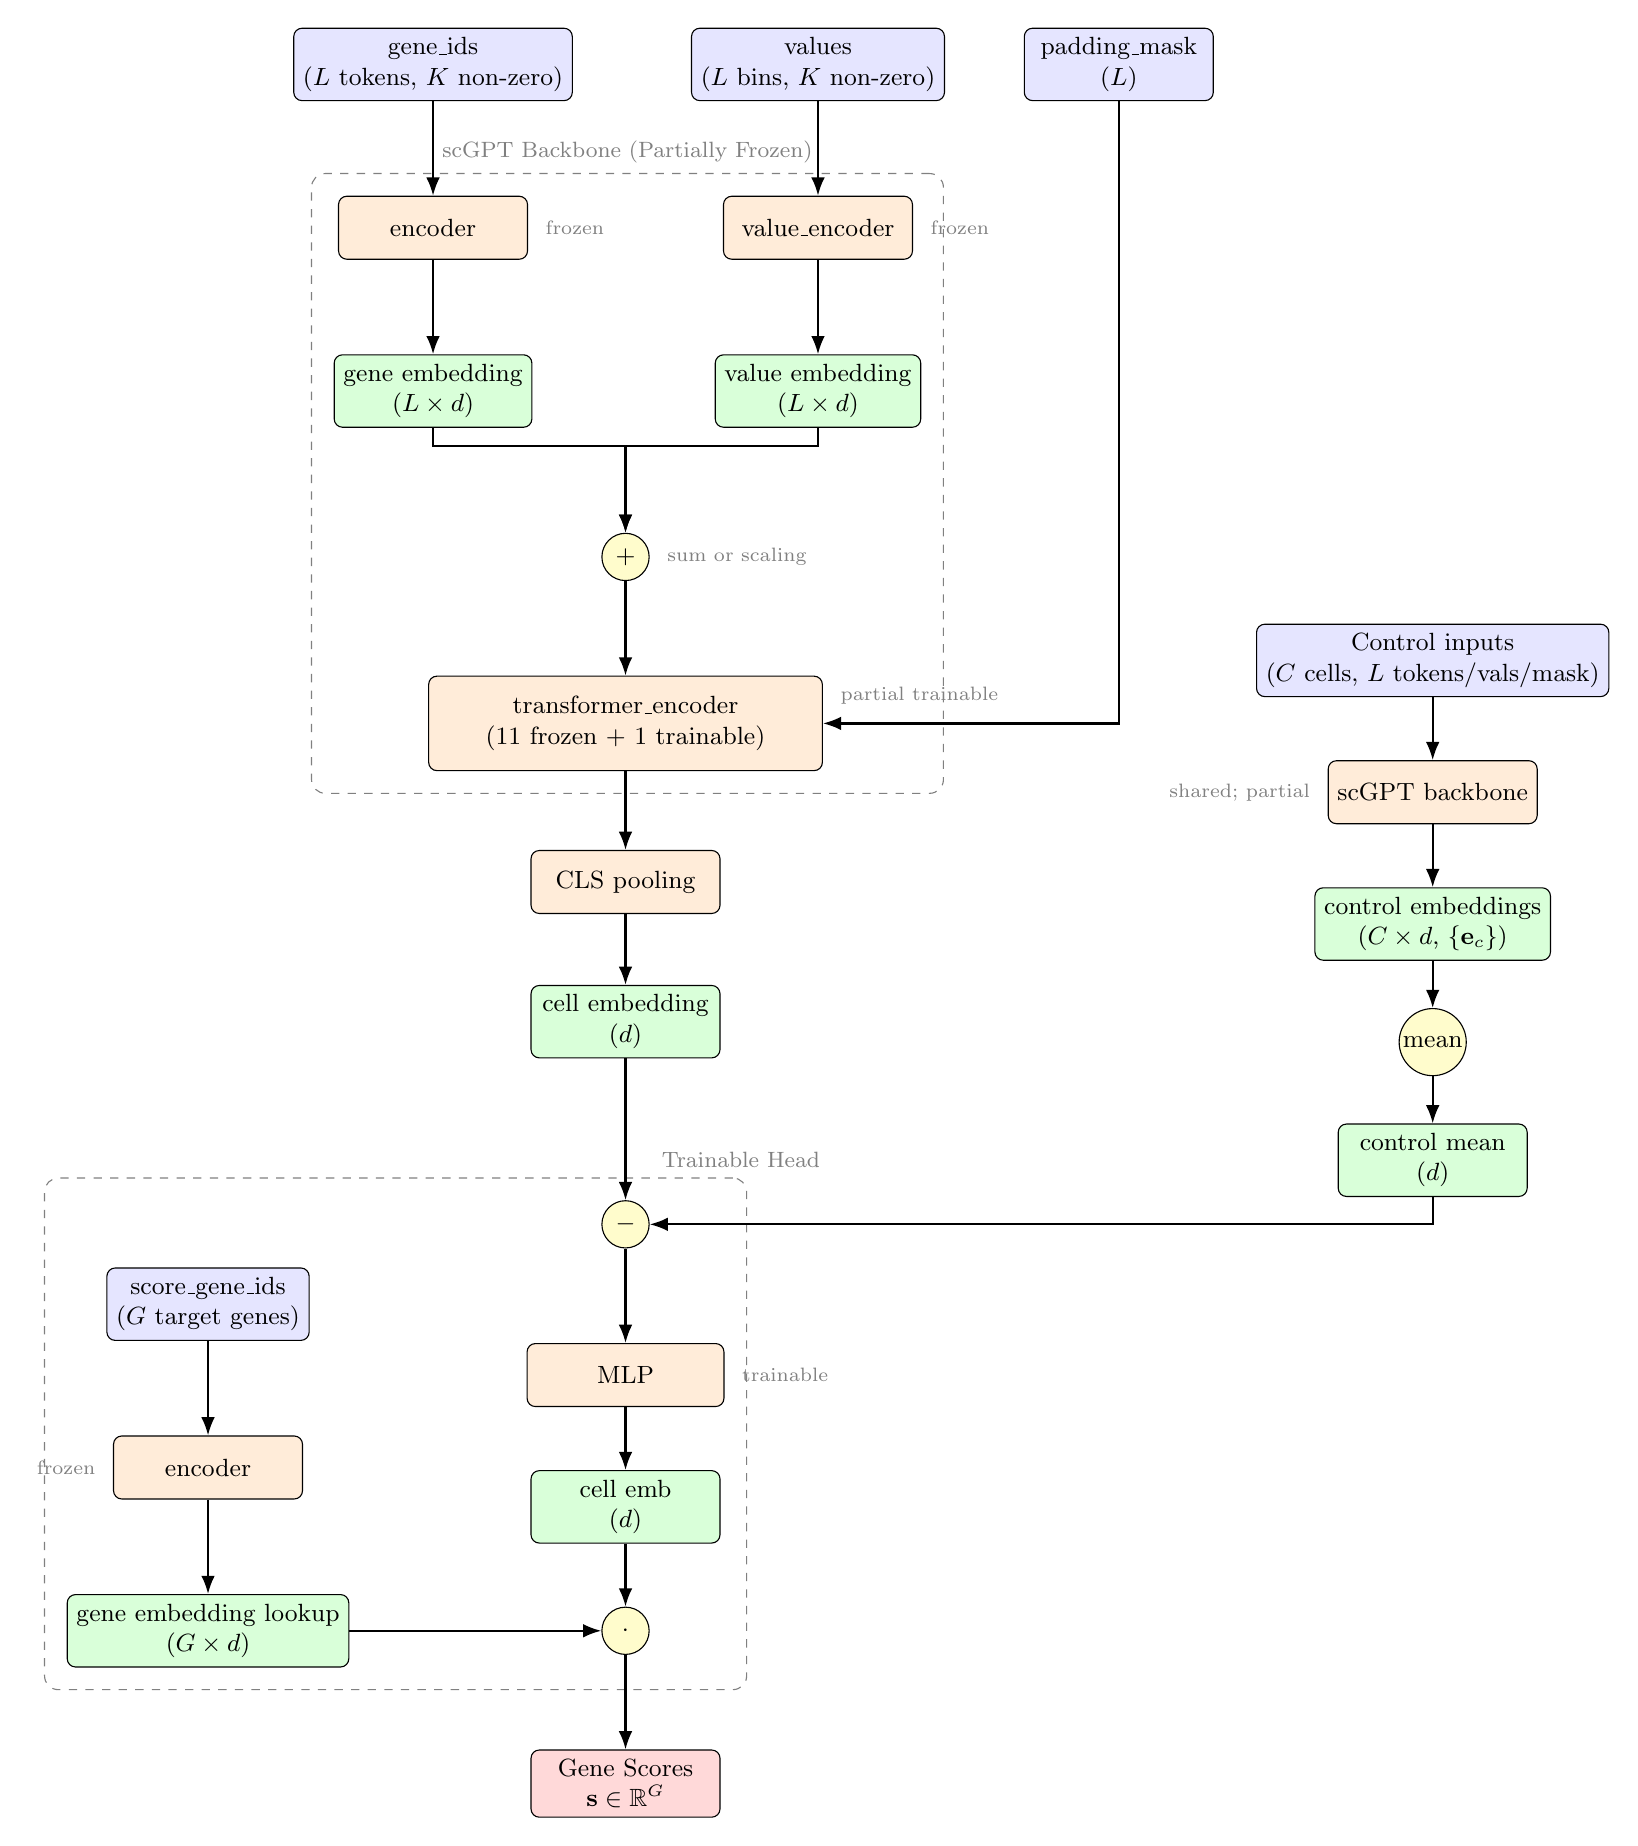
\begin{tikzpicture}[
    >=Latex,
    node distance=1.2cm and 2.4cm,
    font=\small,
    % Style definitions
    input/.style={draw, rounded corners=3pt, minimum width=2.4cm, minimum height=0.8cm, fill=blue!10, align=center},
    embed/.style={draw, rounded corners=3pt, minimum width=2.4cm, minimum height=0.8cm, fill=green!15, align=center},
    encoder/.style={draw, rounded corners=3pt, minimum width=2.4cm, minimum height=0.8cm, fill=orange!15, align=center},
    head/.style={draw, rounded corners=3pt, minimum width=2.4cm, minimum height=0.8cm, fill=yellow!15, align=center},
    unused/.style={draw, rounded corners=3pt, minimum width=2.4cm, minimum height=0.8cm, fill=gray!10, align=center, dashed},
    output/.style={draw, rounded corners=3pt, minimum width=2.4cm, minimum height=0.8cm, fill=red!15, align=center},
    operation/.style={circle, draw, minimum size=0.6cm, fill=yellow!20, inner sep=1pt},
    dashedbox/.style={draw, dashed, rounded corners=5pt, inner sep=8pt, gray},
    arrow/.style={->, thick, >=Latex, black},
]

%% ---------- INPUT LAYER ----------
\node[input] (gene_ids) {gene\_ids\\($L$ tokens, $K$ non-zero)};
\node[input, right=1.5cm of gene_ids] (values) {values\\($L$ bins, $K$ non-zero)};
\node[input, right=1cm of values] (padding) {padding\_mask\\($L$)};

%% ---------- ENCODERS + EMBEDDINGS (PARALLEL) ----------
\node[encoder, below=of gene_ids] (gene_encoder) {encoder};
\node[embed, below=of gene_encoder] (gene_emb) {gene embedding\\($L \times d$)};
\node[encoder, below=of values] (value_encoder) {value\_encoder};
\node[embed, below=of value_encoder] (value_emb) {value embedding\\($L \times d$)};

%% ---------- EMBEDDING FUSION ----------
\node[operation, below=1.8cm of $(gene_emb)!0.5!(value_emb)$] (add) {$+$};
\node[font=\scriptsize, gray, right=0.1cm of add.east] {sum or scaling};

%% ---------- TRANSFORMER ----------
\node[encoder, below=of add, minimum width=5cm, minimum height=1.2cm] (transformer) {transformer\_encoder\\(11 frozen + 1 trainable)};

%% ---------- OUTPUTS FROM TRANSFORMER ----------
\node[encoder, below=1.0cm of transformer] (cls_pool) {CLS pooling};
\node[embed, below=0.9cm of cls_pool] (cell_emb) {cell embedding\\($d$)};

%% ---------- CONTROL BRANCH ----------
\node[input, right=5.5cm of transformer, yshift=0.8cm] (control_branch) {Control inputs\\($C$ cells, $L$ tokens/vals/mask)};
\node[encoder, below=0.8cm of control_branch] (control_encoder) {scGPT backbone};
\node[embed, below=0.8cm of control_encoder] (control_emb) {control embeddings\\($C \times d$, $\{\mathbf{e}_c\}$)};
\node[operation, below=0.6cm of control_emb] (control_mean_op) {mean};
\node[embed, below=0.6cm of control_mean_op] (control_mean) {control mean\\($d$)};

%% ---------- DELTA EMBEDDING ----------
\node[operation, below=1.8cm of cell_emb] (subtract) {$-$};

%% ---------- GENE SCORING HEAD ----------
\node[encoder, below=of subtract, minimum width=2.5cm] (proj_mlp) {MLP};
\node[embed, below=0.8cm of proj_mlp] (cell_proj) {cell emb\\($d$)};
\node[operation, below=0.8cm of cell_proj] (dot_op) {$\cdot$};

%% ---------- OUTPUT ----------
\node[output, below=of dot_op] (scores) {Gene Scores\\$\mathbf{s} \in \mathbb{R}^{G}$};

%% ========== ARROWS ==========

% Inputs to encoders/embeddings
\draw[arrow] (gene_ids) -- (gene_encoder);
\draw[arrow] (gene_encoder) -- (gene_emb);
\draw[arrow] (values) -- (value_encoder);
\draw[arrow] (value_encoder) -- (value_emb);

% Embeddings to fusion (parallel)
\draw[arrow] (gene_emb) -- ++(0,-0.7) -| (add);
\draw[arrow] (value_emb) -- ++(0,-0.7) -| (add);

% Fusion to transformer
\draw[arrow] (add) -- (transformer);
\draw[arrow] (padding) |- (transformer);

% Transformer to cell embedding
\draw[arrow] (transformer.south) -- (cls_pool.north);
\draw[arrow] (cls_pool.south) -- (cell_emb.north);

% Control branch
\draw[arrow] (control_branch) -- (control_encoder);
\draw[arrow] (control_encoder) -- (control_emb);
\draw[arrow] (control_emb) -- (control_mean_op);
\draw[arrow] (control_mean_op) -- (control_mean);
\draw[arrow] (control_mean.south) |- (subtract.east);

% Cell embedding to delta
\draw[arrow] (cell_emb) -- (subtract);

% Delta to projection MLP
\draw[arrow] (subtract) -- (proj_mlp);
\draw[arrow] (proj_mlp) -- (cell_proj);
\draw[arrow] (cell_proj) -- (dot_op);

% Dot product to output
\draw[arrow] (dot_op) -- (scores);

% Gene embeddings to dot product (parallel flow)
\node[embed, left=3.2cm of dot_op] (gene_emb_lookup) {gene embedding lookup\\($G \times d$)};
\node[encoder, above=of gene_emb_lookup] (gene_emb_lookup_enc) {encoder};
\node[input, above=of gene_emb_lookup_enc] (score_gene_ids) {score\_gene\_ids\\($G$ target genes)};
\draw[arrow] (score_gene_ids) -- (gene_emb_lookup_enc);
\draw[arrow] (gene_emb_lookup_enc) -- (gene_emb_lookup);
\draw[arrow] (gene_emb_lookup.east) -- (dot_op.west);

%% ========== DASHED BOXES FOR GROUPING ==========

% scGPT Backbone box
\begin{scope}[on background layer]
    \node[dashedbox, fit=(gene_encoder)(value_encoder)(gene_emb)(value_emb)(add)(transformer), label={[font=\footnotesize, gray]above:scGPT Backbone (Partially Frozen)}] {};
\end{scope}

% Discriminative Head box
\begin{scope}[on background layer]
    \node[dashedbox, fit=(subtract)(proj_mlp)(cell_proj)(dot_op)(score_gene_ids)(gene_emb_lookup_enc)(gene_emb_lookup), label={[font=\footnotesize, gray]above right:Trainable Head}] {};
\end{scope}

%% ========== ANNOTATIONS ==========

% Trainability annotations
\node[font=\scriptsize, gray, right=0.1cm of gene_encoder.east] {frozen};
\node[font=\scriptsize, gray, right=0.1cm of value_encoder.east] {frozen};
\node[font=\scriptsize, gray, right=0.1cm of transformer.east, yshift=0.35cm] {partial trainable};
\node[font=\scriptsize, gray, left=0.1cm of control_encoder.west] {shared; partial};
\node[font=\scriptsize, gray, right=0.1cm of proj_mlp.east] {trainable};
\node[font=\scriptsize, gray, left=0.1cm of gene_emb_lookup_enc.west] {frozen};

\end{tikzpicture}
\ifexportfig
\else
\caption{Per-cell scGPT Discriminative Pipeline for Perturbation Gene Prediction.
For a single cell with $K$ non-zero genes, inputs are padded to length $L$.
Token IDs (\texttt{gene\_ids}), binned expression values, and a padding mask are fed to the scGPT backbone.
The \texttt{encoder} and \texttt{value\_encoder} produce gene/value embeddings, which are fused by element-wise addition (default)
or scaling (\texttt{input\_emb\_style}=\texttt{scaling}), then passed through \texttt{transformer\_encoder} to produce a CLS-based cell embedding.
A control branch runs the same backbone and the control mean is subtracted from the perturbed embedding.
The GeneScore head applies a projection MLP to the cell embedding before the dot product with the gene embedding lookup.
The \texttt{score\_gene\_ids} input is length $G$, the full set of candidate target genes, and its order defines the score output columns.
The backbone is partially frozen in this setup, with only the last transformer layer(s) and encoder norm optionally trainable.
Here, $G$ is the total number of genes in the dataset, $C$ is the number of control cells per perturbed cell, and $d$ is the embedding size.}
\label{fig:scgpt_pipeline}
\fi
\end{figure}

\end{document}
"
%   dvisvgm --libgs=/opt/homebrew/lib/libgs.dylib -o docs/report/final_report/scGPT_pipeline_standalone.svg docs/report/final_report/scGPT_pipeline_standalone_export.dvi
%   gs -sDEVICE=pngalpha -r300 -o docs/report/final_report/scGPT_pipeline_standalone.png docs/report/final_report/scGPT_pipeline_standalone_export.pdf

\documentclass{article}
\usepackage[margin=1cm]{geometry}
\usepackage{tikz}
\usepackage{amsmath,amssymb}
\usetikzlibrary{arrows.meta, positioning, shapes.geometric, calc, fit, backgrounds}
\newif\ifexportfig
\ifdefined\EXPORTFIG
\exportfigtrue
\else
\exportfigfalse
\fi

\begin{document}
\pagecolor{white}

\begin{figure}[htbp]
\centering
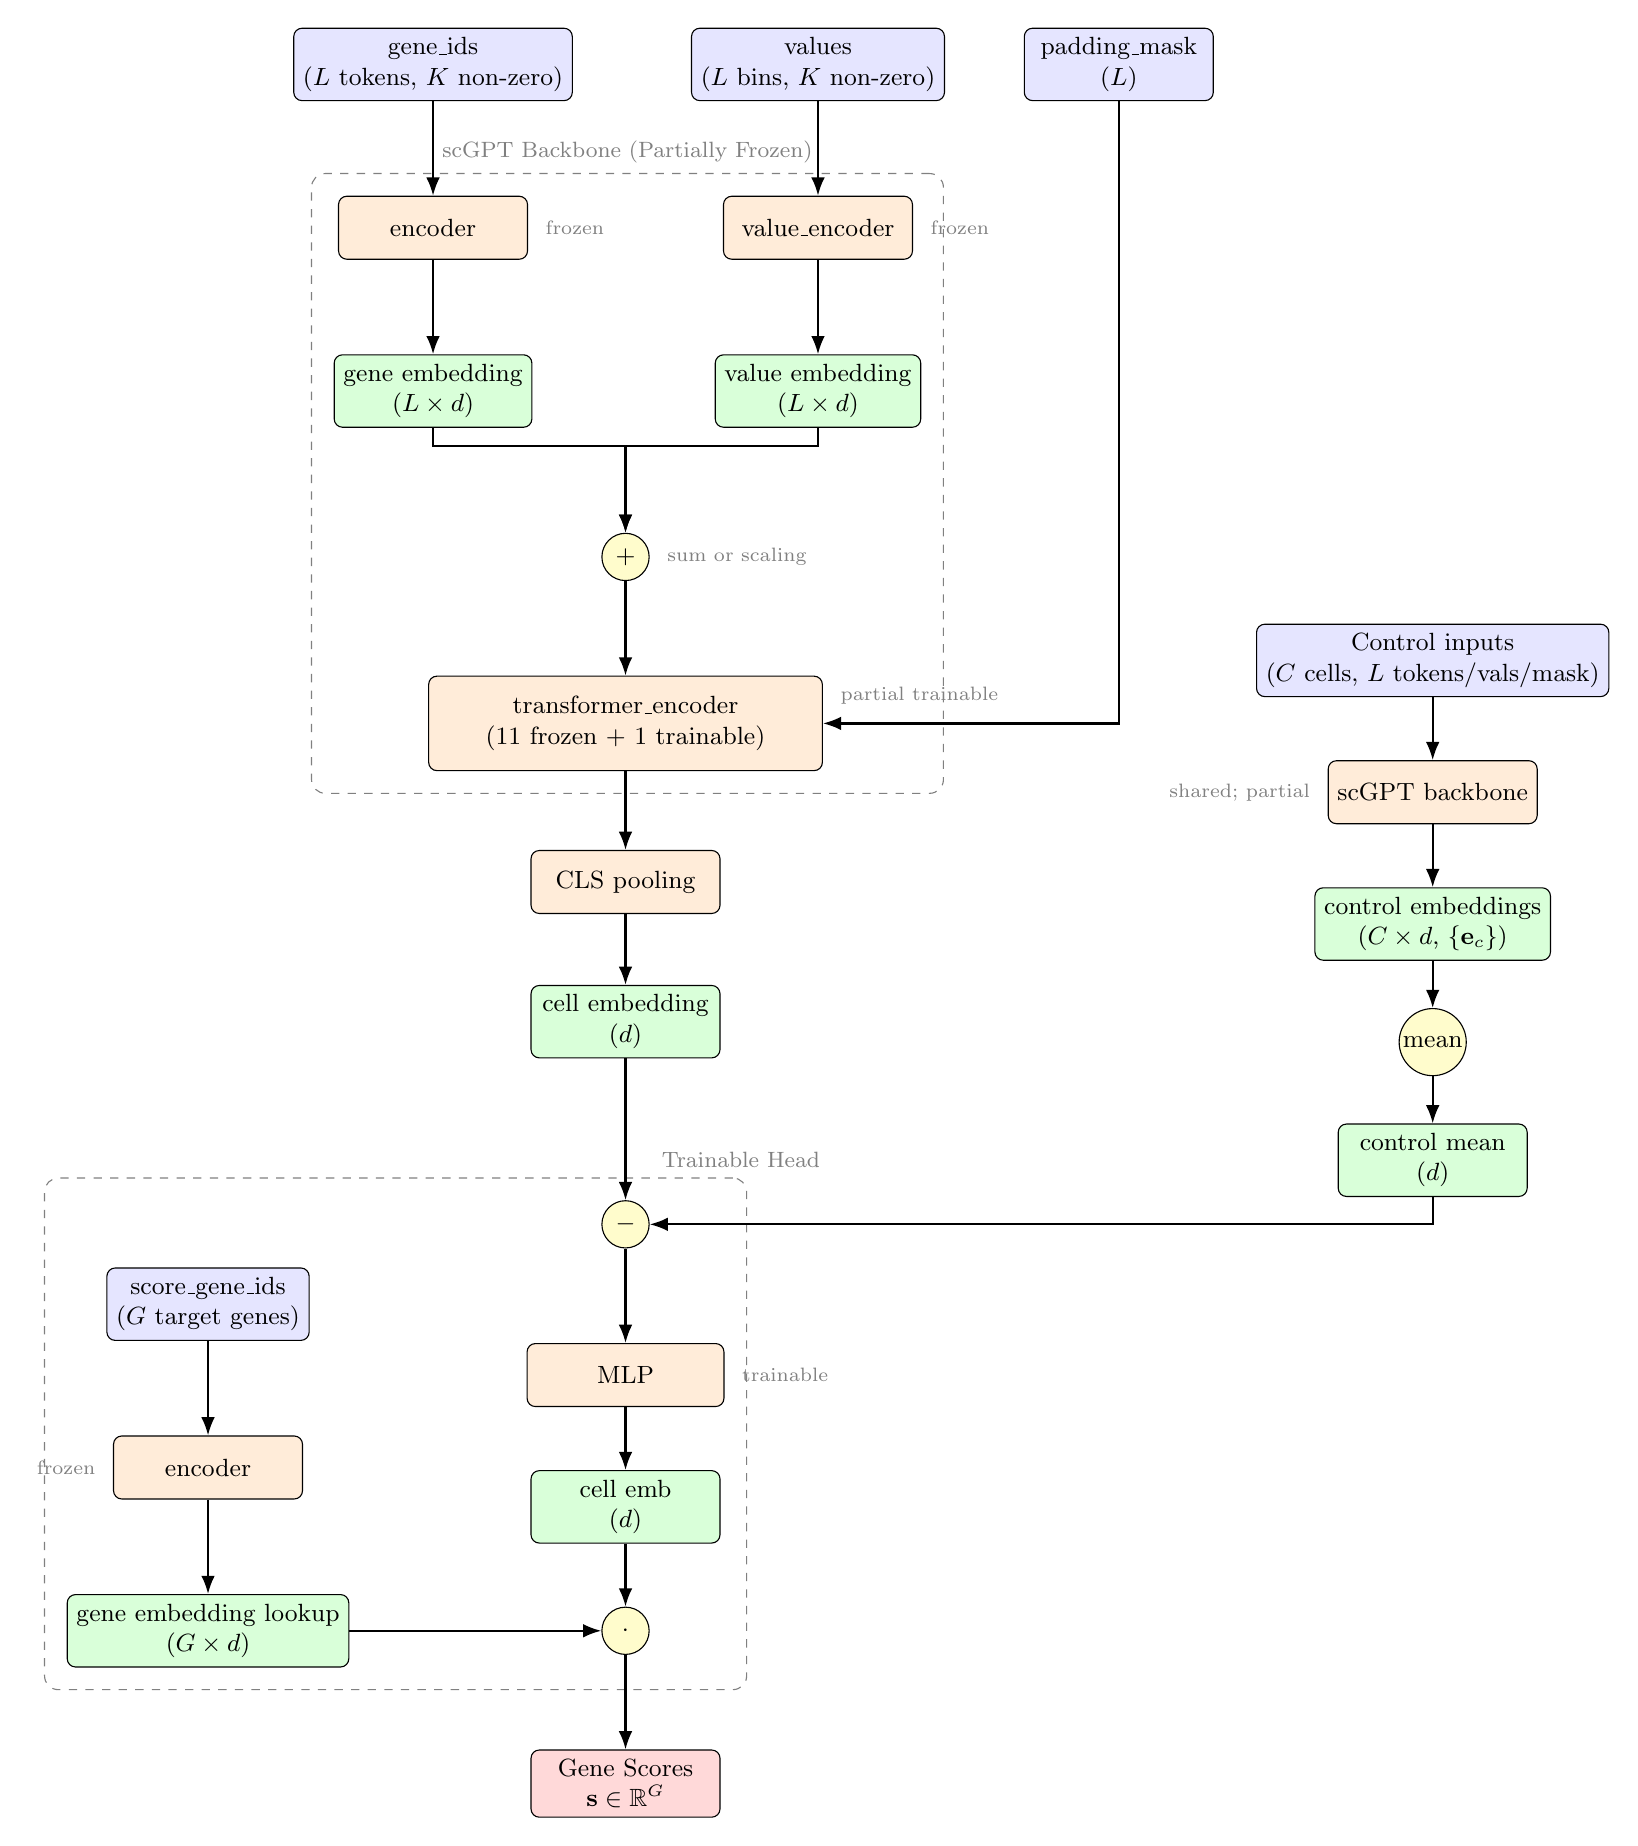
\begin{tikzpicture}[
    >=Latex,
    node distance=1.2cm and 2.4cm,
    font=\small,
    % Style definitions
    input/.style={draw, rounded corners=3pt, minimum width=2.4cm, minimum height=0.8cm, fill=blue!10, align=center},
    embed/.style={draw, rounded corners=3pt, minimum width=2.4cm, minimum height=0.8cm, fill=green!15, align=center},
    encoder/.style={draw, rounded corners=3pt, minimum width=2.4cm, minimum height=0.8cm, fill=orange!15, align=center},
    head/.style={draw, rounded corners=3pt, minimum width=2.4cm, minimum height=0.8cm, fill=yellow!15, align=center},
    unused/.style={draw, rounded corners=3pt, minimum width=2.4cm, minimum height=0.8cm, fill=gray!10, align=center, dashed},
    output/.style={draw, rounded corners=3pt, minimum width=2.4cm, minimum height=0.8cm, fill=red!15, align=center},
    operation/.style={circle, draw, minimum size=0.6cm, fill=yellow!20, inner sep=1pt},
    dashedbox/.style={draw, dashed, rounded corners=5pt, inner sep=8pt, gray},
    arrow/.style={->, thick, >=Latex, black},
]

%% ---------- INPUT LAYER ----------
\node[input] (gene_ids) {gene\_ids\\($L$ tokens, $K$ non-zero)};
\node[input, right=1.5cm of gene_ids] (values) {values\\($L$ bins, $K$ non-zero)};
\node[input, right=1cm of values] (padding) {padding\_mask\\($L$)};

%% ---------- ENCODERS + EMBEDDINGS (PARALLEL) ----------
\node[encoder, below=of gene_ids] (gene_encoder) {encoder};
\node[embed, below=of gene_encoder] (gene_emb) {gene embedding\\($L \times d$)};
\node[encoder, below=of values] (value_encoder) {value\_encoder};
\node[embed, below=of value_encoder] (value_emb) {value embedding\\($L \times d$)};

%% ---------- EMBEDDING FUSION ----------
\node[operation, below=1.8cm of $(gene_emb)!0.5!(value_emb)$] (add) {$+$};
\node[font=\scriptsize, gray, right=0.1cm of add.east] {sum or scaling};

%% ---------- TRANSFORMER ----------
\node[encoder, below=of add, minimum width=5cm, minimum height=1.2cm] (transformer) {transformer\_encoder\\(11 frozen + 1 trainable)};

%% ---------- OUTPUTS FROM TRANSFORMER ----------
\node[encoder, below=1.0cm of transformer] (cls_pool) {CLS pooling};
\node[embed, below=0.9cm of cls_pool] (cell_emb) {cell embedding\\($d$)};

%% ---------- CONTROL BRANCH ----------
\node[input, right=5.5cm of transformer, yshift=0.8cm] (control_branch) {Control inputs\\($C$ cells, $L$ tokens/vals/mask)};
\node[encoder, below=0.8cm of control_branch] (control_encoder) {scGPT backbone};
\node[embed, below=0.8cm of control_encoder] (control_emb) {control embeddings\\($C \times d$, $\{\mathbf{e}_c\}$)};
\node[operation, below=0.6cm of control_emb] (control_mean_op) {mean};
\node[embed, below=0.6cm of control_mean_op] (control_mean) {control mean\\($d$)};

%% ---------- DELTA EMBEDDING ----------
\node[operation, below=1.8cm of cell_emb] (subtract) {$-$};

%% ---------- GENE SCORING HEAD ----------
\node[encoder, below=of subtract, minimum width=2.5cm] (proj_mlp) {MLP};
\node[embed, below=0.8cm of proj_mlp] (cell_proj) {cell emb\\($d$)};
\node[operation, below=0.8cm of cell_proj] (dot_op) {$\cdot$};

%% ---------- OUTPUT ----------
\node[output, below=of dot_op] (scores) {Gene Scores\\$\mathbf{s} \in \mathbb{R}^{G}$};

%% ========== ARROWS ==========

% Inputs to encoders/embeddings
\draw[arrow] (gene_ids) -- (gene_encoder);
\draw[arrow] (gene_encoder) -- (gene_emb);
\draw[arrow] (values) -- (value_encoder);
\draw[arrow] (value_encoder) -- (value_emb);

% Embeddings to fusion (parallel)
\draw[arrow] (gene_emb) -- ++(0,-0.7) -| (add);
\draw[arrow] (value_emb) -- ++(0,-0.7) -| (add);

% Fusion to transformer
\draw[arrow] (add) -- (transformer);
\draw[arrow] (padding) |- (transformer);

% Transformer to cell embedding
\draw[arrow] (transformer.south) -- (cls_pool.north);
\draw[arrow] (cls_pool.south) -- (cell_emb.north);

% Control branch
\draw[arrow] (control_branch) -- (control_encoder);
\draw[arrow] (control_encoder) -- (control_emb);
\draw[arrow] (control_emb) -- (control_mean_op);
\draw[arrow] (control_mean_op) -- (control_mean);
\draw[arrow] (control_mean.south) |- (subtract.east);

% Cell embedding to delta
\draw[arrow] (cell_emb) -- (subtract);

% Delta to projection MLP
\draw[arrow] (subtract) -- (proj_mlp);
\draw[arrow] (proj_mlp) -- (cell_proj);
\draw[arrow] (cell_proj) -- (dot_op);

% Dot product to output
\draw[arrow] (dot_op) -- (scores);

% Gene embeddings to dot product (parallel flow)
\node[embed, left=3.2cm of dot_op] (gene_emb_lookup) {gene embedding lookup\\($G \times d$)};
\node[encoder, above=of gene_emb_lookup] (gene_emb_lookup_enc) {encoder};
\node[input, above=of gene_emb_lookup_enc] (score_gene_ids) {score\_gene\_ids\\($G$ target genes)};
\draw[arrow] (score_gene_ids) -- (gene_emb_lookup_enc);
\draw[arrow] (gene_emb_lookup_enc) -- (gene_emb_lookup);
\draw[arrow] (gene_emb_lookup.east) -- (dot_op.west);

%% ========== DASHED BOXES FOR GROUPING ==========

% scGPT Backbone box
\begin{scope}[on background layer]
    \node[dashedbox, fit=(gene_encoder)(value_encoder)(gene_emb)(value_emb)(add)(transformer), label={[font=\footnotesize, gray]above:scGPT Backbone (Partially Frozen)}] {};
\end{scope}

% Discriminative Head box
\begin{scope}[on background layer]
    \node[dashedbox, fit=(subtract)(proj_mlp)(cell_proj)(dot_op)(score_gene_ids)(gene_emb_lookup_enc)(gene_emb_lookup), label={[font=\footnotesize, gray]above right:Trainable Head}] {};
\end{scope}

%% ========== ANNOTATIONS ==========

% Trainability annotations
\node[font=\scriptsize, gray, right=0.1cm of gene_encoder.east] {frozen};
\node[font=\scriptsize, gray, right=0.1cm of value_encoder.east] {frozen};
\node[font=\scriptsize, gray, right=0.1cm of transformer.east, yshift=0.35cm] {partial trainable};
\node[font=\scriptsize, gray, left=0.1cm of control_encoder.west] {shared; partial};
\node[font=\scriptsize, gray, right=0.1cm of proj_mlp.east] {trainable};
\node[font=\scriptsize, gray, left=0.1cm of gene_emb_lookup_enc.west] {frozen};

\end{tikzpicture}
\ifexportfig
\else
\caption{Per-cell scGPT Discriminative Pipeline for Perturbation Gene Prediction.
For a single cell with $K$ non-zero genes, inputs are padded to length $L$.
Token IDs (\texttt{gene\_ids}), binned expression values, and a padding mask are fed to the scGPT backbone.
The \texttt{encoder} and \texttt{value\_encoder} produce gene/value embeddings, which are fused by element-wise addition (default)
or scaling (\texttt{input\_emb\_style}=\texttt{scaling}), then passed through \texttt{transformer\_encoder} to produce a CLS-based cell embedding.
A control branch runs the same backbone and the control mean is subtracted from the perturbed embedding.
The GeneScore head applies a projection MLP to the cell embedding before the dot product with the gene embedding lookup.
The \texttt{score\_gene\_ids} input is length $G$, the full set of candidate target genes, and its order defines the score output columns.
The backbone is partially frozen in this setup, with only the last transformer layer(s) and encoder norm optionally trainable.
Here, $G$ is the total number of genes in the dataset, $C$ is the number of control cells per perturbed cell, and $d$ is the embedding size.}
\label{fig:scgpt_pipeline}
\fi
\end{figure}

\end{document}
"
%   latex -interaction=nonstopmode -halt-on-error -jobname scGPT_pipeline_standalone_export -output-directory docs/report/final_report "\\def\\EXPORTFIG{1}\% scGPT Discriminative Pipeline Architecture (Standalone)
% Export (caption-free) SVG/PNG:
%   pdflatex -interaction=nonstopmode -halt-on-error -jobname scGPT_pipeline_standalone_export -output-directory docs/report/final_report "\\def\\EXPORTFIG{1}\% scGPT Discriminative Pipeline Architecture (Standalone)
% Export (caption-free) SVG/PNG:
%   pdflatex -interaction=nonstopmode -halt-on-error -jobname scGPT_pipeline_standalone_export -output-directory docs/report/final_report "\\def\\EXPORTFIG{1}\\input{docs/report/final_report/scGPT_pipeline_standalone.tex}"
%   latex -interaction=nonstopmode -halt-on-error -jobname scGPT_pipeline_standalone_export -output-directory docs/report/final_report "\\def\\EXPORTFIG{1}\\input{docs/report/final_report/scGPT_pipeline_standalone.tex}"
%   dvisvgm --libgs=/opt/homebrew/lib/libgs.dylib -o docs/report/final_report/scGPT_pipeline_standalone.svg docs/report/final_report/scGPT_pipeline_standalone_export.dvi
%   gs -sDEVICE=pngalpha -r300 -o docs/report/final_report/scGPT_pipeline_standalone.png docs/report/final_report/scGPT_pipeline_standalone_export.pdf

\documentclass{article}
\usepackage[margin=1cm]{geometry}
\usepackage{tikz}
\usepackage{amsmath,amssymb}
\usetikzlibrary{arrows.meta, positioning, shapes.geometric, calc, fit, backgrounds}
\newif\ifexportfig
\ifdefined\EXPORTFIG
\exportfigtrue
\else
\exportfigfalse
\fi

\begin{document}
\pagecolor{white}

\begin{figure}[htbp]
\centering
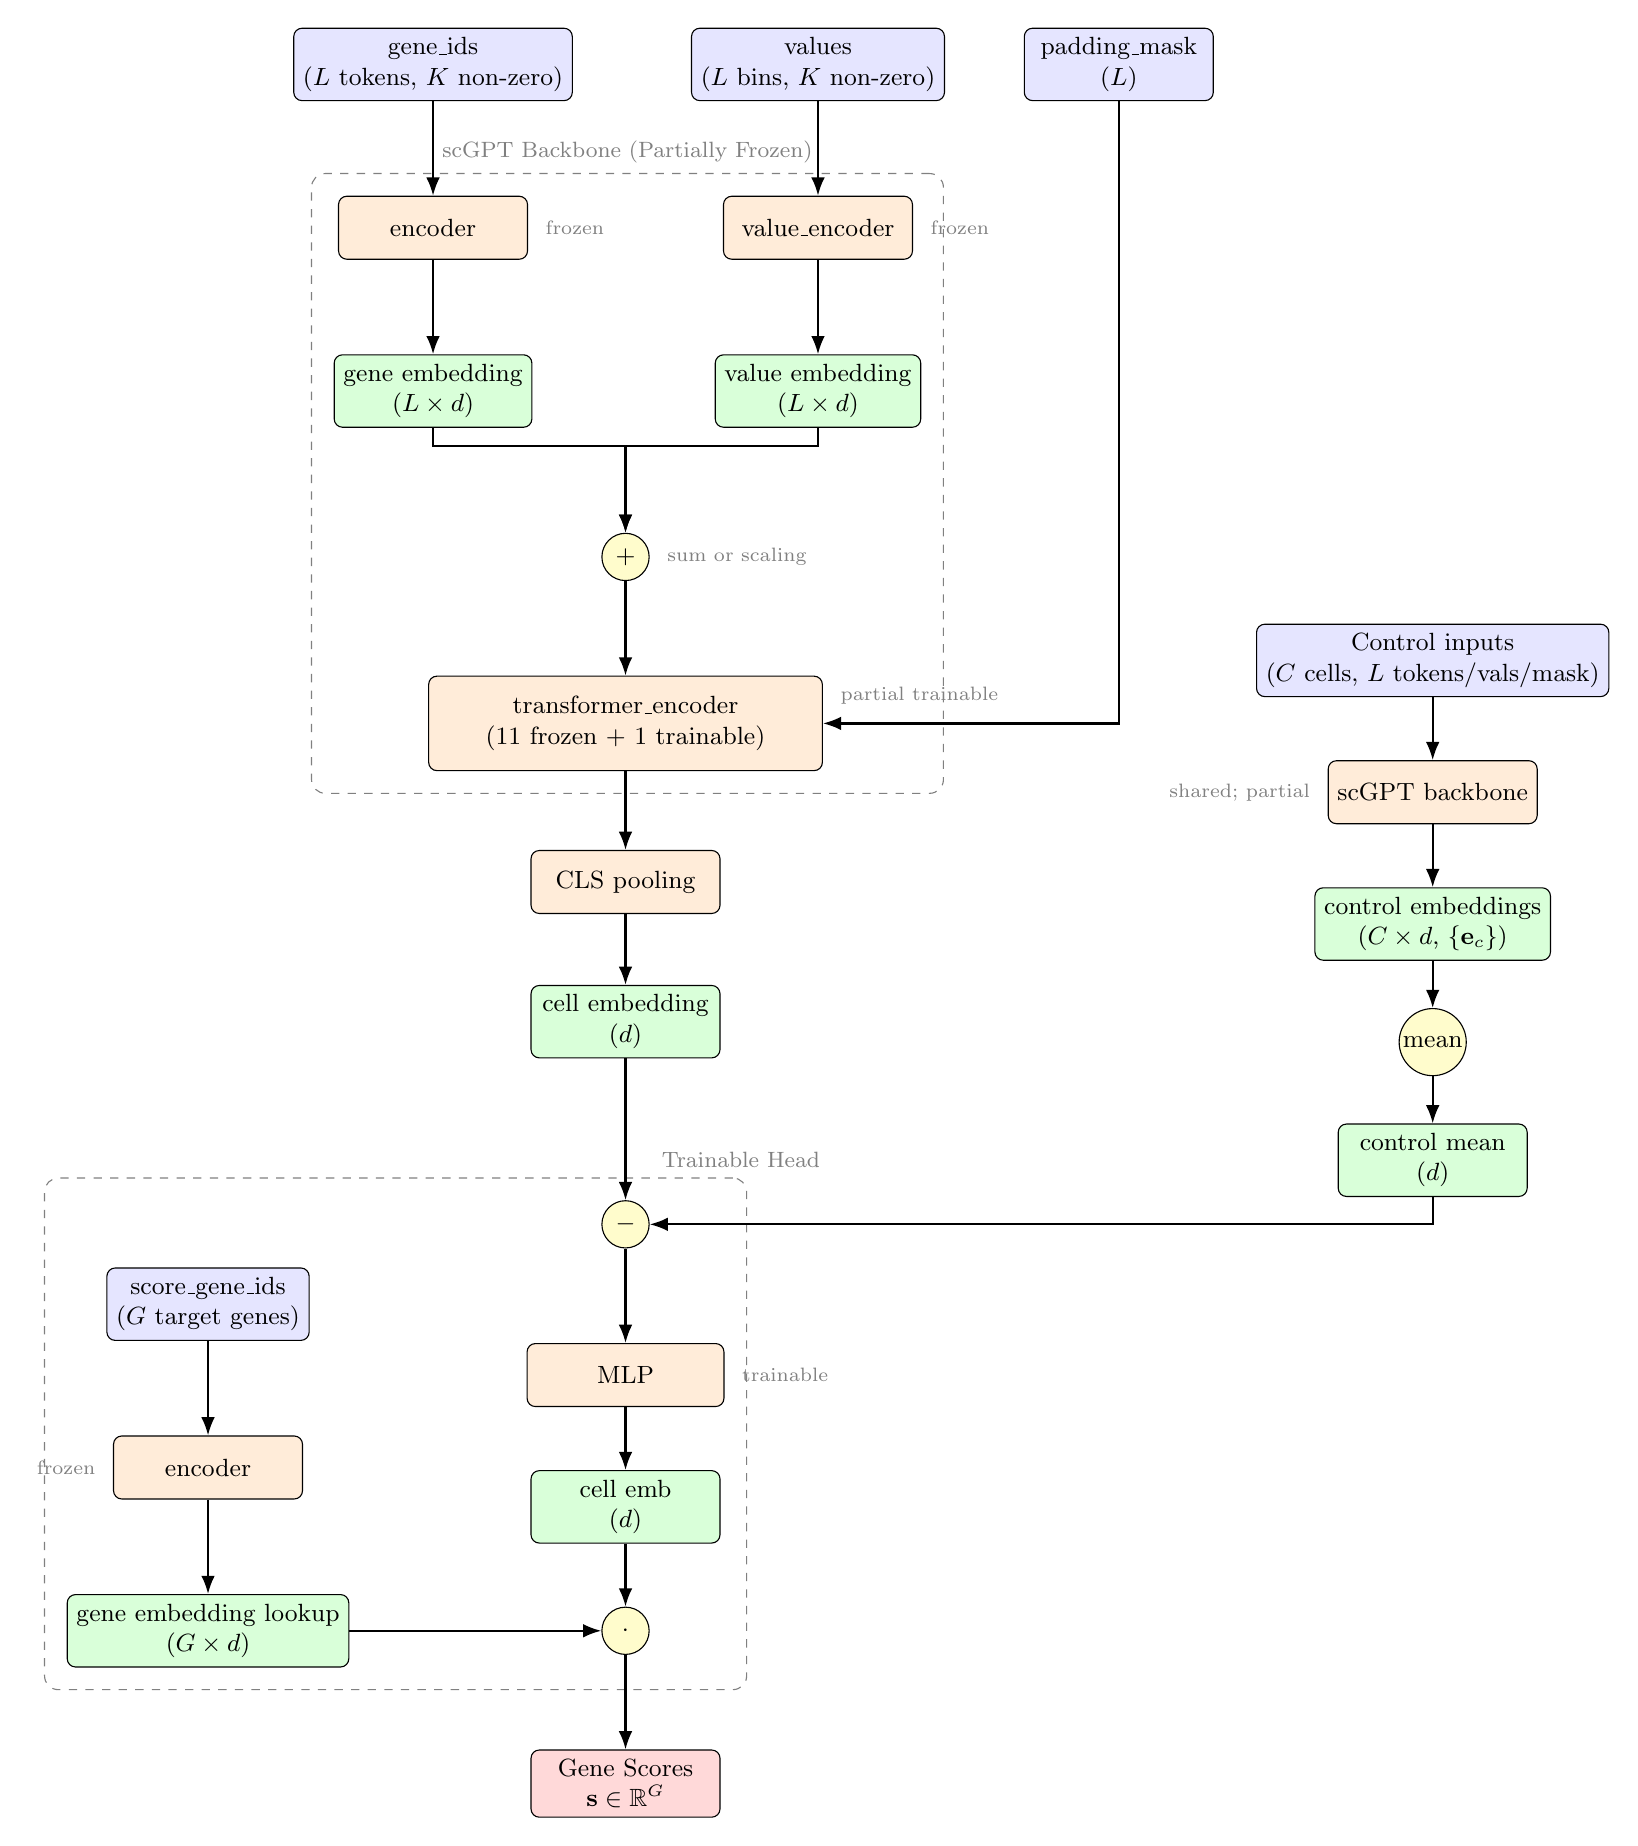
\begin{tikzpicture}[
    >=Latex,
    node distance=1.2cm and 2.4cm,
    font=\small,
    % Style definitions
    input/.style={draw, rounded corners=3pt, minimum width=2.4cm, minimum height=0.8cm, fill=blue!10, align=center},
    embed/.style={draw, rounded corners=3pt, minimum width=2.4cm, minimum height=0.8cm, fill=green!15, align=center},
    encoder/.style={draw, rounded corners=3pt, minimum width=2.4cm, minimum height=0.8cm, fill=orange!15, align=center},
    head/.style={draw, rounded corners=3pt, minimum width=2.4cm, minimum height=0.8cm, fill=yellow!15, align=center},
    unused/.style={draw, rounded corners=3pt, minimum width=2.4cm, minimum height=0.8cm, fill=gray!10, align=center, dashed},
    output/.style={draw, rounded corners=3pt, minimum width=2.4cm, minimum height=0.8cm, fill=red!15, align=center},
    operation/.style={circle, draw, minimum size=0.6cm, fill=yellow!20, inner sep=1pt},
    dashedbox/.style={draw, dashed, rounded corners=5pt, inner sep=8pt, gray},
    arrow/.style={->, thick, >=Latex, black},
]

%% ---------- INPUT LAYER ----------
\node[input] (gene_ids) {gene\_ids\\($L$ tokens, $K$ non-zero)};
\node[input, right=1.5cm of gene_ids] (values) {values\\($L$ bins, $K$ non-zero)};
\node[input, right=1cm of values] (padding) {padding\_mask\\($L$)};

%% ---------- ENCODERS + EMBEDDINGS (PARALLEL) ----------
\node[encoder, below=of gene_ids] (gene_encoder) {encoder};
\node[embed, below=of gene_encoder] (gene_emb) {gene embedding\\($L \times d$)};
\node[encoder, below=of values] (value_encoder) {value\_encoder};
\node[embed, below=of value_encoder] (value_emb) {value embedding\\($L \times d$)};

%% ---------- EMBEDDING FUSION ----------
\node[operation, below=1.8cm of $(gene_emb)!0.5!(value_emb)$] (add) {$+$};
\node[font=\scriptsize, gray, right=0.1cm of add.east] {sum or scaling};

%% ---------- TRANSFORMER ----------
\node[encoder, below=of add, minimum width=5cm, minimum height=1.2cm] (transformer) {transformer\_encoder\\(11 frozen + 1 trainable)};

%% ---------- OUTPUTS FROM TRANSFORMER ----------
\node[encoder, below=1.0cm of transformer] (cls_pool) {CLS pooling};
\node[embed, below=0.9cm of cls_pool] (cell_emb) {cell embedding\\($d$)};

%% ---------- CONTROL BRANCH ----------
\node[input, right=5.5cm of transformer, yshift=0.8cm] (control_branch) {Control inputs\\($C$ cells, $L$ tokens/vals/mask)};
\node[encoder, below=0.8cm of control_branch] (control_encoder) {scGPT backbone};
\node[embed, below=0.8cm of control_encoder] (control_emb) {control embeddings\\($C \times d$, $\{\mathbf{e}_c\}$)};
\node[operation, below=0.6cm of control_emb] (control_mean_op) {mean};
\node[embed, below=0.6cm of control_mean_op] (control_mean) {control mean\\($d$)};

%% ---------- DELTA EMBEDDING ----------
\node[operation, below=1.8cm of cell_emb] (subtract) {$-$};

%% ---------- GENE SCORING HEAD ----------
\node[encoder, below=of subtract, minimum width=2.5cm] (proj_mlp) {MLP};
\node[embed, below=0.8cm of proj_mlp] (cell_proj) {cell emb\\($d$)};
\node[operation, below=0.8cm of cell_proj] (dot_op) {$\cdot$};

%% ---------- OUTPUT ----------
\node[output, below=of dot_op] (scores) {Gene Scores\\$\mathbf{s} \in \mathbb{R}^{G}$};

%% ========== ARROWS ==========

% Inputs to encoders/embeddings
\draw[arrow] (gene_ids) -- (gene_encoder);
\draw[arrow] (gene_encoder) -- (gene_emb);
\draw[arrow] (values) -- (value_encoder);
\draw[arrow] (value_encoder) -- (value_emb);

% Embeddings to fusion (parallel)
\draw[arrow] (gene_emb) -- ++(0,-0.7) -| (add);
\draw[arrow] (value_emb) -- ++(0,-0.7) -| (add);

% Fusion to transformer
\draw[arrow] (add) -- (transformer);
\draw[arrow] (padding) |- (transformer);

% Transformer to cell embedding
\draw[arrow] (transformer.south) -- (cls_pool.north);
\draw[arrow] (cls_pool.south) -- (cell_emb.north);

% Control branch
\draw[arrow] (control_branch) -- (control_encoder);
\draw[arrow] (control_encoder) -- (control_emb);
\draw[arrow] (control_emb) -- (control_mean_op);
\draw[arrow] (control_mean_op) -- (control_mean);
\draw[arrow] (control_mean.south) |- (subtract.east);

% Cell embedding to delta
\draw[arrow] (cell_emb) -- (subtract);

% Delta to projection MLP
\draw[arrow] (subtract) -- (proj_mlp);
\draw[arrow] (proj_mlp) -- (cell_proj);
\draw[arrow] (cell_proj) -- (dot_op);

% Dot product to output
\draw[arrow] (dot_op) -- (scores);

% Gene embeddings to dot product (parallel flow)
\node[embed, left=3.2cm of dot_op] (gene_emb_lookup) {gene embedding lookup\\($G \times d$)};
\node[encoder, above=of gene_emb_lookup] (gene_emb_lookup_enc) {encoder};
\node[input, above=of gene_emb_lookup_enc] (score_gene_ids) {score\_gene\_ids\\($G$ target genes)};
\draw[arrow] (score_gene_ids) -- (gene_emb_lookup_enc);
\draw[arrow] (gene_emb_lookup_enc) -- (gene_emb_lookup);
\draw[arrow] (gene_emb_lookup.east) -- (dot_op.west);

%% ========== DASHED BOXES FOR GROUPING ==========

% scGPT Backbone box
\begin{scope}[on background layer]
    \node[dashedbox, fit=(gene_encoder)(value_encoder)(gene_emb)(value_emb)(add)(transformer), label={[font=\footnotesize, gray]above:scGPT Backbone (Partially Frozen)}] {};
\end{scope}

% Discriminative Head box
\begin{scope}[on background layer]
    \node[dashedbox, fit=(subtract)(proj_mlp)(cell_proj)(dot_op)(score_gene_ids)(gene_emb_lookup_enc)(gene_emb_lookup), label={[font=\footnotesize, gray]above right:Trainable Head}] {};
\end{scope}

%% ========== ANNOTATIONS ==========

% Trainability annotations
\node[font=\scriptsize, gray, right=0.1cm of gene_encoder.east] {frozen};
\node[font=\scriptsize, gray, right=0.1cm of value_encoder.east] {frozen};
\node[font=\scriptsize, gray, right=0.1cm of transformer.east, yshift=0.35cm] {partial trainable};
\node[font=\scriptsize, gray, left=0.1cm of control_encoder.west] {shared; partial};
\node[font=\scriptsize, gray, right=0.1cm of proj_mlp.east] {trainable};
\node[font=\scriptsize, gray, left=0.1cm of gene_emb_lookup_enc.west] {frozen};

\end{tikzpicture}
\ifexportfig
\else
\caption{Per-cell scGPT Discriminative Pipeline for Perturbation Gene Prediction.
For a single cell with $K$ non-zero genes, inputs are padded to length $L$.
Token IDs (\texttt{gene\_ids}), binned expression values, and a padding mask are fed to the scGPT backbone.
The \texttt{encoder} and \texttt{value\_encoder} produce gene/value embeddings, which are fused by element-wise addition (default)
or scaling (\texttt{input\_emb\_style}=\texttt{scaling}), then passed through \texttt{transformer\_encoder} to produce a CLS-based cell embedding.
A control branch runs the same backbone and the control mean is subtracted from the perturbed embedding.
The GeneScore head applies a projection MLP to the cell embedding before the dot product with the gene embedding lookup.
The \texttt{score\_gene\_ids} input is length $G$, the full set of candidate target genes, and its order defines the score output columns.
The backbone is partially frozen in this setup, with only the last transformer layer(s) and encoder norm optionally trainable.
Here, $G$ is the total number of genes in the dataset, $C$ is the number of control cells per perturbed cell, and $d$ is the embedding size.}
\label{fig:scgpt_pipeline}
\fi
\end{figure}

\end{document}
"
%   latex -interaction=nonstopmode -halt-on-error -jobname scGPT_pipeline_standalone_export -output-directory docs/report/final_report "\\def\\EXPORTFIG{1}\% scGPT Discriminative Pipeline Architecture (Standalone)
% Export (caption-free) SVG/PNG:
%   pdflatex -interaction=nonstopmode -halt-on-error -jobname scGPT_pipeline_standalone_export -output-directory docs/report/final_report "\\def\\EXPORTFIG{1}\\input{docs/report/final_report/scGPT_pipeline_standalone.tex}"
%   latex -interaction=nonstopmode -halt-on-error -jobname scGPT_pipeline_standalone_export -output-directory docs/report/final_report "\\def\\EXPORTFIG{1}\\input{docs/report/final_report/scGPT_pipeline_standalone.tex}"
%   dvisvgm --libgs=/opt/homebrew/lib/libgs.dylib -o docs/report/final_report/scGPT_pipeline_standalone.svg docs/report/final_report/scGPT_pipeline_standalone_export.dvi
%   gs -sDEVICE=pngalpha -r300 -o docs/report/final_report/scGPT_pipeline_standalone.png docs/report/final_report/scGPT_pipeline_standalone_export.pdf

\documentclass{article}
\usepackage[margin=1cm]{geometry}
\usepackage{tikz}
\usepackage{amsmath,amssymb}
\usetikzlibrary{arrows.meta, positioning, shapes.geometric, calc, fit, backgrounds}
\newif\ifexportfig
\ifdefined\EXPORTFIG
\exportfigtrue
\else
\exportfigfalse
\fi

\begin{document}
\pagecolor{white}

\begin{figure}[htbp]
\centering
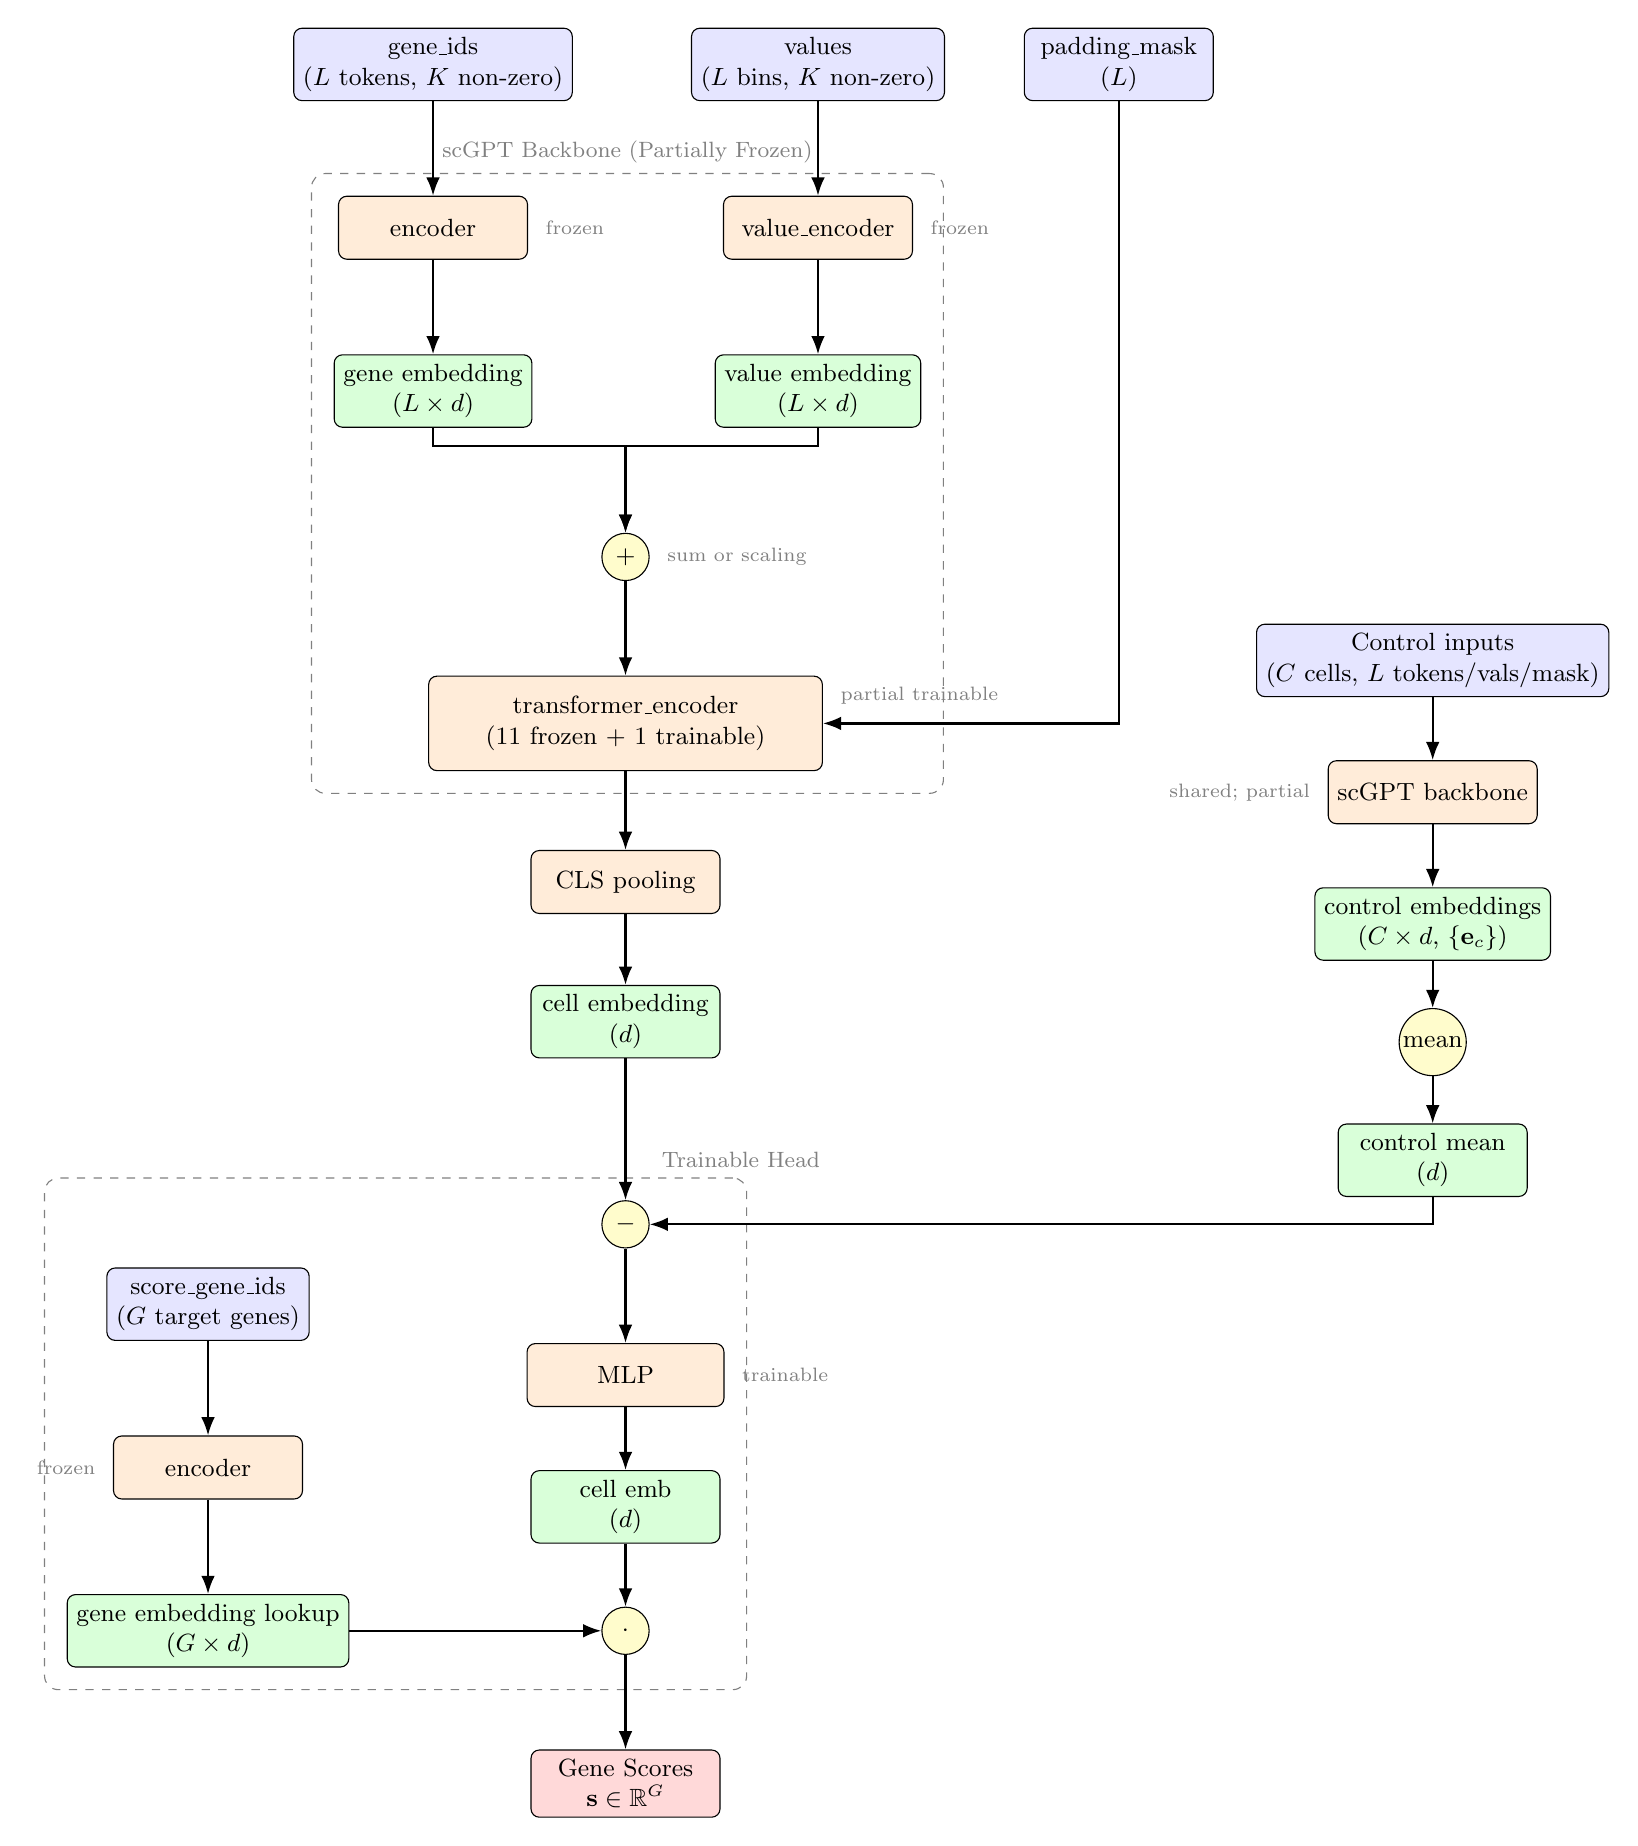
\begin{tikzpicture}[
    >=Latex,
    node distance=1.2cm and 2.4cm,
    font=\small,
    % Style definitions
    input/.style={draw, rounded corners=3pt, minimum width=2.4cm, minimum height=0.8cm, fill=blue!10, align=center},
    embed/.style={draw, rounded corners=3pt, minimum width=2.4cm, minimum height=0.8cm, fill=green!15, align=center},
    encoder/.style={draw, rounded corners=3pt, minimum width=2.4cm, minimum height=0.8cm, fill=orange!15, align=center},
    head/.style={draw, rounded corners=3pt, minimum width=2.4cm, minimum height=0.8cm, fill=yellow!15, align=center},
    unused/.style={draw, rounded corners=3pt, minimum width=2.4cm, minimum height=0.8cm, fill=gray!10, align=center, dashed},
    output/.style={draw, rounded corners=3pt, minimum width=2.4cm, minimum height=0.8cm, fill=red!15, align=center},
    operation/.style={circle, draw, minimum size=0.6cm, fill=yellow!20, inner sep=1pt},
    dashedbox/.style={draw, dashed, rounded corners=5pt, inner sep=8pt, gray},
    arrow/.style={->, thick, >=Latex, black},
]

%% ---------- INPUT LAYER ----------
\node[input] (gene_ids) {gene\_ids\\($L$ tokens, $K$ non-zero)};
\node[input, right=1.5cm of gene_ids] (values) {values\\($L$ bins, $K$ non-zero)};
\node[input, right=1cm of values] (padding) {padding\_mask\\($L$)};

%% ---------- ENCODERS + EMBEDDINGS (PARALLEL) ----------
\node[encoder, below=of gene_ids] (gene_encoder) {encoder};
\node[embed, below=of gene_encoder] (gene_emb) {gene embedding\\($L \times d$)};
\node[encoder, below=of values] (value_encoder) {value\_encoder};
\node[embed, below=of value_encoder] (value_emb) {value embedding\\($L \times d$)};

%% ---------- EMBEDDING FUSION ----------
\node[operation, below=1.8cm of $(gene_emb)!0.5!(value_emb)$] (add) {$+$};
\node[font=\scriptsize, gray, right=0.1cm of add.east] {sum or scaling};

%% ---------- TRANSFORMER ----------
\node[encoder, below=of add, minimum width=5cm, minimum height=1.2cm] (transformer) {transformer\_encoder\\(11 frozen + 1 trainable)};

%% ---------- OUTPUTS FROM TRANSFORMER ----------
\node[encoder, below=1.0cm of transformer] (cls_pool) {CLS pooling};
\node[embed, below=0.9cm of cls_pool] (cell_emb) {cell embedding\\($d$)};

%% ---------- CONTROL BRANCH ----------
\node[input, right=5.5cm of transformer, yshift=0.8cm] (control_branch) {Control inputs\\($C$ cells, $L$ tokens/vals/mask)};
\node[encoder, below=0.8cm of control_branch] (control_encoder) {scGPT backbone};
\node[embed, below=0.8cm of control_encoder] (control_emb) {control embeddings\\($C \times d$, $\{\mathbf{e}_c\}$)};
\node[operation, below=0.6cm of control_emb] (control_mean_op) {mean};
\node[embed, below=0.6cm of control_mean_op] (control_mean) {control mean\\($d$)};

%% ---------- DELTA EMBEDDING ----------
\node[operation, below=1.8cm of cell_emb] (subtract) {$-$};

%% ---------- GENE SCORING HEAD ----------
\node[encoder, below=of subtract, minimum width=2.5cm] (proj_mlp) {MLP};
\node[embed, below=0.8cm of proj_mlp] (cell_proj) {cell emb\\($d$)};
\node[operation, below=0.8cm of cell_proj] (dot_op) {$\cdot$};

%% ---------- OUTPUT ----------
\node[output, below=of dot_op] (scores) {Gene Scores\\$\mathbf{s} \in \mathbb{R}^{G}$};

%% ========== ARROWS ==========

% Inputs to encoders/embeddings
\draw[arrow] (gene_ids) -- (gene_encoder);
\draw[arrow] (gene_encoder) -- (gene_emb);
\draw[arrow] (values) -- (value_encoder);
\draw[arrow] (value_encoder) -- (value_emb);

% Embeddings to fusion (parallel)
\draw[arrow] (gene_emb) -- ++(0,-0.7) -| (add);
\draw[arrow] (value_emb) -- ++(0,-0.7) -| (add);

% Fusion to transformer
\draw[arrow] (add) -- (transformer);
\draw[arrow] (padding) |- (transformer);

% Transformer to cell embedding
\draw[arrow] (transformer.south) -- (cls_pool.north);
\draw[arrow] (cls_pool.south) -- (cell_emb.north);

% Control branch
\draw[arrow] (control_branch) -- (control_encoder);
\draw[arrow] (control_encoder) -- (control_emb);
\draw[arrow] (control_emb) -- (control_mean_op);
\draw[arrow] (control_mean_op) -- (control_mean);
\draw[arrow] (control_mean.south) |- (subtract.east);

% Cell embedding to delta
\draw[arrow] (cell_emb) -- (subtract);

% Delta to projection MLP
\draw[arrow] (subtract) -- (proj_mlp);
\draw[arrow] (proj_mlp) -- (cell_proj);
\draw[arrow] (cell_proj) -- (dot_op);

% Dot product to output
\draw[arrow] (dot_op) -- (scores);

% Gene embeddings to dot product (parallel flow)
\node[embed, left=3.2cm of dot_op] (gene_emb_lookup) {gene embedding lookup\\($G \times d$)};
\node[encoder, above=of gene_emb_lookup] (gene_emb_lookup_enc) {encoder};
\node[input, above=of gene_emb_lookup_enc] (score_gene_ids) {score\_gene\_ids\\($G$ target genes)};
\draw[arrow] (score_gene_ids) -- (gene_emb_lookup_enc);
\draw[arrow] (gene_emb_lookup_enc) -- (gene_emb_lookup);
\draw[arrow] (gene_emb_lookup.east) -- (dot_op.west);

%% ========== DASHED BOXES FOR GROUPING ==========

% scGPT Backbone box
\begin{scope}[on background layer]
    \node[dashedbox, fit=(gene_encoder)(value_encoder)(gene_emb)(value_emb)(add)(transformer), label={[font=\footnotesize, gray]above:scGPT Backbone (Partially Frozen)}] {};
\end{scope}

% Discriminative Head box
\begin{scope}[on background layer]
    \node[dashedbox, fit=(subtract)(proj_mlp)(cell_proj)(dot_op)(score_gene_ids)(gene_emb_lookup_enc)(gene_emb_lookup), label={[font=\footnotesize, gray]above right:Trainable Head}] {};
\end{scope}

%% ========== ANNOTATIONS ==========

% Trainability annotations
\node[font=\scriptsize, gray, right=0.1cm of gene_encoder.east] {frozen};
\node[font=\scriptsize, gray, right=0.1cm of value_encoder.east] {frozen};
\node[font=\scriptsize, gray, right=0.1cm of transformer.east, yshift=0.35cm] {partial trainable};
\node[font=\scriptsize, gray, left=0.1cm of control_encoder.west] {shared; partial};
\node[font=\scriptsize, gray, right=0.1cm of proj_mlp.east] {trainable};
\node[font=\scriptsize, gray, left=0.1cm of gene_emb_lookup_enc.west] {frozen};

\end{tikzpicture}
\ifexportfig
\else
\caption{Per-cell scGPT Discriminative Pipeline for Perturbation Gene Prediction.
For a single cell with $K$ non-zero genes, inputs are padded to length $L$.
Token IDs (\texttt{gene\_ids}), binned expression values, and a padding mask are fed to the scGPT backbone.
The \texttt{encoder} and \texttt{value\_encoder} produce gene/value embeddings, which are fused by element-wise addition (default)
or scaling (\texttt{input\_emb\_style}=\texttt{scaling}), then passed through \texttt{transformer\_encoder} to produce a CLS-based cell embedding.
A control branch runs the same backbone and the control mean is subtracted from the perturbed embedding.
The GeneScore head applies a projection MLP to the cell embedding before the dot product with the gene embedding lookup.
The \texttt{score\_gene\_ids} input is length $G$, the full set of candidate target genes, and its order defines the score output columns.
The backbone is partially frozen in this setup, with only the last transformer layer(s) and encoder norm optionally trainable.
Here, $G$ is the total number of genes in the dataset, $C$ is the number of control cells per perturbed cell, and $d$ is the embedding size.}
\label{fig:scgpt_pipeline}
\fi
\end{figure}

\end{document}
"
%   dvisvgm --libgs=/opt/homebrew/lib/libgs.dylib -o docs/report/final_report/scGPT_pipeline_standalone.svg docs/report/final_report/scGPT_pipeline_standalone_export.dvi
%   gs -sDEVICE=pngalpha -r300 -o docs/report/final_report/scGPT_pipeline_standalone.png docs/report/final_report/scGPT_pipeline_standalone_export.pdf

\documentclass{article}
\usepackage[margin=1cm]{geometry}
\usepackage{tikz}
\usepackage{amsmath,amssymb}
\usetikzlibrary{arrows.meta, positioning, shapes.geometric, calc, fit, backgrounds}
\newif\ifexportfig
\ifdefined\EXPORTFIG
\exportfigtrue
\else
\exportfigfalse
\fi

\begin{document}
\pagecolor{white}

\begin{figure}[htbp]
\centering
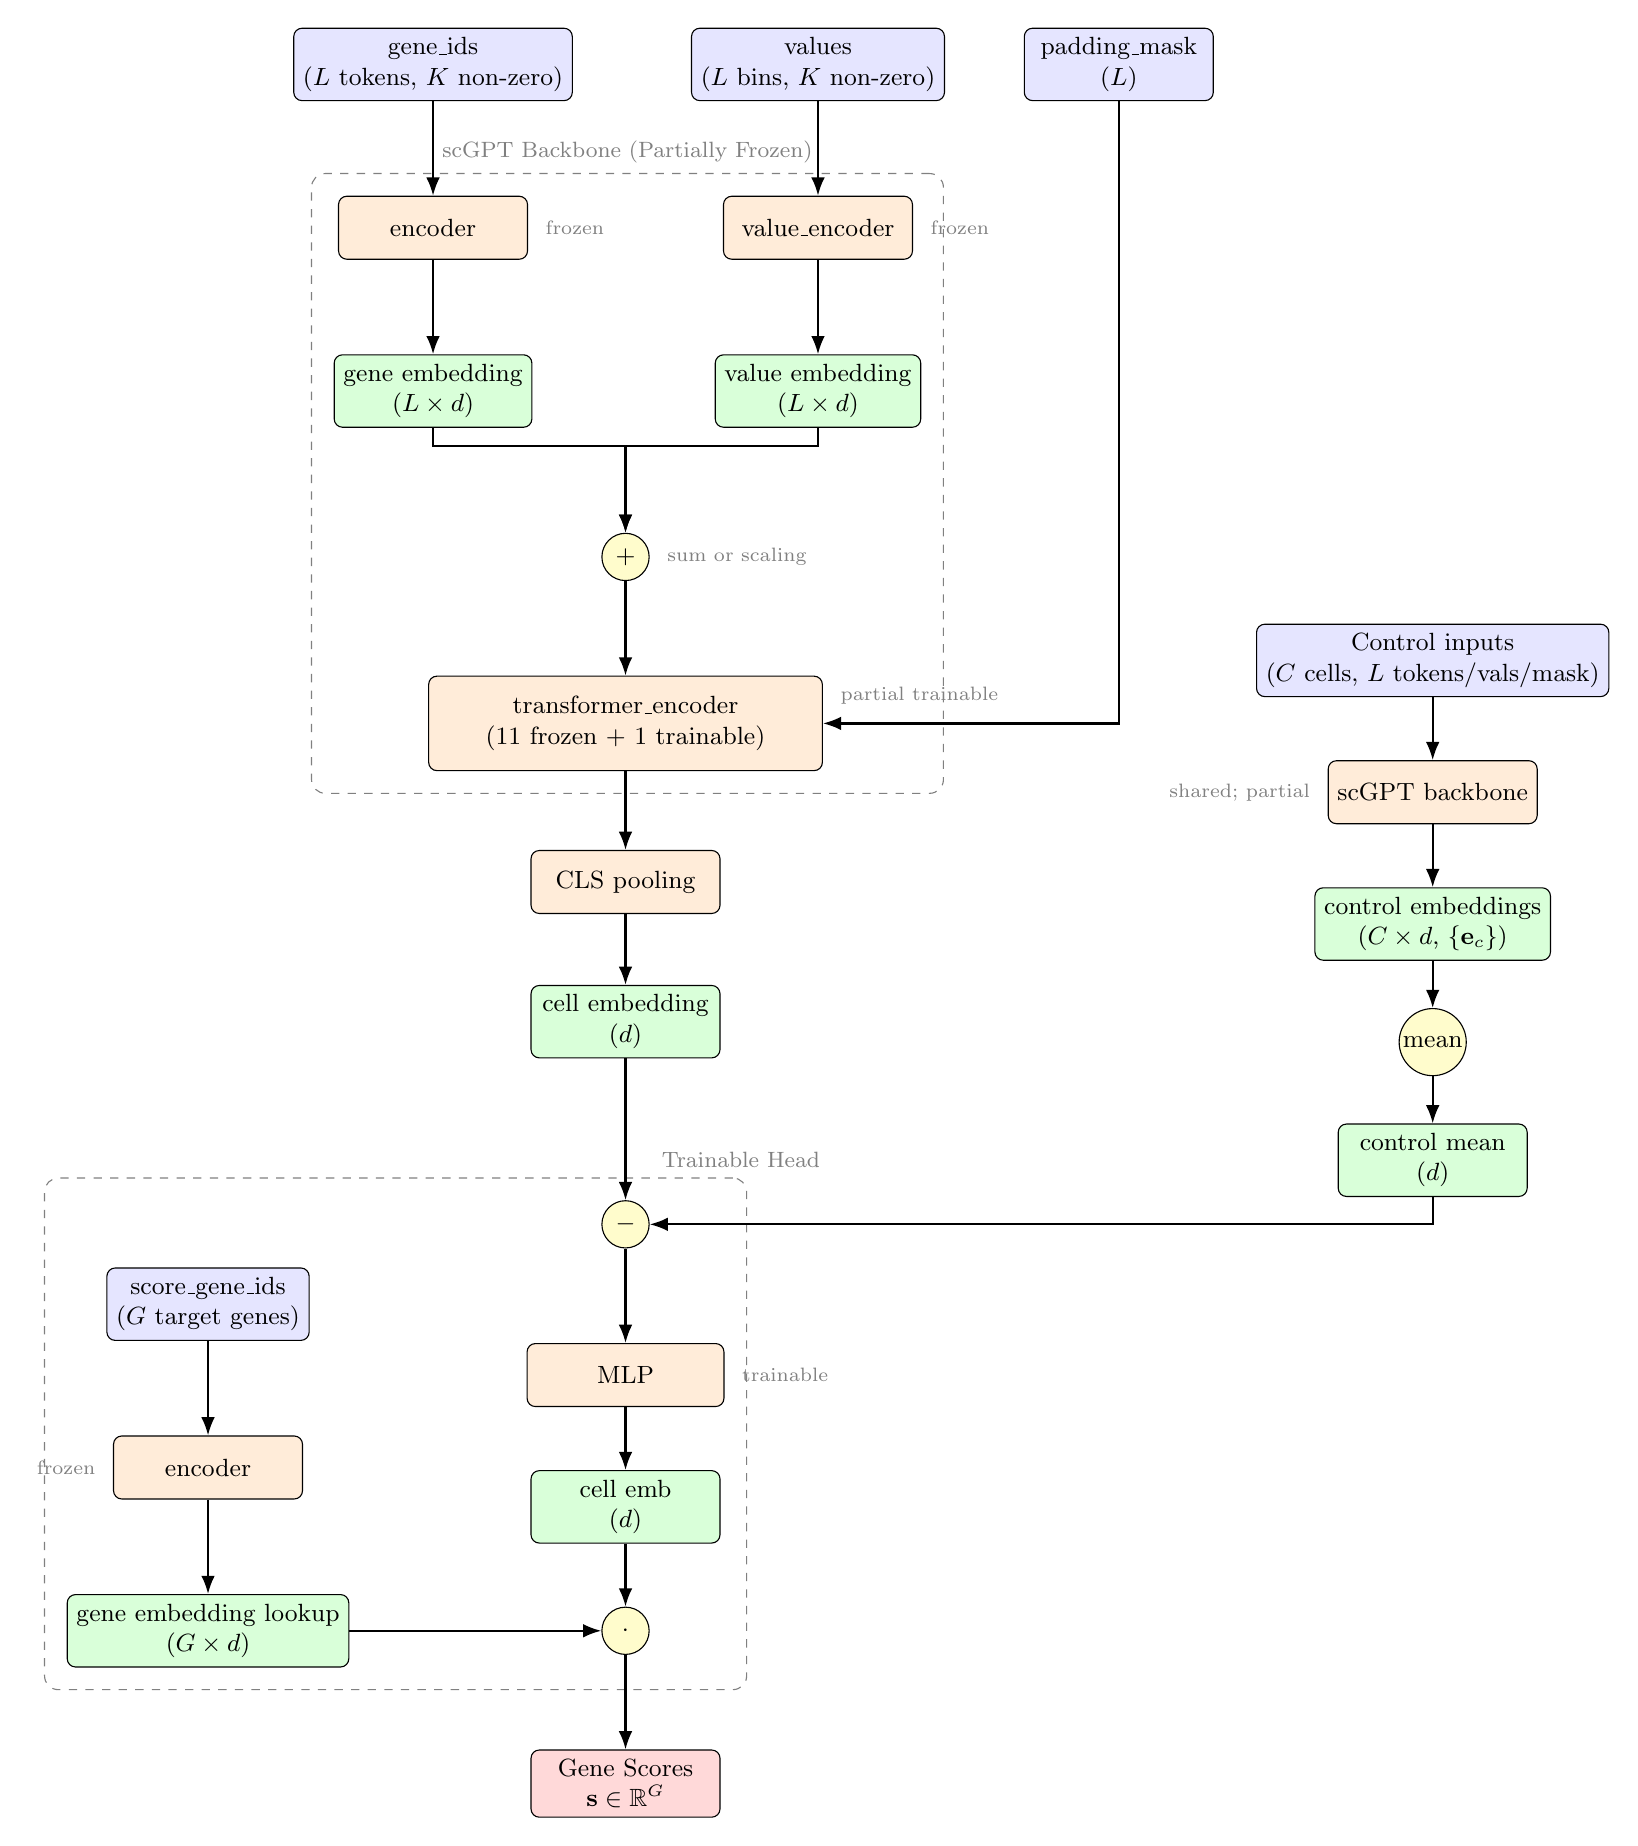
\begin{tikzpicture}[
    >=Latex,
    node distance=1.2cm and 2.4cm,
    font=\small,
    % Style definitions
    input/.style={draw, rounded corners=3pt, minimum width=2.4cm, minimum height=0.8cm, fill=blue!10, align=center},
    embed/.style={draw, rounded corners=3pt, minimum width=2.4cm, minimum height=0.8cm, fill=green!15, align=center},
    encoder/.style={draw, rounded corners=3pt, minimum width=2.4cm, minimum height=0.8cm, fill=orange!15, align=center},
    head/.style={draw, rounded corners=3pt, minimum width=2.4cm, minimum height=0.8cm, fill=yellow!15, align=center},
    unused/.style={draw, rounded corners=3pt, minimum width=2.4cm, minimum height=0.8cm, fill=gray!10, align=center, dashed},
    output/.style={draw, rounded corners=3pt, minimum width=2.4cm, minimum height=0.8cm, fill=red!15, align=center},
    operation/.style={circle, draw, minimum size=0.6cm, fill=yellow!20, inner sep=1pt},
    dashedbox/.style={draw, dashed, rounded corners=5pt, inner sep=8pt, gray},
    arrow/.style={->, thick, >=Latex, black},
]

%% ---------- INPUT LAYER ----------
\node[input] (gene_ids) {gene\_ids\\($L$ tokens, $K$ non-zero)};
\node[input, right=1.5cm of gene_ids] (values) {values\\($L$ bins, $K$ non-zero)};
\node[input, right=1cm of values] (padding) {padding\_mask\\($L$)};

%% ---------- ENCODERS + EMBEDDINGS (PARALLEL) ----------
\node[encoder, below=of gene_ids] (gene_encoder) {encoder};
\node[embed, below=of gene_encoder] (gene_emb) {gene embedding\\($L \times d$)};
\node[encoder, below=of values] (value_encoder) {value\_encoder};
\node[embed, below=of value_encoder] (value_emb) {value embedding\\($L \times d$)};

%% ---------- EMBEDDING FUSION ----------
\node[operation, below=1.8cm of $(gene_emb)!0.5!(value_emb)$] (add) {$+$};
\node[font=\scriptsize, gray, right=0.1cm of add.east] {sum or scaling};

%% ---------- TRANSFORMER ----------
\node[encoder, below=of add, minimum width=5cm, minimum height=1.2cm] (transformer) {transformer\_encoder\\(11 frozen + 1 trainable)};

%% ---------- OUTPUTS FROM TRANSFORMER ----------
\node[encoder, below=1.0cm of transformer] (cls_pool) {CLS pooling};
\node[embed, below=0.9cm of cls_pool] (cell_emb) {cell embedding\\($d$)};

%% ---------- CONTROL BRANCH ----------
\node[input, right=5.5cm of transformer, yshift=0.8cm] (control_branch) {Control inputs\\($C$ cells, $L$ tokens/vals/mask)};
\node[encoder, below=0.8cm of control_branch] (control_encoder) {scGPT backbone};
\node[embed, below=0.8cm of control_encoder] (control_emb) {control embeddings\\($C \times d$, $\{\mathbf{e}_c\}$)};
\node[operation, below=0.6cm of control_emb] (control_mean_op) {mean};
\node[embed, below=0.6cm of control_mean_op] (control_mean) {control mean\\($d$)};

%% ---------- DELTA EMBEDDING ----------
\node[operation, below=1.8cm of cell_emb] (subtract) {$-$};

%% ---------- GENE SCORING HEAD ----------
\node[encoder, below=of subtract, minimum width=2.5cm] (proj_mlp) {MLP};
\node[embed, below=0.8cm of proj_mlp] (cell_proj) {cell emb\\($d$)};
\node[operation, below=0.8cm of cell_proj] (dot_op) {$\cdot$};

%% ---------- OUTPUT ----------
\node[output, below=of dot_op] (scores) {Gene Scores\\$\mathbf{s} \in \mathbb{R}^{G}$};

%% ========== ARROWS ==========

% Inputs to encoders/embeddings
\draw[arrow] (gene_ids) -- (gene_encoder);
\draw[arrow] (gene_encoder) -- (gene_emb);
\draw[arrow] (values) -- (value_encoder);
\draw[arrow] (value_encoder) -- (value_emb);

% Embeddings to fusion (parallel)
\draw[arrow] (gene_emb) -- ++(0,-0.7) -| (add);
\draw[arrow] (value_emb) -- ++(0,-0.7) -| (add);

% Fusion to transformer
\draw[arrow] (add) -- (transformer);
\draw[arrow] (padding) |- (transformer);

% Transformer to cell embedding
\draw[arrow] (transformer.south) -- (cls_pool.north);
\draw[arrow] (cls_pool.south) -- (cell_emb.north);

% Control branch
\draw[arrow] (control_branch) -- (control_encoder);
\draw[arrow] (control_encoder) -- (control_emb);
\draw[arrow] (control_emb) -- (control_mean_op);
\draw[arrow] (control_mean_op) -- (control_mean);
\draw[arrow] (control_mean.south) |- (subtract.east);

% Cell embedding to delta
\draw[arrow] (cell_emb) -- (subtract);

% Delta to projection MLP
\draw[arrow] (subtract) -- (proj_mlp);
\draw[arrow] (proj_mlp) -- (cell_proj);
\draw[arrow] (cell_proj) -- (dot_op);

% Dot product to output
\draw[arrow] (dot_op) -- (scores);

% Gene embeddings to dot product (parallel flow)
\node[embed, left=3.2cm of dot_op] (gene_emb_lookup) {gene embedding lookup\\($G \times d$)};
\node[encoder, above=of gene_emb_lookup] (gene_emb_lookup_enc) {encoder};
\node[input, above=of gene_emb_lookup_enc] (score_gene_ids) {score\_gene\_ids\\($G$ target genes)};
\draw[arrow] (score_gene_ids) -- (gene_emb_lookup_enc);
\draw[arrow] (gene_emb_lookup_enc) -- (gene_emb_lookup);
\draw[arrow] (gene_emb_lookup.east) -- (dot_op.west);

%% ========== DASHED BOXES FOR GROUPING ==========

% scGPT Backbone box
\begin{scope}[on background layer]
    \node[dashedbox, fit=(gene_encoder)(value_encoder)(gene_emb)(value_emb)(add)(transformer), label={[font=\footnotesize, gray]above:scGPT Backbone (Partially Frozen)}] {};
\end{scope}

% Discriminative Head box
\begin{scope}[on background layer]
    \node[dashedbox, fit=(subtract)(proj_mlp)(cell_proj)(dot_op)(score_gene_ids)(gene_emb_lookup_enc)(gene_emb_lookup), label={[font=\footnotesize, gray]above right:Trainable Head}] {};
\end{scope}

%% ========== ANNOTATIONS ==========

% Trainability annotations
\node[font=\scriptsize, gray, right=0.1cm of gene_encoder.east] {frozen};
\node[font=\scriptsize, gray, right=0.1cm of value_encoder.east] {frozen};
\node[font=\scriptsize, gray, right=0.1cm of transformer.east, yshift=0.35cm] {partial trainable};
\node[font=\scriptsize, gray, left=0.1cm of control_encoder.west] {shared; partial};
\node[font=\scriptsize, gray, right=0.1cm of proj_mlp.east] {trainable};
\node[font=\scriptsize, gray, left=0.1cm of gene_emb_lookup_enc.west] {frozen};

\end{tikzpicture}
\ifexportfig
\else
\caption{Per-cell scGPT Discriminative Pipeline for Perturbation Gene Prediction.
For a single cell with $K$ non-zero genes, inputs are padded to length $L$.
Token IDs (\texttt{gene\_ids}), binned expression values, and a padding mask are fed to the scGPT backbone.
The \texttt{encoder} and \texttt{value\_encoder} produce gene/value embeddings, which are fused by element-wise addition (default)
or scaling (\texttt{input\_emb\_style}=\texttt{scaling}), then passed through \texttt{transformer\_encoder} to produce a CLS-based cell embedding.
A control branch runs the same backbone and the control mean is subtracted from the perturbed embedding.
The GeneScore head applies a projection MLP to the cell embedding before the dot product with the gene embedding lookup.
The \texttt{score\_gene\_ids} input is length $G$, the full set of candidate target genes, and its order defines the score output columns.
The backbone is partially frozen in this setup, with only the last transformer layer(s) and encoder norm optionally trainable.
Here, $G$ is the total number of genes in the dataset, $C$ is the number of control cells per perturbed cell, and $d$ is the embedding size.}
\label{fig:scgpt_pipeline}
\fi
\end{figure}

\end{document}
"
%   dvisvgm --libgs=/opt/homebrew/lib/libgs.dylib -o docs/report/final_report/scGPT_pipeline_standalone.svg docs/report/final_report/scGPT_pipeline_standalone_export.dvi
%   gs -sDEVICE=pngalpha -r300 -o docs/report/final_report/scGPT_pipeline_standalone.png docs/report/final_report/scGPT_pipeline_standalone_export.pdf

\documentclass{article}
\usepackage[margin=1cm]{geometry}
\usepackage{tikz}
\usepackage{amsmath,amssymb}
\usetikzlibrary{arrows.meta, positioning, shapes.geometric, calc, fit, backgrounds}
\newif\ifexportfig
\ifdefined\EXPORTFIG
\exportfigtrue
\else
\exportfigfalse
\fi

\begin{document}
\pagecolor{white}

\begin{figure}[htbp]
\centering
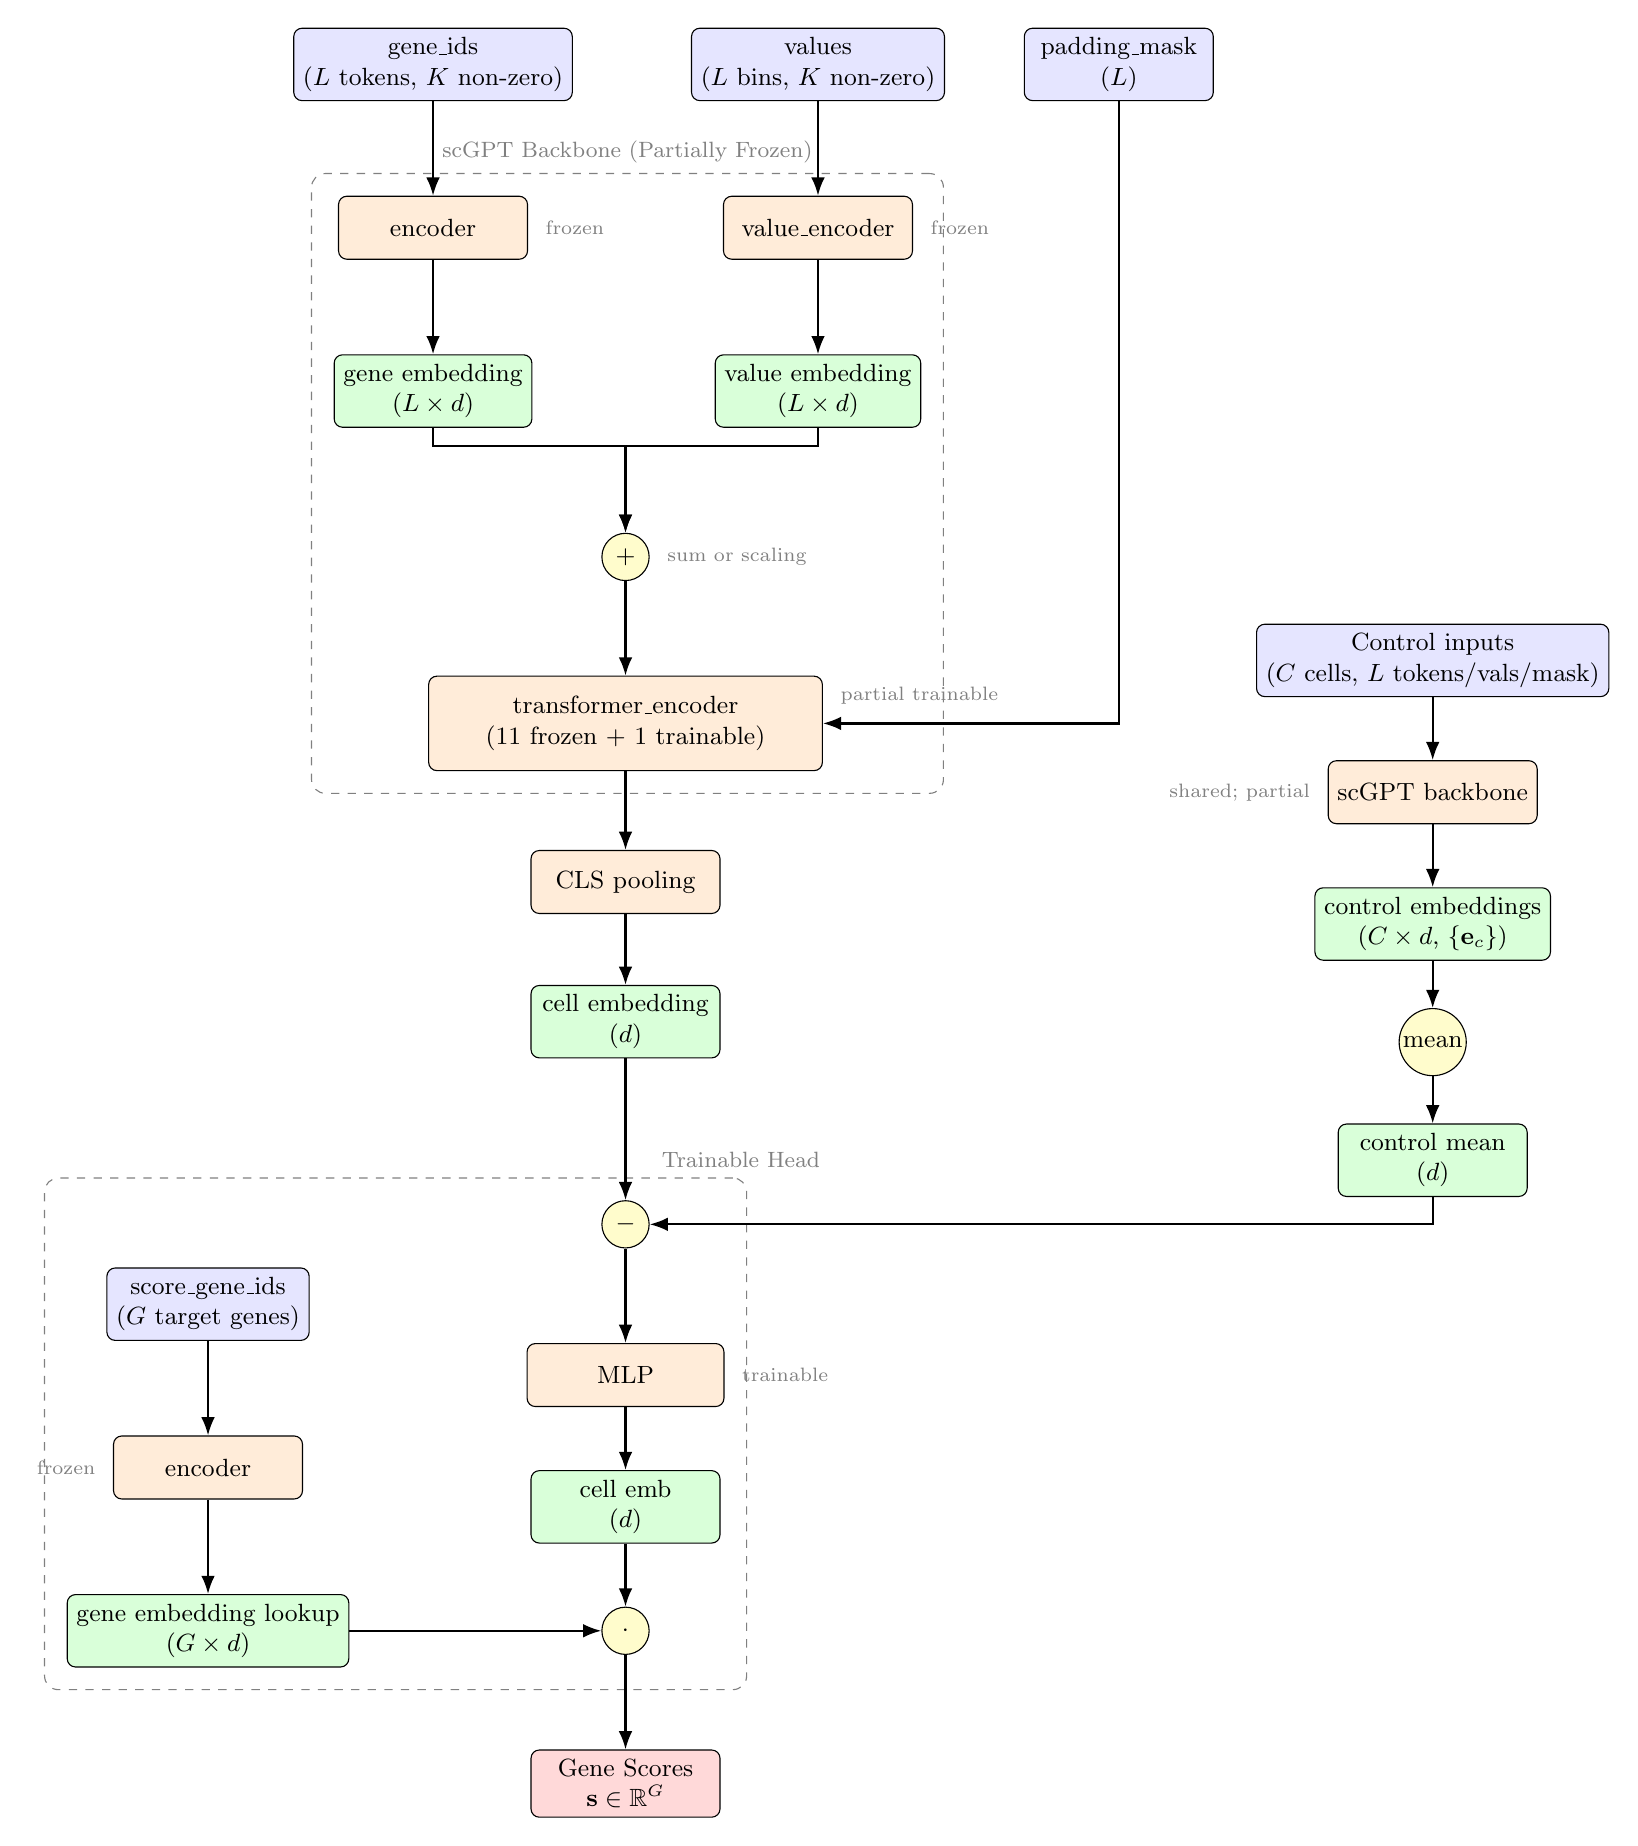
\begin{tikzpicture}[
    >=Latex,
    node distance=1.2cm and 2.4cm,
    font=\small,
    % Style definitions
    input/.style={draw, rounded corners=3pt, minimum width=2.4cm, minimum height=0.8cm, fill=blue!10, align=center},
    embed/.style={draw, rounded corners=3pt, minimum width=2.4cm, minimum height=0.8cm, fill=green!15, align=center},
    encoder/.style={draw, rounded corners=3pt, minimum width=2.4cm, minimum height=0.8cm, fill=orange!15, align=center},
    head/.style={draw, rounded corners=3pt, minimum width=2.4cm, minimum height=0.8cm, fill=yellow!15, align=center},
    unused/.style={draw, rounded corners=3pt, minimum width=2.4cm, minimum height=0.8cm, fill=gray!10, align=center, dashed},
    output/.style={draw, rounded corners=3pt, minimum width=2.4cm, minimum height=0.8cm, fill=red!15, align=center},
    operation/.style={circle, draw, minimum size=0.6cm, fill=yellow!20, inner sep=1pt},
    dashedbox/.style={draw, dashed, rounded corners=5pt, inner sep=8pt, gray},
    arrow/.style={->, thick, >=Latex, black},
]

%% ---------- INPUT LAYER ----------
\node[input] (gene_ids) {gene\_ids\\($L$ tokens, $K$ non-zero)};
\node[input, right=1.5cm of gene_ids] (values) {values\\($L$ bins, $K$ non-zero)};
\node[input, right=1cm of values] (padding) {padding\_mask\\($L$)};

%% ---------- ENCODERS + EMBEDDINGS (PARALLEL) ----------
\node[encoder, below=of gene_ids] (gene_encoder) {encoder};
\node[embed, below=of gene_encoder] (gene_emb) {gene embedding\\($L \times d$)};
\node[encoder, below=of values] (value_encoder) {value\_encoder};
\node[embed, below=of value_encoder] (value_emb) {value embedding\\($L \times d$)};

%% ---------- EMBEDDING FUSION ----------
\node[operation, below=1.8cm of $(gene_emb)!0.5!(value_emb)$] (add) {$+$};
\node[font=\scriptsize, gray, right=0.1cm of add.east] {sum or scaling};

%% ---------- TRANSFORMER ----------
\node[encoder, below=of add, minimum width=5cm, minimum height=1.2cm] (transformer) {transformer\_encoder\\(11 frozen + 1 trainable)};

%% ---------- OUTPUTS FROM TRANSFORMER ----------
\node[encoder, below=1.0cm of transformer] (cls_pool) {CLS pooling};
\node[embed, below=0.9cm of cls_pool] (cell_emb) {cell embedding\\($d$)};

%% ---------- CONTROL BRANCH ----------
\node[input, right=5.5cm of transformer, yshift=0.8cm] (control_branch) {Control inputs\\($C$ cells, $L$ tokens/vals/mask)};
\node[encoder, below=0.8cm of control_branch] (control_encoder) {scGPT backbone};
\node[embed, below=0.8cm of control_encoder] (control_emb) {control embeddings\\($C \times d$, $\{\mathbf{e}_c\}$)};
\node[operation, below=0.6cm of control_emb] (control_mean_op) {mean};
\node[embed, below=0.6cm of control_mean_op] (control_mean) {control mean\\($d$)};

%% ---------- DELTA EMBEDDING ----------
\node[operation, below=1.8cm of cell_emb] (subtract) {$-$};

%% ---------- GENE SCORING HEAD ----------
\node[encoder, below=of subtract, minimum width=2.5cm] (proj_mlp) {MLP};
\node[embed, below=0.8cm of proj_mlp] (cell_proj) {cell emb\\($d$)};
\node[operation, below=0.8cm of cell_proj] (dot_op) {$\cdot$};

%% ---------- OUTPUT ----------
\node[output, below=of dot_op] (scores) {Gene Scores\\$\mathbf{s} \in \mathbb{R}^{G}$};

%% ========== ARROWS ==========

% Inputs to encoders/embeddings
\draw[arrow] (gene_ids) -- (gene_encoder);
\draw[arrow] (gene_encoder) -- (gene_emb);
\draw[arrow] (values) -- (value_encoder);
\draw[arrow] (value_encoder) -- (value_emb);

% Embeddings to fusion (parallel)
\draw[arrow] (gene_emb) -- ++(0,-0.7) -| (add);
\draw[arrow] (value_emb) -- ++(0,-0.7) -| (add);

% Fusion to transformer
\draw[arrow] (add) -- (transformer);
\draw[arrow] (padding) |- (transformer);

% Transformer to cell embedding
\draw[arrow] (transformer.south) -- (cls_pool.north);
\draw[arrow] (cls_pool.south) -- (cell_emb.north);

% Control branch
\draw[arrow] (control_branch) -- (control_encoder);
\draw[arrow] (control_encoder) -- (control_emb);
\draw[arrow] (control_emb) -- (control_mean_op);
\draw[arrow] (control_mean_op) -- (control_mean);
\draw[arrow] (control_mean.south) |- (subtract.east);

% Cell embedding to delta
\draw[arrow] (cell_emb) -- (subtract);

% Delta to projection MLP
\draw[arrow] (subtract) -- (proj_mlp);
\draw[arrow] (proj_mlp) -- (cell_proj);
\draw[arrow] (cell_proj) -- (dot_op);

% Dot product to output
\draw[arrow] (dot_op) -- (scores);

% Gene embeddings to dot product (parallel flow)
\node[embed, left=3.2cm of dot_op] (gene_emb_lookup) {gene embedding lookup\\($G \times d$)};
\node[encoder, above=of gene_emb_lookup] (gene_emb_lookup_enc) {encoder};
\node[input, above=of gene_emb_lookup_enc] (score_gene_ids) {score\_gene\_ids\\($G$ target genes)};
\draw[arrow] (score_gene_ids) -- (gene_emb_lookup_enc);
\draw[arrow] (gene_emb_lookup_enc) -- (gene_emb_lookup);
\draw[arrow] (gene_emb_lookup.east) -- (dot_op.west);

%% ========== DASHED BOXES FOR GROUPING ==========

% scGPT Backbone box
\begin{scope}[on background layer]
    \node[dashedbox, fit=(gene_encoder)(value_encoder)(gene_emb)(value_emb)(add)(transformer), label={[font=\footnotesize, gray]above:scGPT Backbone (Partially Frozen)}] {};
\end{scope}

% Discriminative Head box
\begin{scope}[on background layer]
    \node[dashedbox, fit=(subtract)(proj_mlp)(cell_proj)(dot_op)(score_gene_ids)(gene_emb_lookup_enc)(gene_emb_lookup), label={[font=\footnotesize, gray]above right:Trainable Head}] {};
\end{scope}

%% ========== ANNOTATIONS ==========

% Trainability annotations
\node[font=\scriptsize, gray, right=0.1cm of gene_encoder.east] {frozen};
\node[font=\scriptsize, gray, right=0.1cm of value_encoder.east] {frozen};
\node[font=\scriptsize, gray, right=0.1cm of transformer.east, yshift=0.35cm] {partial trainable};
\node[font=\scriptsize, gray, left=0.1cm of control_encoder.west] {shared; partial};
\node[font=\scriptsize, gray, right=0.1cm of proj_mlp.east] {trainable};
\node[font=\scriptsize, gray, left=0.1cm of gene_emb_lookup_enc.west] {frozen};

\end{tikzpicture}
\ifexportfig
\else
\caption{Per-cell scGPT Discriminative Pipeline for Perturbation Gene Prediction.
For a single cell with $K$ non-zero genes, inputs are padded to length $L$.
Token IDs (\texttt{gene\_ids}), binned expression values, and a padding mask are fed to the scGPT backbone.
The \texttt{encoder} and \texttt{value\_encoder} produce gene/value embeddings, which are fused by element-wise addition (default)
or scaling (\texttt{input\_emb\_style}=\texttt{scaling}), then passed through \texttt{transformer\_encoder} to produce a CLS-based cell embedding.
A control branch runs the same backbone and the control mean is subtracted from the perturbed embedding.
The GeneScore head applies a projection MLP to the cell embedding before the dot product with the gene embedding lookup.
The \texttt{score\_gene\_ids} input is length $G$, the full set of candidate target genes, and its order defines the score output columns.
The backbone is partially frozen in this setup, with only the last transformer layer(s) and encoder norm optionally trainable.
Here, $G$ is the total number of genes in the dataset, $C$ is the number of control cells per perturbed cell, and $d$ is the embedding size.}
\label{fig:scgpt_pipeline}
\fi
\end{figure}

\end{document}
"
%   dvisvgm --libgs=/opt/homebrew/lib/libgs.dylib -o docs/report/final_report/scGPT_pipeline_standalone.svg docs/report/final_report/scGPT_pipeline_standalone_export.dvi
%   gs -sDEVICE=pngalpha -r300 -o docs/report/final_report/scGPT_pipeline_standalone.png docs/report/final_report/scGPT_pipeline_standalone_export.pdf

\documentclass{article}
\usepackage[margin=1cm]{geometry}
\usepackage{tikz}
\usepackage{amsmath,amssymb}
\usetikzlibrary{arrows.meta, positioning, shapes.geometric, calc, fit, backgrounds}
\newif\ifexportfig
\ifdefined\EXPORTFIG
\exportfigtrue
\else
\exportfigfalse
\fi

\begin{document}
\pagecolor{white}

\begin{figure}[htbp]
\centering
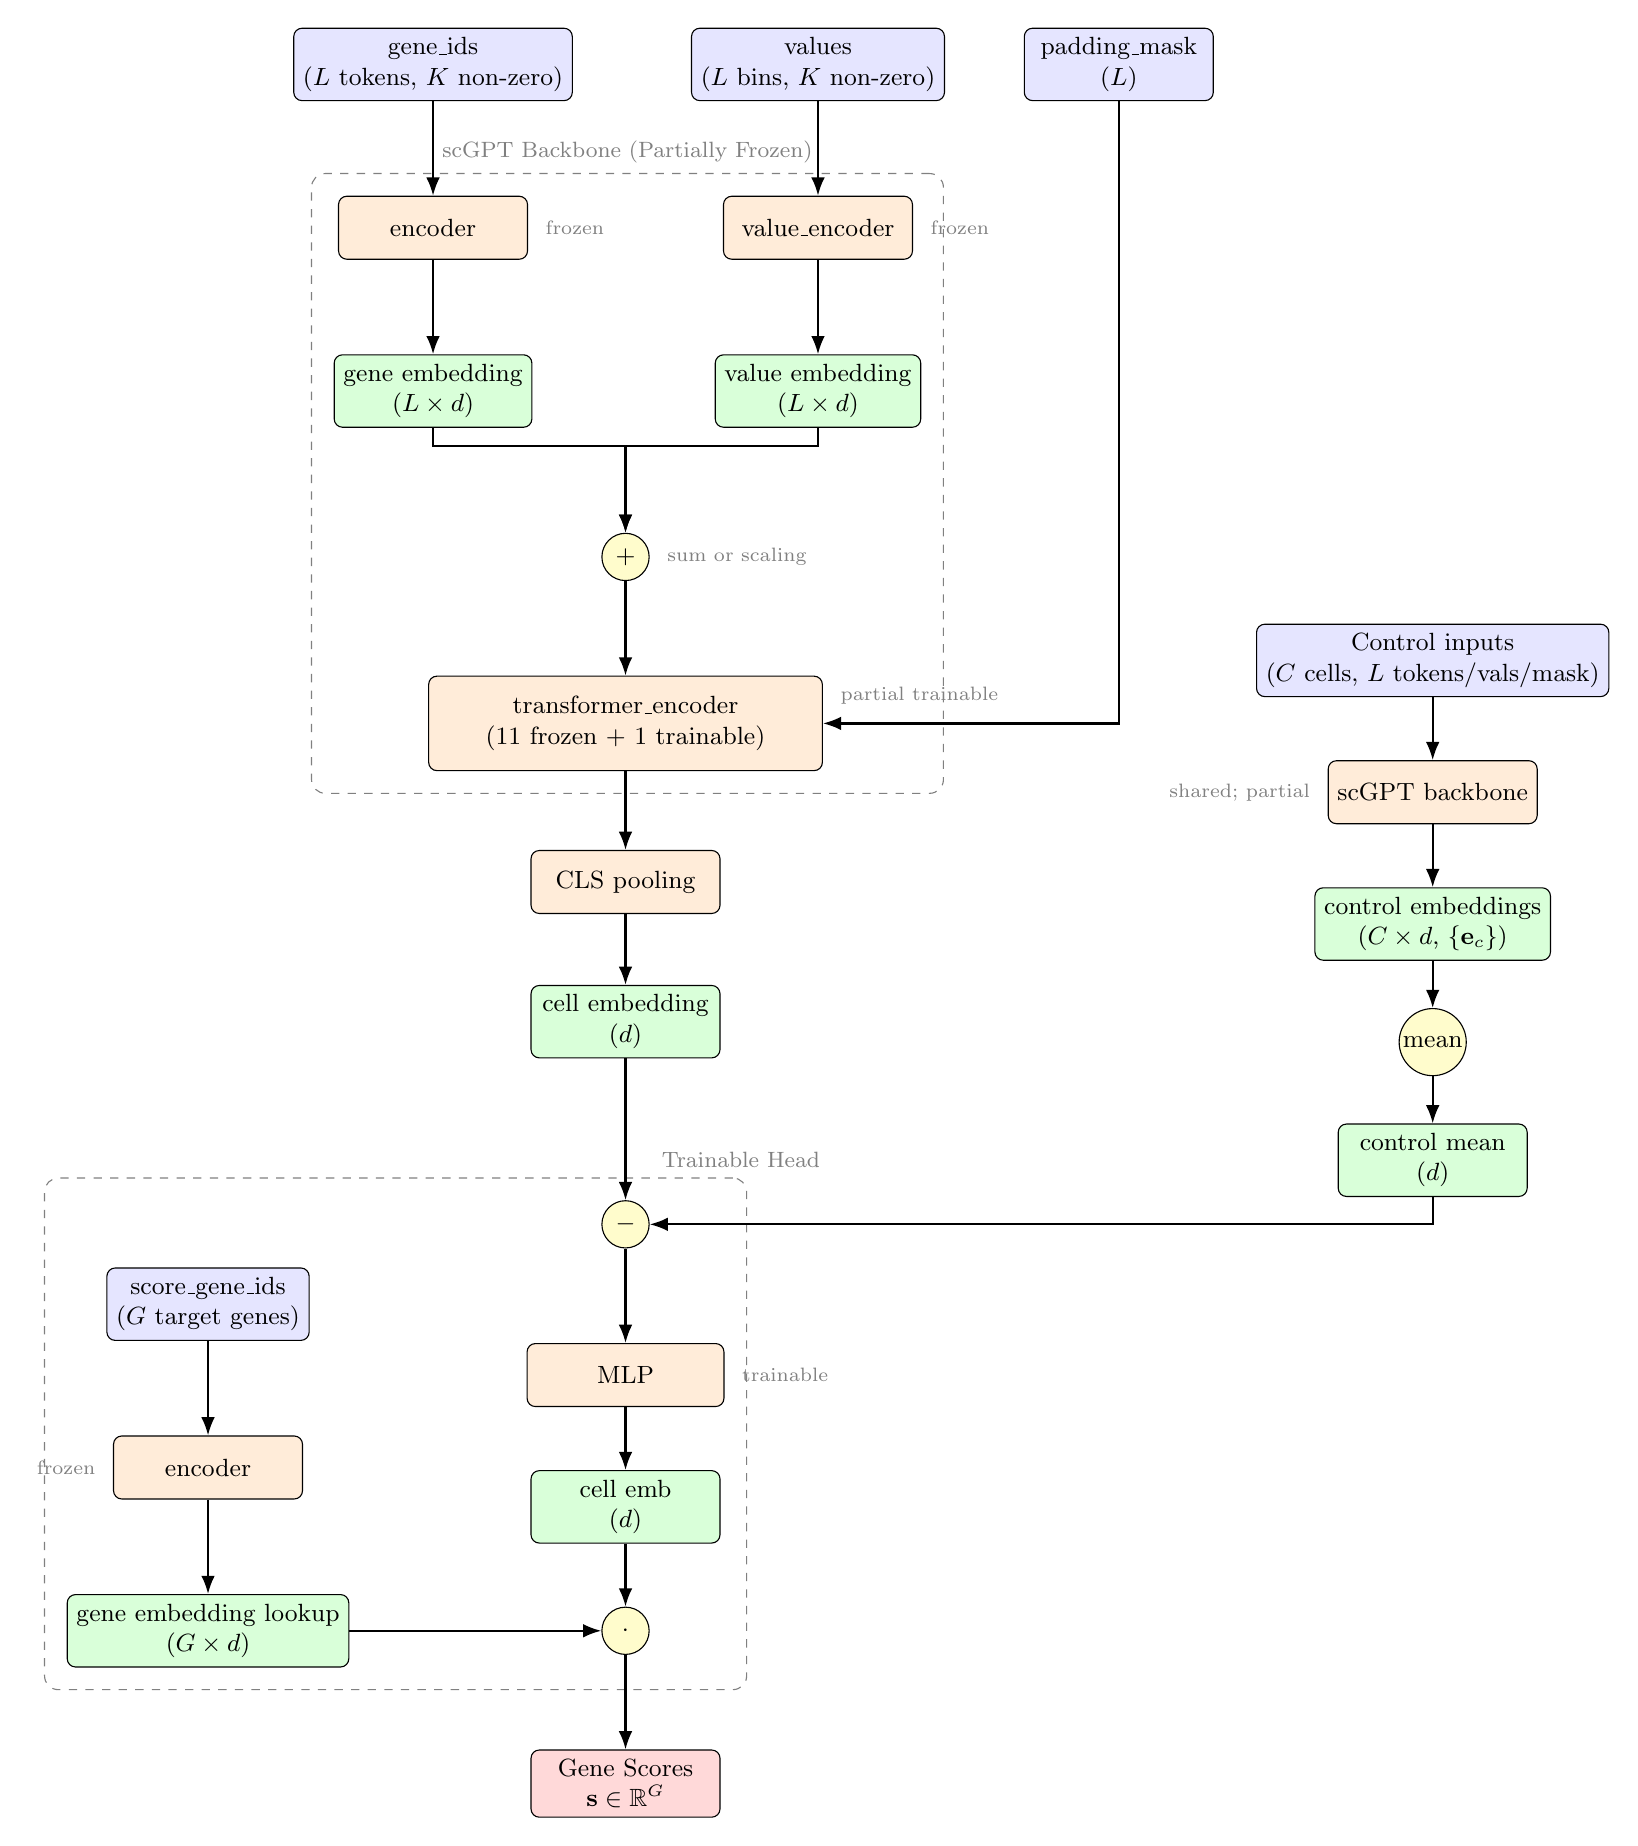
\begin{tikzpicture}[
    >=Latex,
    node distance=1.2cm and 2.4cm,
    font=\small,
    % Style definitions
    input/.style={draw, rounded corners=3pt, minimum width=2.4cm, minimum height=0.8cm, fill=blue!10, align=center},
    embed/.style={draw, rounded corners=3pt, minimum width=2.4cm, minimum height=0.8cm, fill=green!15, align=center},
    encoder/.style={draw, rounded corners=3pt, minimum width=2.4cm, minimum height=0.8cm, fill=orange!15, align=center},
    head/.style={draw, rounded corners=3pt, minimum width=2.4cm, minimum height=0.8cm, fill=yellow!15, align=center},
    unused/.style={draw, rounded corners=3pt, minimum width=2.4cm, minimum height=0.8cm, fill=gray!10, align=center, dashed},
    output/.style={draw, rounded corners=3pt, minimum width=2.4cm, minimum height=0.8cm, fill=red!15, align=center},
    operation/.style={circle, draw, minimum size=0.6cm, fill=yellow!20, inner sep=1pt},
    dashedbox/.style={draw, dashed, rounded corners=5pt, inner sep=8pt, gray},
    arrow/.style={->, thick, >=Latex, black},
]

%% ---------- INPUT LAYER ----------
\node[input] (gene_ids) {gene\_ids\\($L$ tokens, $K$ non-zero)};
\node[input, right=1.5cm of gene_ids] (values) {values\\($L$ bins, $K$ non-zero)};
\node[input, right=1cm of values] (padding) {padding\_mask\\($L$)};

%% ---------- ENCODERS + EMBEDDINGS (PARALLEL) ----------
\node[encoder, below=of gene_ids] (gene_encoder) {encoder};
\node[embed, below=of gene_encoder] (gene_emb) {gene embedding\\($L \times d$)};
\node[encoder, below=of values] (value_encoder) {value\_encoder};
\node[embed, below=of value_encoder] (value_emb) {value embedding\\($L \times d$)};

%% ---------- EMBEDDING FUSION ----------
\node[operation, below=1.8cm of $(gene_emb)!0.5!(value_emb)$] (add) {$+$};
\node[font=\scriptsize, gray, right=0.1cm of add.east] {sum or scaling};

%% ---------- TRANSFORMER ----------
\node[encoder, below=of add, minimum width=5cm, minimum height=1.2cm] (transformer) {transformer\_encoder\\(11 frozen + 1 trainable)};

%% ---------- OUTPUTS FROM TRANSFORMER ----------
\node[encoder, below=1.0cm of transformer] (cls_pool) {CLS pooling};
\node[embed, below=0.9cm of cls_pool] (cell_emb) {cell embedding\\($d$)};

%% ---------- CONTROL BRANCH ----------
\node[input, right=5.5cm of transformer, yshift=0.8cm] (control_branch) {Control inputs\\($C$ cells, $L$ tokens/vals/mask)};
\node[encoder, below=0.8cm of control_branch] (control_encoder) {scGPT backbone};
\node[embed, below=0.8cm of control_encoder] (control_emb) {control embeddings\\($C \times d$, $\{\mathbf{e}_c\}$)};
\node[operation, below=0.6cm of control_emb] (control_mean_op) {mean};
\node[embed, below=0.6cm of control_mean_op] (control_mean) {control mean\\($d$)};

%% ---------- DELTA EMBEDDING ----------
\node[operation, below=1.8cm of cell_emb] (subtract) {$-$};

%% ---------- GENE SCORING HEAD ----------
\node[encoder, below=of subtract, minimum width=2.5cm] (proj_mlp) {MLP};
\node[embed, below=0.8cm of proj_mlp] (cell_proj) {cell emb\\($d$)};
\node[operation, below=0.8cm of cell_proj] (dot_op) {$\cdot$};

%% ---------- OUTPUT ----------
\node[output, below=of dot_op] (scores) {Gene Scores\\$\mathbf{s} \in \mathbb{R}^{G}$};

%% ========== ARROWS ==========

% Inputs to encoders/embeddings
\draw[arrow] (gene_ids) -- (gene_encoder);
\draw[arrow] (gene_encoder) -- (gene_emb);
\draw[arrow] (values) -- (value_encoder);
\draw[arrow] (value_encoder) -- (value_emb);

% Embeddings to fusion (parallel)
\draw[arrow] (gene_emb) -- ++(0,-0.7) -| (add);
\draw[arrow] (value_emb) -- ++(0,-0.7) -| (add);

% Fusion to transformer
\draw[arrow] (add) -- (transformer);
\draw[arrow] (padding) |- (transformer);

% Transformer to cell embedding
\draw[arrow] (transformer.south) -- (cls_pool.north);
\draw[arrow] (cls_pool.south) -- (cell_emb.north);

% Control branch
\draw[arrow] (control_branch) -- (control_encoder);
\draw[arrow] (control_encoder) -- (control_emb);
\draw[arrow] (control_emb) -- (control_mean_op);
\draw[arrow] (control_mean_op) -- (control_mean);
\draw[arrow] (control_mean.south) |- (subtract.east);

% Cell embedding to delta
\draw[arrow] (cell_emb) -- (subtract);

% Delta to projection MLP
\draw[arrow] (subtract) -- (proj_mlp);
\draw[arrow] (proj_mlp) -- (cell_proj);
\draw[arrow] (cell_proj) -- (dot_op);

% Dot product to output
\draw[arrow] (dot_op) -- (scores);

% Gene embeddings to dot product (parallel flow)
\node[embed, left=3.2cm of dot_op] (gene_emb_lookup) {gene embedding lookup\\($G \times d$)};
\node[encoder, above=of gene_emb_lookup] (gene_emb_lookup_enc) {encoder};
\node[input, above=of gene_emb_lookup_enc] (score_gene_ids) {score\_gene\_ids\\($G$ target genes)};
\draw[arrow] (score_gene_ids) -- (gene_emb_lookup_enc);
\draw[arrow] (gene_emb_lookup_enc) -- (gene_emb_lookup);
\draw[arrow] (gene_emb_lookup.east) -- (dot_op.west);

%% ========== DASHED BOXES FOR GROUPING ==========

% scGPT Backbone box
\begin{scope}[on background layer]
    \node[dashedbox, fit=(gene_encoder)(value_encoder)(gene_emb)(value_emb)(add)(transformer), label={[font=\footnotesize, gray]above:scGPT Backbone (Partially Frozen)}] {};
\end{scope}

% Discriminative Head box
\begin{scope}[on background layer]
    \node[dashedbox, fit=(subtract)(proj_mlp)(cell_proj)(dot_op)(score_gene_ids)(gene_emb_lookup_enc)(gene_emb_lookup), label={[font=\footnotesize, gray]above right:Trainable Head}] {};
\end{scope}

%% ========== ANNOTATIONS ==========

% Trainability annotations
\node[font=\scriptsize, gray, right=0.1cm of gene_encoder.east] {frozen};
\node[font=\scriptsize, gray, right=0.1cm of value_encoder.east] {frozen};
\node[font=\scriptsize, gray, right=0.1cm of transformer.east, yshift=0.35cm] {partial trainable};
\node[font=\scriptsize, gray, left=0.1cm of control_encoder.west] {shared; partial};
\node[font=\scriptsize, gray, right=0.1cm of proj_mlp.east] {trainable};
\node[font=\scriptsize, gray, left=0.1cm of gene_emb_lookup_enc.west] {frozen};

\end{tikzpicture}
\ifexportfig
\else
\caption{Per-cell scGPT Discriminative Pipeline for Perturbation Gene Prediction.
For a single cell with $K$ non-zero genes, inputs are padded to length $L$.
Token IDs (\texttt{gene\_ids}), binned expression values, and a padding mask are fed to the scGPT backbone.
The \texttt{encoder} and \texttt{value\_encoder} produce gene/value embeddings, which are fused by element-wise addition (default)
or scaling (\texttt{input\_emb\_style}=\texttt{scaling}), then passed through \texttt{transformer\_encoder} to produce a CLS-based cell embedding.
A control branch runs the same backbone and the control mean is subtracted from the perturbed embedding.
The GeneScore head applies a projection MLP to the cell embedding before the dot product with the gene embedding lookup.
The \texttt{score\_gene\_ids} input is length $G$, the full set of candidate target genes, and its order defines the score output columns.
The backbone is partially frozen in this setup, with only the last transformer layer(s) and encoder norm optionally trainable.
Here, $G$ is the total number of genes in the dataset, $C$ is the number of control cells per perturbed cell, and $d$ is the embedding size.}
\label{fig:scgpt_pipeline}
\fi
\end{figure}

\end{document}
